This section contains the list of the S\+DD.

\tabulinesep=1mm
\begin{longtabu} spread 0pt [c]{*2{|X[-1]}|}
\hline
\rowcolor{\tableheadbgcolor}{\bf Service }&{\bf Description  }\\\cline{1-2}
\endfirsthead
\hline
\endfoot
\hline
\rowcolor{\tableheadbgcolor}{\bf Service }&{\bf Description  }\\\cline{1-2}
\endhead
\hyperlink{c_SDD_audio}{Audio S\+DD} &audio design document \\\cline{1-2}
c\+\_\+\+S\+D\+D\+\_\+fwupdate\+\_\+\+Dual\+Sys &FW update on dual system platform document \\\cline{1-2}
\hyperlink{c_SDD_atClient}{AT client S\+DD} &AT client design document \\\cline{1-2}
\hyperlink{c_SDD_mdc}{Modem Data Control S\+DD} &Modem data control design document \\\cline{1-2}
\hyperlink{c_SDD_eCall}{e\+Call S\+DD} &e\+Call design document \\\cline{1-2}
\end{longtabu}
Copyright (C) Sierra Wireless Inc. \hypertarget{c_SDD_audio}{}\section{Audio S\+DD}\label{c_SDD_audio}
\hypertarget{c_SDD_audio_Multimedia}{}\subsection{Multimedia}\label{c_SDD_audio_Multimedia}
\hypertarget{c_SDD_mdc_Overview}{}\subsubsection{Overview}\label{c_SDD_mdc_Overview}
The Audio A\+PI handles audio interfaces including play and record supported formats. Four functionalities are proposed through the A\+P\+Is\+:
\begin{DoxyItemize}
\item file playback using \hyperlink{le__audio__interface_8h_aea2c5d0b394cfab87503639c534300c9}{le\+\_\+audio\+\_\+\+Play\+File()} A\+PI
\item file recording using \hyperlink{le__audio__interface_8h_a393a26f6cff7fe05c1813fcafeef50f3}{le\+\_\+audio\+\_\+\+Record\+File()} A\+PI
\item P\+CM samples playback using \hyperlink{le__audio__interface_8h_afd37d59ab8207338da197554f49d7ff0}{le\+\_\+audio\+\_\+\+Play\+Samples()} A\+PI
\item P\+CM samples recording using \hyperlink{le__audio__interface_8h_a9c55a59849afcbb2ccef88cd4265782e}{le\+\_\+audio\+\_\+\+Get\+Samples()} A\+PI
\end{DoxyItemize}

To provide these functionalities, audio daemon relies on a H\+AL (Harware Abstraction Layer) calling Alsa-\/intf to communicate with the sound driver A\+L\+SA. The audio platform adaptor uses the Alsa-\/intf\textquotesingle{}s open, read and write A\+P\+Is.~\newline
 For reading operation, Alsa-\/intf is configured in M\+M\+AP mode\+: Alsa-\/intf allocates a mmap buffer and provides it to the audio platform adaptor to get P\+CM frames to be played by A\+L\+SA.~\newline
 For write operation, Alsa-\/intf is configured in N\+M\+M\+AP mode\+: audio platform adaptor provides its own buffer to the Alsa-\/intf.

In play samples and get samples use cases, a pipe is created by the application to send/get audio samples to/from the audio daemon\textquotesingle{}threads in charge of the playback and the capture. To be generic, the same mechanism is re-\/used internally in the audio daemon for files playback and recording\+: a thread is in charge of sending and recording audio samples to the playback/capture threads through a pipe.

Playbacks A\+P\+Is are using the same Playback\+Thread thread\+: its goal is to read audio samples from a pipe, and send them to Alsa-\/intf to be played on sound device. Recording A\+P\+Is are using the same Capture\+Thread thread\+: its goal is to get audio samples from Alsa-\/intf, and write them into a pipe. These two threads are implemented in the audio platform adaptor. They are running until a stop operation is performed (by the application using the dedicated A\+PI \hyperlink{le__audio__interface_8h_a4aebc6e8cdc4389c375e93418823af71}{le\+\_\+audio\+\_\+\+Stop()}, or by the audio component when the end of the audio file is reached).

On the other end of the pipe, file playback and recording are using the media thread. Its goal is to\+:
\begin{DoxyItemize}
\item read samples and write into the pipe (playback file case). Read samples can be\+:
\begin{DoxyItemize}
\item read samples directly from a file (W\+AV files)
\item get samples from the A\+MR decoder (A\+M\+R-\/\+N\+B/\+A\+M\+R-\/\+WB files)
\item read samples from D\+T\+MF generator
\end{DoxyItemize}
\item read from the pipe and write into a file (capture case). Write samples can be\+:
\begin{DoxyItemize}
\item write samples directly into a file (W\+AV file)
\item record samples in A\+MR format (A\+M\+R-\/\+N\+B/\+A\+M\+R-\/\+WB files)
\end{DoxyItemize}
\end{DoxyItemize}\hypertarget{c_SDD_audio_le_audio_PlayFile}{}\subsubsection{le\+\_\+audio\+\_\+\+Play\+File}\label{c_SDD_audio_le_audio_PlayFile}
In play file use case, audio daemon starts the media and playback threads and creates a pipe to transfer P\+CM samples between both threads. Media thread is in charge of reading/decoding P\+CM frames and sending them on the pipe. Playback thread reads the P\+CM frames on the pipe and sends them to the sound driver through Alsa-\/intf.


\begin{DoxyImageNoCaption}
  \mbox{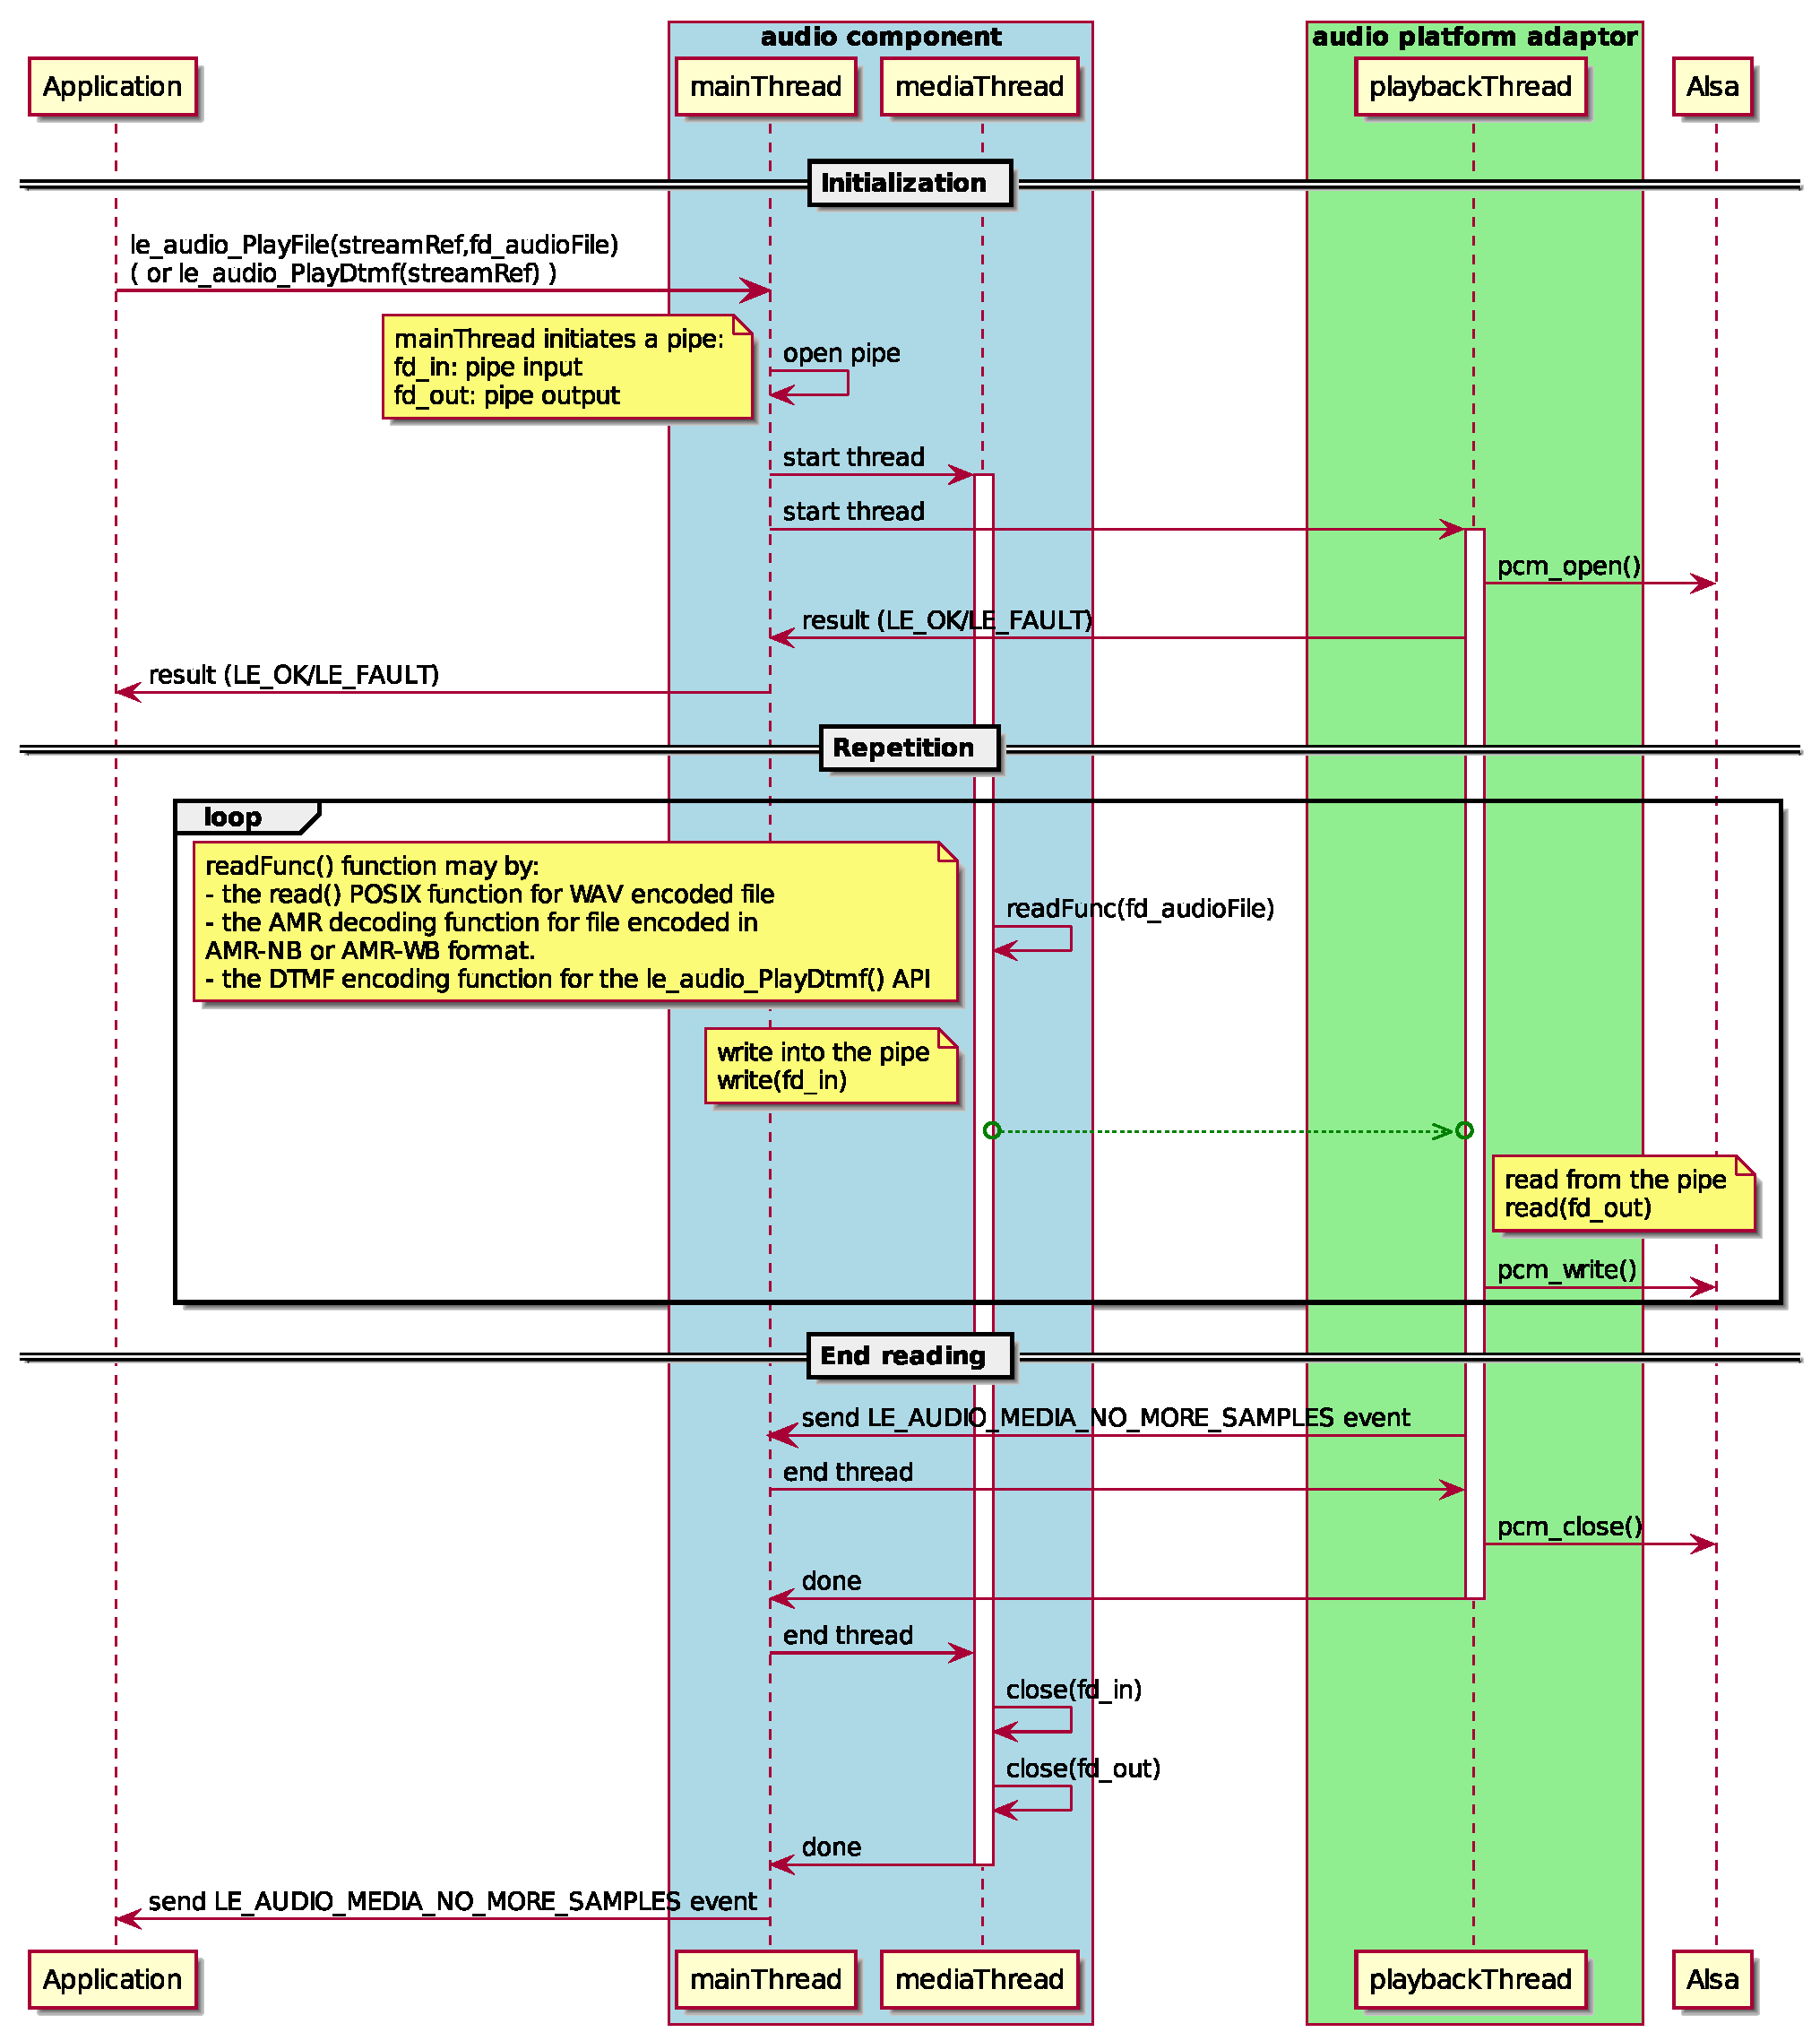
\includegraphics[width=\textwidth,height=\textheight/2,keepaspectratio=true]{le_audio_PlayFile}}
\end{DoxyImageNoCaption}
\hypertarget{c_SDD_audio_le_audio_PlaySamples}{}\subsubsection{le\+\_\+audio\+\_\+\+Play\+Samples}\label{c_SDD_audio_le_audio_PlaySamples}
In play samples use case, the application creates a pipe and sends P\+CM samples on it. In audio daemon side, playback thread is started to get the P\+CM samples from the pipe and then send them to the sound driver through Alsa-\/intf.


\begin{DoxyImageNoCaption}
  \mbox{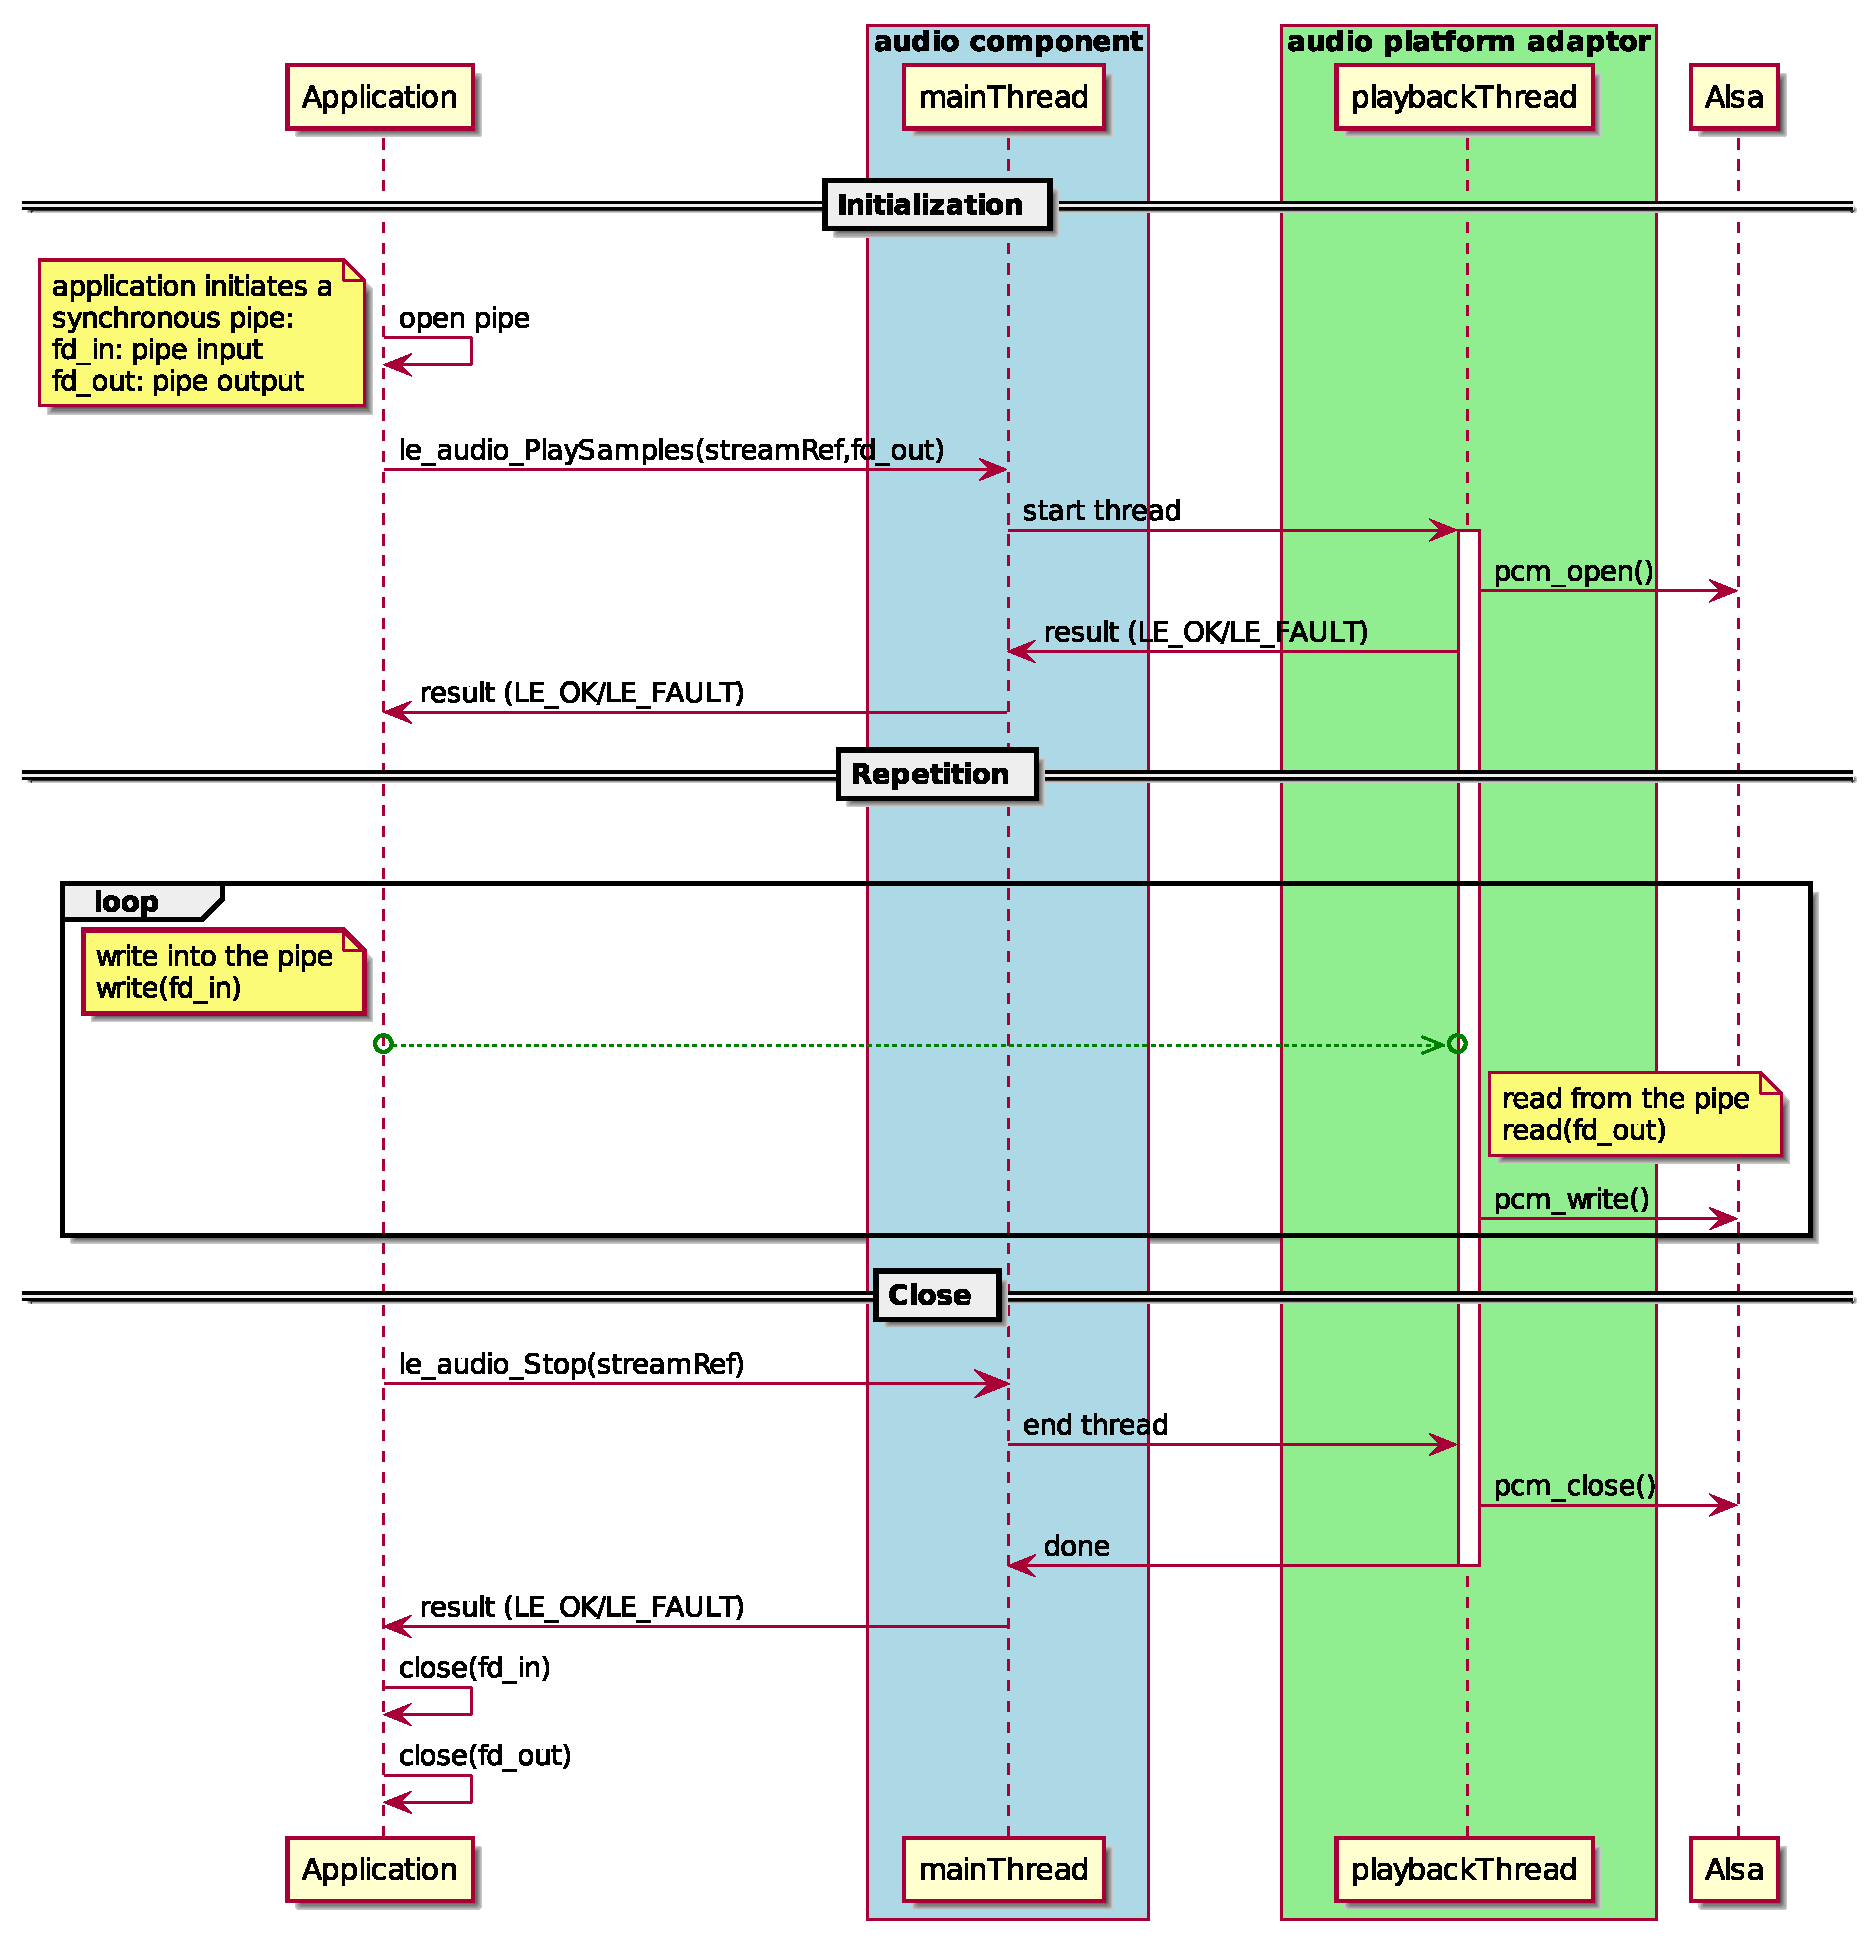
\includegraphics[width=\textwidth,height=\textheight/2,keepaspectratio=true]{le_audio_PlaySamples}}
\end{DoxyImageNoCaption}
\hypertarget{c_SDD_audio_le_audio_GetSamples}{}\subsubsection{le\+\_\+audio\+\_\+\+Get\+Samples}\label{c_SDD_audio_le_audio_GetSamples}
In get samples use case, the application creates a pipe and gets P\+CM samples on it. In audio daemon side, capture thread is started to get the P\+CM samples from Alsa-\/intf and then send them on the pipe to the application.


\begin{DoxyImageNoCaption}
  \mbox{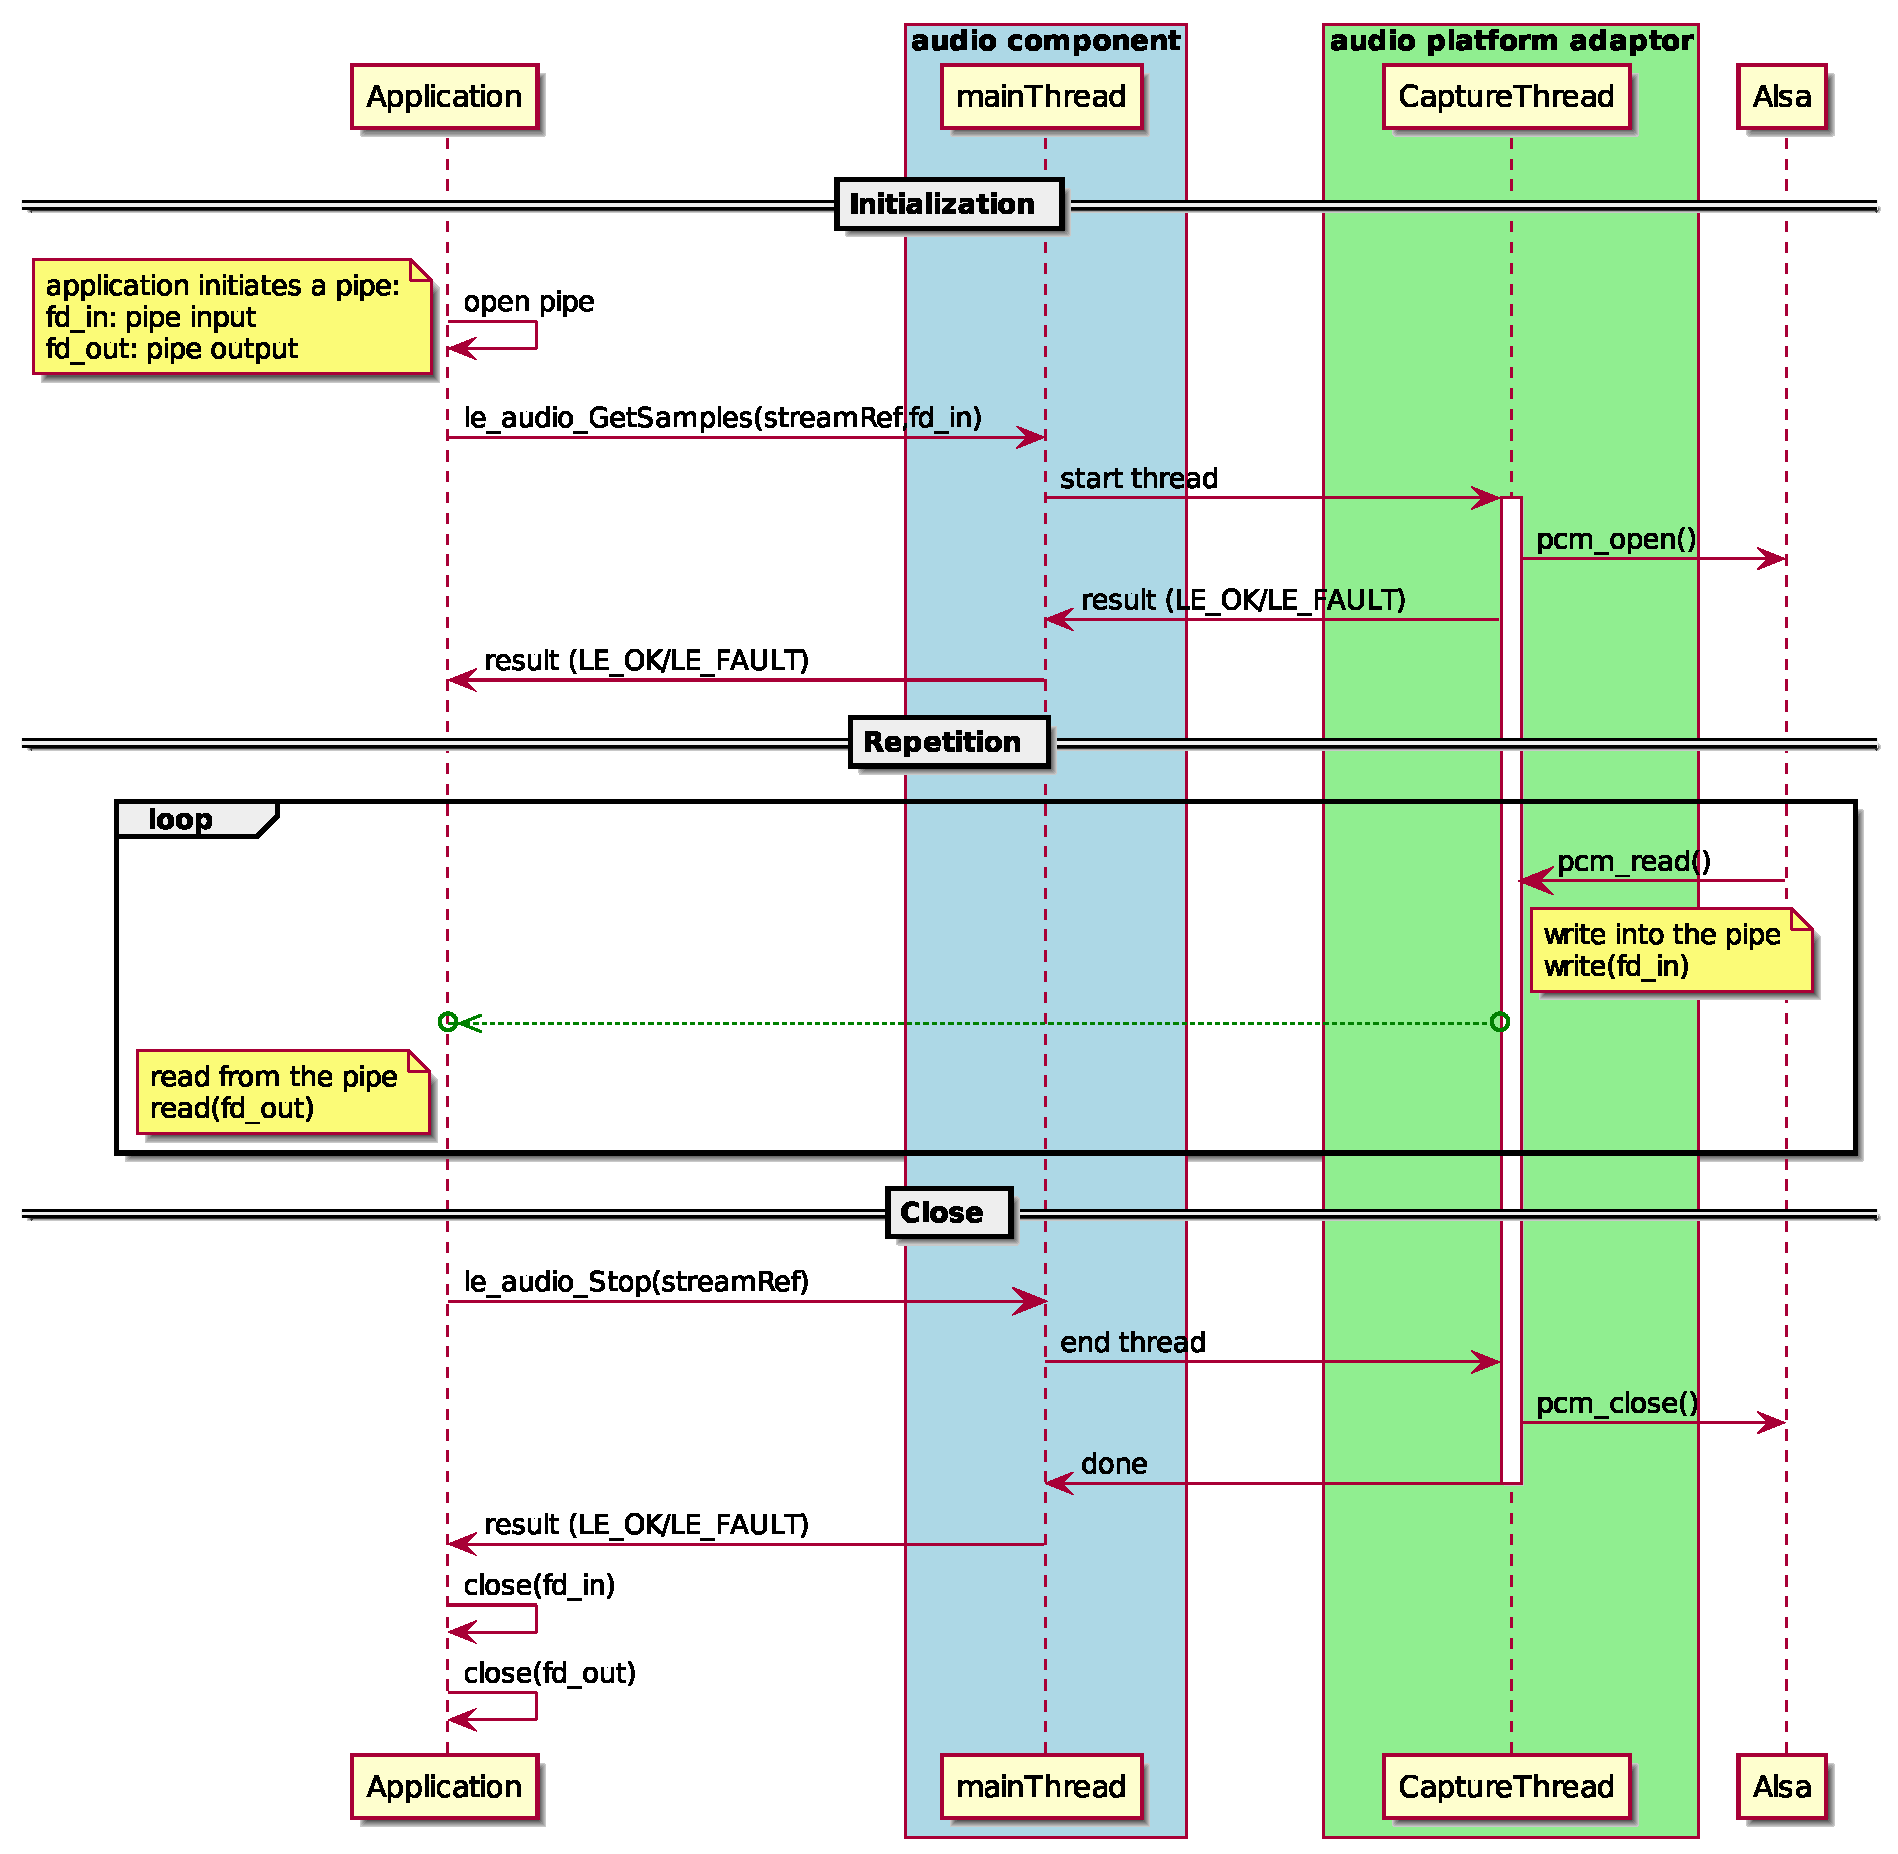
\includegraphics[width=\textwidth,height=\textheight/2,keepaspectratio=true]{le_audio_GetSamples}}
\end{DoxyImageNoCaption}
\hypertarget{c_SDD_audio_le_audio_RecordFile}{}\subsubsection{le\+\_\+audio\+\_\+\+Record\+File}\label{c_SDD_audio_le_audio_RecordFile}
In record file use case, audio daemon starts the media and capture threads, and creates a pipe to transfer P\+CM samples between both threads. P\+CM samples are got by the capture thread from the sound driver through Alsa-\/intf, and are sent to the media thread thanks to the pipe for recording in the requested format.


\begin{DoxyImageNoCaption}
  \mbox{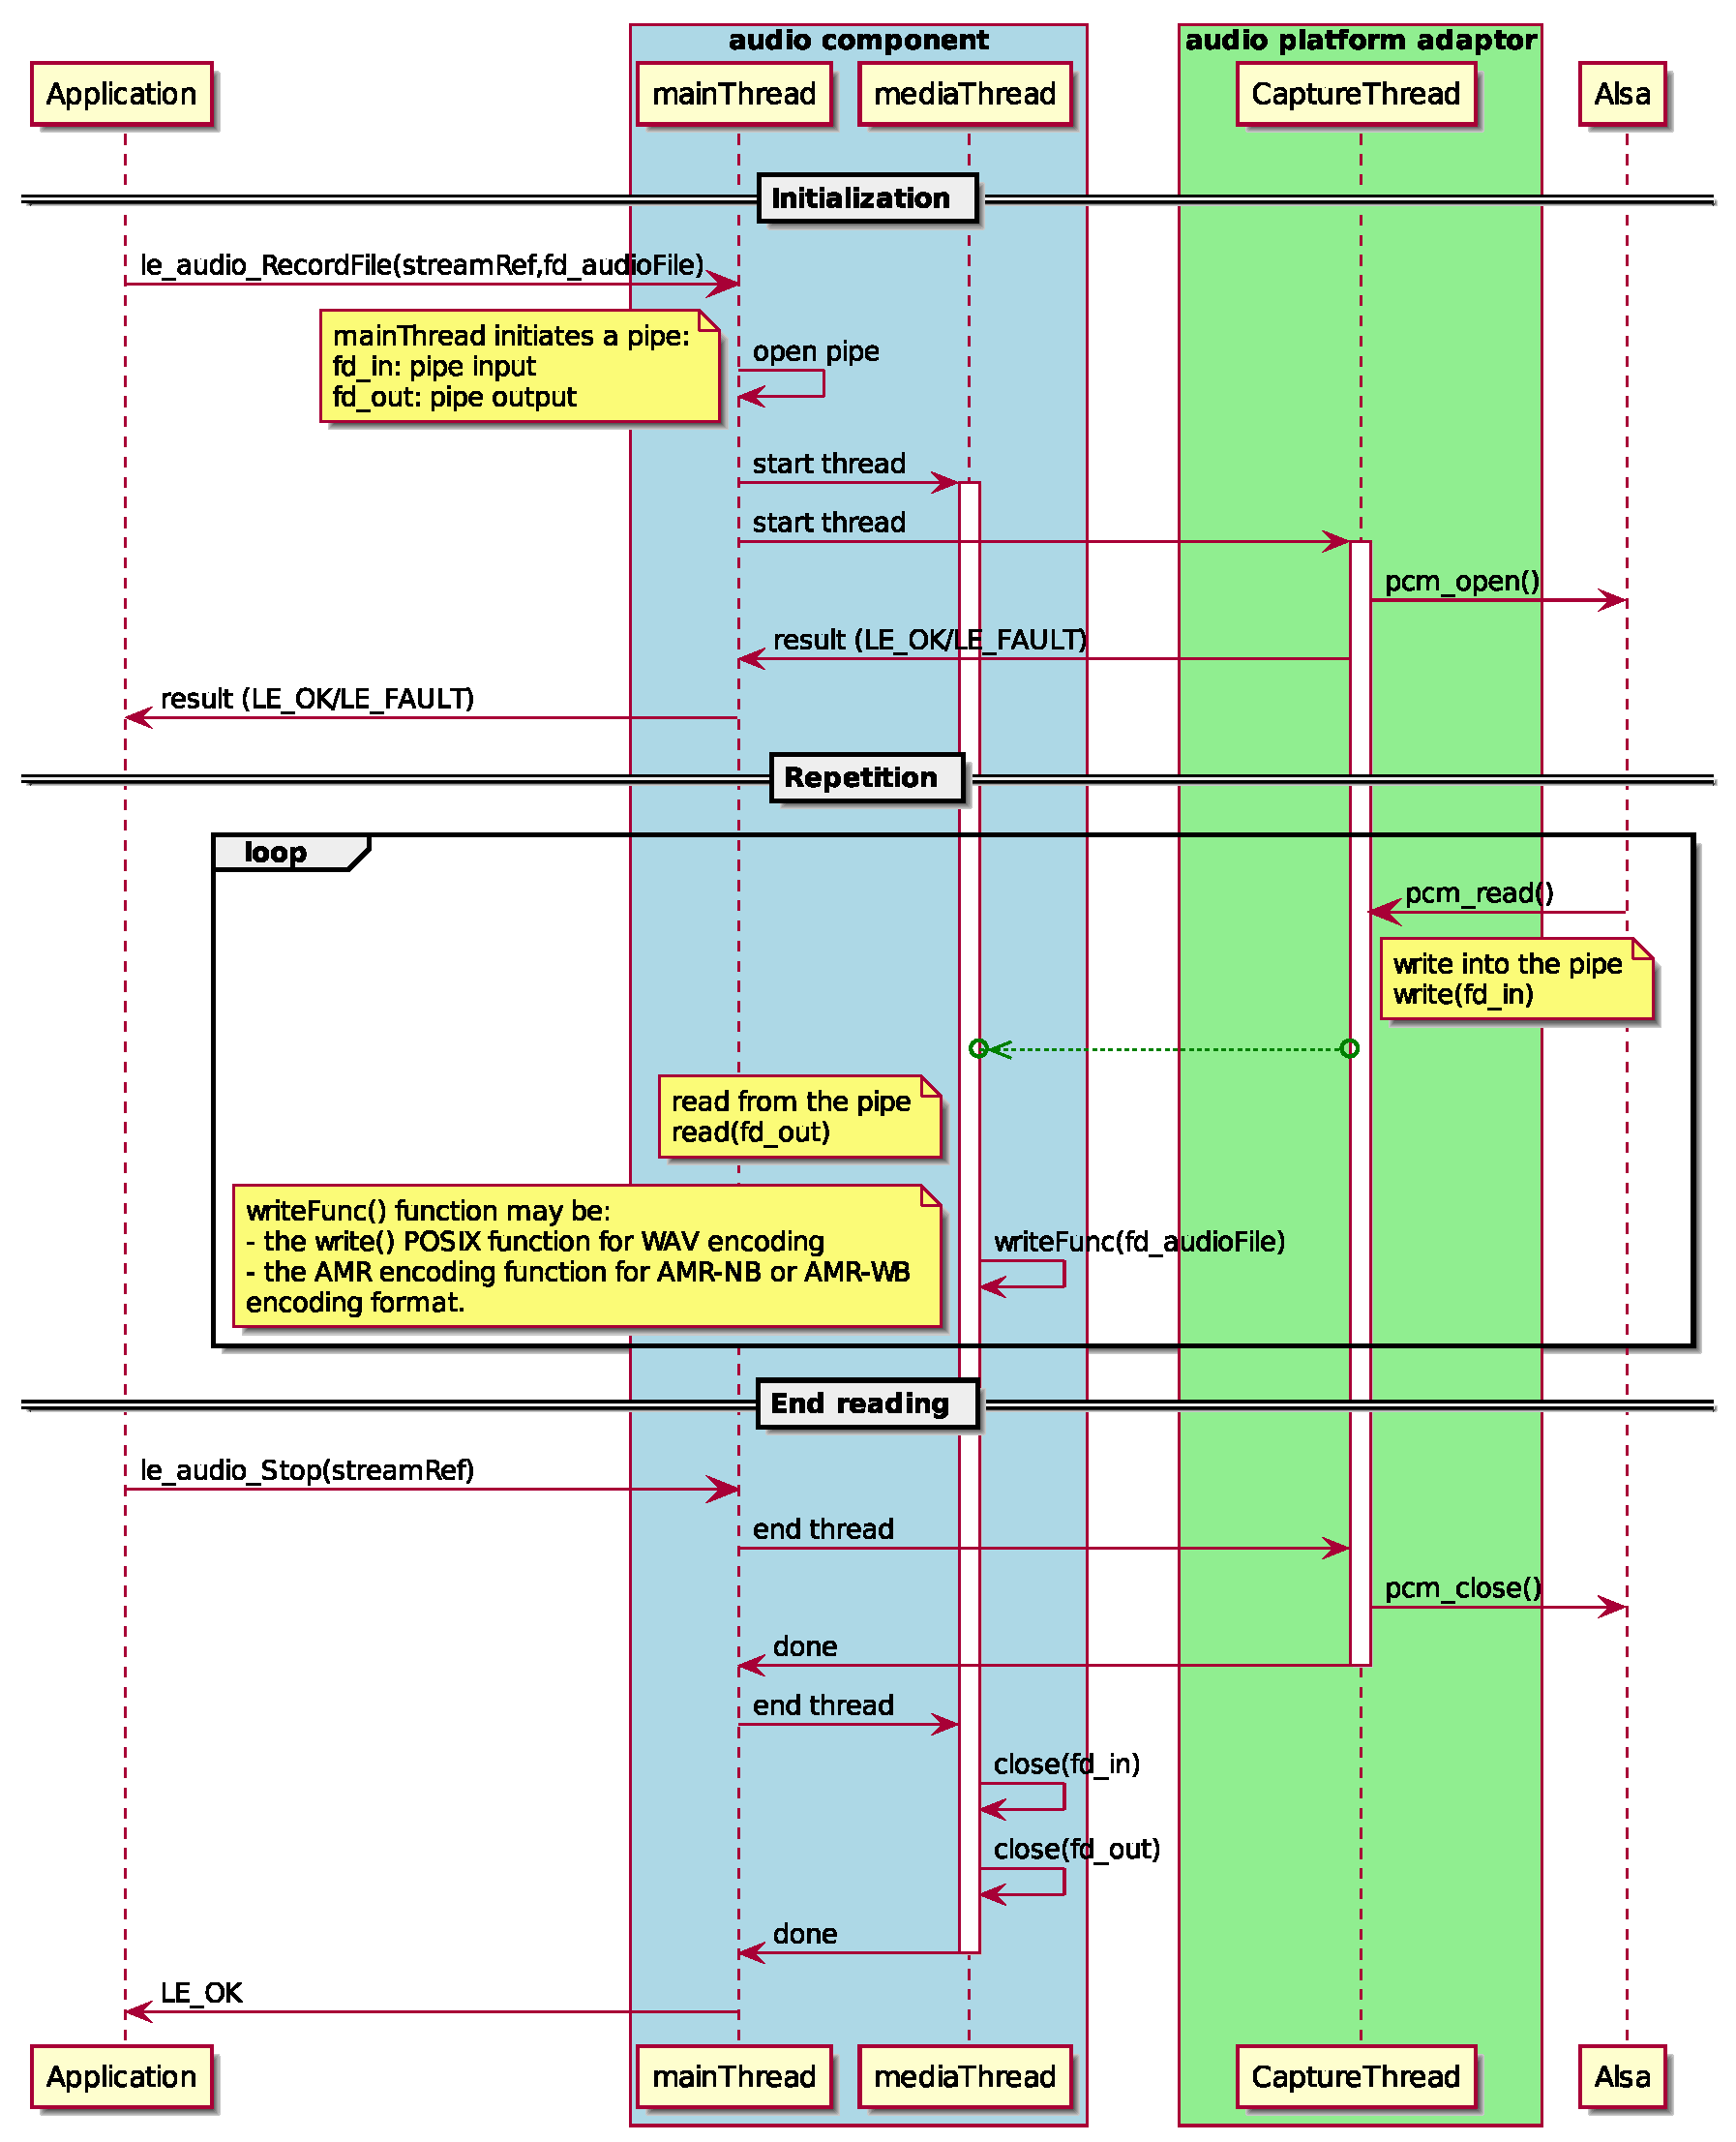
\includegraphics[width=\textwidth,height=\textheight/2,keepaspectratio=true]{le_audio_RecordFile}}
\end{DoxyImageNoCaption}


Copyright (C) Sierra Wireless Inc. \hypertarget{c_SDD_atClient}{}\section{AT client S\+DD}\label{c_SDD_atClient}
\hypertarget{c_SDD_atClient_atClient_service}{}\subsection{A\+T Client Service}\label{c_SDD_atClient_atClient_service}
\hypertarget{c_SDD_mdc_Overview}{}\subsubsection{Overview}\label{c_SDD_mdc_Overview}
The AT Client Service handles the AT commands sent to the modem on a specified serial device. It also supports getting AT command response. This service can be subscribed by several apps simultaneously.\hypertarget{c_SDD_atClient_atClient_binding}{}\subsubsection{Device Binding}\label{c_SDD_atClient_atClient_binding}
\hyperlink{le__at_client__interface_8h_a58f48ecb3c1569a4b68be4006a751f36}{le\+\_\+at\+Client\+\_\+\+Start()} must be called to bind a specific device with the AT Client. This A\+PI starts the device thread, which polls until data is available on the device. A device can be unbound using \hyperlink{le__at_client__interface_8h_a1cf248c81134ae44639ab62e3c501cf1}{le\+\_\+at\+Client\+\_\+\+Stop()}.

\hyperlink{le__at_client__interface_8h_aead1c543cd8e65d1ad531233af2c7529}{le\+\_\+at\+Client\+\_\+\+Create()} creates an AT command reference, then use \hyperlink{le__at_client__interface_8h_a156e43a17cd85dee38fb7ae4182e8864}{le\+\_\+at\+Client\+\_\+\+Set\+Command()} to set the AT command to be sent to the modem. \hyperlink{le__at_client__interface_8h_a44588125903f97d422ea14c5fd534683}{le\+\_\+at\+Client\+\_\+\+Set\+Device()} binds the command reference to the device reference.

The following sample code demonstrates how to bind AT Client with device is presented below\+: 
\begin{DoxyCodeInclude}
\textcolor{comment}{    //! [binding]}
\textcolor{comment}{}    \textcolor{keywordtype}{int} fd = open(\textcolor{stringliteral}{"/dev/ttyAT"}, O\_RDWR | O\_NOCTTY | O\_NONBLOCK);

    \hyperlink{le__log_8h_ac0dbbef91dc0fed449d0092ff0557b39}{LE\_ASSERT}(fd >= 0);

    \textcolor{keywordtype}{int} newFd = dup(fd);

    DevRef = \hyperlink{le__at_client__interface_8h_a58f48ecb3c1569a4b68be4006a751f36}{le\_atClient\_Start}(fd);\textcolor{comment}{}
\textcolor{comment}{    //! [binding]}
\textcolor{comment}{}
    \textcolor{comment}{// Try to stop the device}
    \hyperlink{le__log_8h_ac0dbbef91dc0fed449d0092ff0557b39}{LE\_ASSERT}(\hyperlink{le__at_client__interface_8h_a1cf248c81134ae44639ab62e3c501cf1}{le\_atClient\_Stop}(DevRef) == LE\_OK);
    \hyperlink{le__log_8h_ac0dbbef91dc0fed449d0092ff0557b39}{LE\_ASSERT}(\hyperlink{le__at_client__interface_8h_a1cf248c81134ae44639ab62e3c501cf1}{le\_atClient\_Stop}(DevRef) == \hyperlink{le__basics_8h_a1cca095ed6ebab24b57a636382a6c86cac409634423b6b1ef09643529f6224798}{LE\_FAULT});

    DevRef = \hyperlink{le__at_client__interface_8h_a58f48ecb3c1569a4b68be4006a751f36}{le\_atClient\_Start}(newFd);

    newThreadPtr = \hyperlink{le__thread_8h_a87e02a46f92e9e3e11ed28a2b265872f}{le\_thread\_Create}(\textcolor{stringliteral}{"TestThread"},TestThread,NULL);

    \hyperlink{le__thread_8h_a38df3877ee5ab9fac17b2fc0be46c27e}{le\_thread\_Start}(newThreadPtr);

    \textcolor{keywordtype}{char} buffer[\hyperlink{le__at_defs__interface_8h_acbaa10c00b1ff1250d2b7338225ea9ea}{LE\_ATDEFS\_RESPONSE\_MAX\_BYTES}];
    \hyperlink{le__at_client__interface_8h_ab12f48d1655a83a00bd4b2026318a6ad}{le\_atClient\_CmdRef\_t} cmdRef;

    \textcolor{comment}{// Get S/N}
    cmdRef = \hyperlink{le__at_client__interface_8h_aead1c543cd8e65d1ad531233af2c7529}{le\_atClient\_Create}();
    \hyperlink{le__log_8h_ac0dbbef91dc0fed449d0092ff0557b39}{LE\_ASSERT}(\hyperlink{le__at_client__interface_8h_a44588125903f97d422ea14c5fd534683}{le\_atClient\_SetDevice}(cmdRef, DevRef) == LE\_OK);
    \hyperlink{le__log_8h_ac0dbbef91dc0fed449d0092ff0557b39}{LE\_ASSERT}(\hyperlink{le__at_client__interface_8h_a156e43a17cd85dee38fb7ae4182e8864}{le\_atClient\_SetCommand}(cmdRef, \textcolor{stringliteral}{"AT+CGSN"}) == LE\_OK);
    \hyperlink{le__log_8h_ac0dbbef91dc0fed449d0092ff0557b39}{LE\_ASSERT}(\hyperlink{le__at_client__interface_8h_a99062518237b59b56faf45f8511419e9}{le\_atClient\_SetFinalResponse}(cmdRef, \textcolor{stringliteral}{"OK|ERROR|+CME
       ERROR"}) == LE\_OK);
\end{DoxyCodeInclude}
 The final response of AT command can be set with \hyperlink{le__at_client__interface_8h_a99062518237b59b56faf45f8511419e9}{le\+\_\+at\+Client\+\_\+\+Set\+Final\+Response()}. If an AT command answers with a final response that does not belong to the final responses set, the AT command execution should end by timeout. The timeout can be set with \hyperlink{le__at_client__interface_8h_ae6cabb33a5093aeab2019f12dde27bdb}{le\+\_\+at\+Client\+\_\+\+Set\+Timeout()}, default value is 30s.

The following sample code demonstrates how to set timeout and final response for AT command\+: 
\begin{DoxyCodeInclude}
    \textcolor{comment}{// Send a SMS}
    \textcolor{keywordtype}{char} cmgs[100];
    memset(cmgs,0,100);
    \hyperlink{app_stop_client_8c_a2b6c4b2a795957a91039524b524be480}{snprintf}(cmgs,100,\textcolor{stringliteral}{"AT+CMGS=\(\backslash\)"%s\(\backslash\)""}, phoneNumber);

    cmdRef = \hyperlink{le__at_client__interface_8h_aead1c543cd8e65d1ad531233af2c7529}{le\_atClient\_Create}();
    \hyperlink{le__log_8h_ac0dbbef91dc0fed449d0092ff0557b39}{LE\_ASSERT}(cmdRef != NULL);
    \hyperlink{le__log_8h_ac0dbbef91dc0fed449d0092ff0557b39}{LE\_ASSERT}(\hyperlink{le__at_client__interface_8h_a156e43a17cd85dee38fb7ae4182e8864}{le\_atClient\_SetCommand}(cmdRef, cmgs) == LE\_OK);
    \textcolor{keywordtype}{char} sms[]=\textcolor{stringliteral}{"Hello Legato"};
    \hyperlink{le__log_8h_ac0dbbef91dc0fed449d0092ff0557b39}{LE\_ASSERT}(\hyperlink{le__at_client__interface_8h_a45435484c7242dc301cec60417d047b7}{le\_atClient\_SetText}(cmdRef, sms) == LE\_OK);
    \hyperlink{le__log_8h_ac0dbbef91dc0fed449d0092ff0557b39}{LE\_ASSERT}(\hyperlink{le__at_client__interface_8h_a44588125903f97d422ea14c5fd534683}{le\_atClient\_SetDevice}(cmdRef, DevRef) == LE\_OK);
    \hyperlink{le__log_8h_ac0dbbef91dc0fed449d0092ff0557b39}{LE\_ASSERT}(\hyperlink{le__at_client__interface_8h_ae6cabb33a5093aeab2019f12dde27bdb}{le\_atClient\_SetTimeout}(cmdRef, 0) == LE\_OK);
    \hyperlink{le__log_8h_ac0dbbef91dc0fed449d0092ff0557b39}{LE\_ASSERT}(\hyperlink{le__at_client__interface_8h_a99062518237b59b56faf45f8511419e9}{le\_atClient\_SetFinalResponse}(cmdRef, \textcolor{stringliteral}{"OK|ERROR|+CMS
       ERROR"}) == LE\_OK);
    \hyperlink{le__log_8h_ac0dbbef91dc0fed449d0092ff0557b39}{LE\_ASSERT}(\hyperlink{le__at_client__interface_8h_aaf39cf9ae5ffb4c76a6eefc8be030e7c}{le\_atClient\_Send}(cmdRef)==LE\_OK);
\end{DoxyCodeInclude}
 When the AT command declaration is complete, it can be sent using \hyperlink{le__at_client__interface_8h_aaf39cf9ae5ffb4c76a6eefc8be030e7c}{le\+\_\+at\+Client\+\_\+\+Send()}. This A\+PI is synchronous (blocking until final response is detected, or time out reached).\hypertarget{c_SDD_atClient_atClient_state_machines}{}\subsubsection{State Machines}\label{c_SDD_atClient_atClient_state_machines}
There are two finite state machines, AT command client state machine and Rx parser state machine. The AT command client state machine takes care of writing of AT command onto modem device and Rx parser state machine looks for the response message from the modem device for the AT Command sent by client.

The following diagram describes the client state machine\+:


\begin{DoxyImageNoCaption}
  \mbox{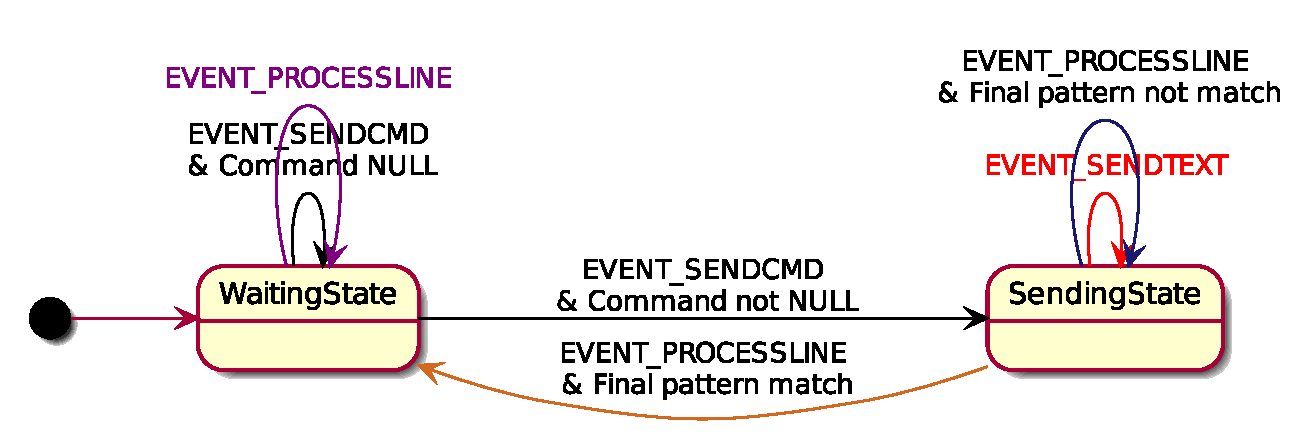
\includegraphics[width=\textwidth,height=\textheight/2,keepaspectratio=true]{client_state_machine}}
\end{DoxyImageNoCaption}


The following diagram describes the Rx parser state machine\+:


\begin{DoxyImageNoCaption}
  \mbox{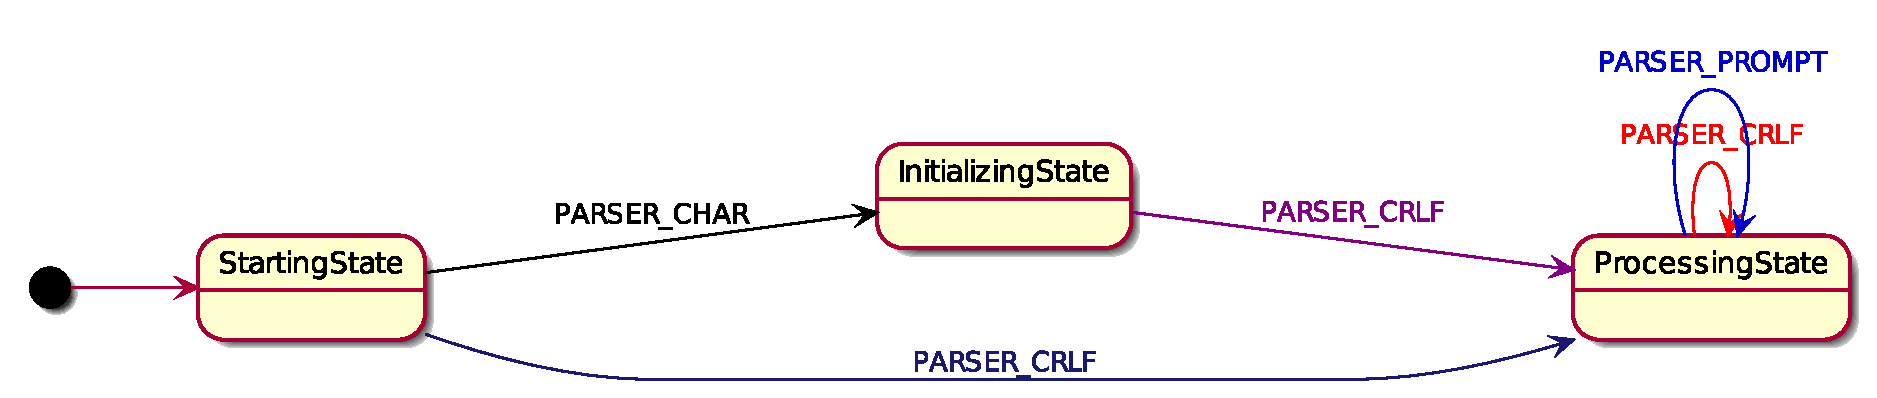
\includegraphics[width=\textwidth,height=\textheight/2,keepaspectratio=true]{Rx_parser_state_machine}}
\end{DoxyImageNoCaption}
\hypertarget{c_SDD_atClient_atClient_send}{}\subsubsection{Sending}\label{c_SDD_atClient_atClient_send}
\hyperlink{le__at_client__interface_8h_aaf39cf9ae5ffb4c76a6eefc8be030e7c}{le\+\_\+at\+Client\+\_\+\+Send()} changes the client state from Waiting\+State to Sending\+State. In the Sending\+State the AT command is written on to the device by le\+\_\+dev\+\_\+write(). The reply for the AT command is received by Rx\+New\+Data(). Rx\+New\+Data() invokes Parse\+Rx\+Buffer(), which is responsible for state change in the Rx parser state machine.

Processing\+State sends the final reponse found from the device to the client with event E\+V\+E\+N\+T\+\_\+\+P\+R\+O\+C\+E\+S\+S\+L\+I\+NE.

Sending\+State checks if the response matches with the final string of the command using the Check\+Response(). After checking response, Rx\+New\+Data() resets Rx buffer which is already read. Client state changes to Waiting\+State where as Rx parser state waits in Processing\+State.\hypertarget{c_SDD_atClient_atClient__delete}{}\subsubsection{Deleting}\label{c_SDD_atClient_atClient__delete}
When the AT command is over, the reference has to be deleted by calling \hyperlink{le__at_client__interface_8h_a8bd3f6ec64a7a700460e4d66b39ec4ed}{le\+\_\+at\+Client\+\_\+\+Delete()}.

The following flow diagram describes the AT Client Service\+:


\begin{DoxyImageNoCaption}
  \mbox{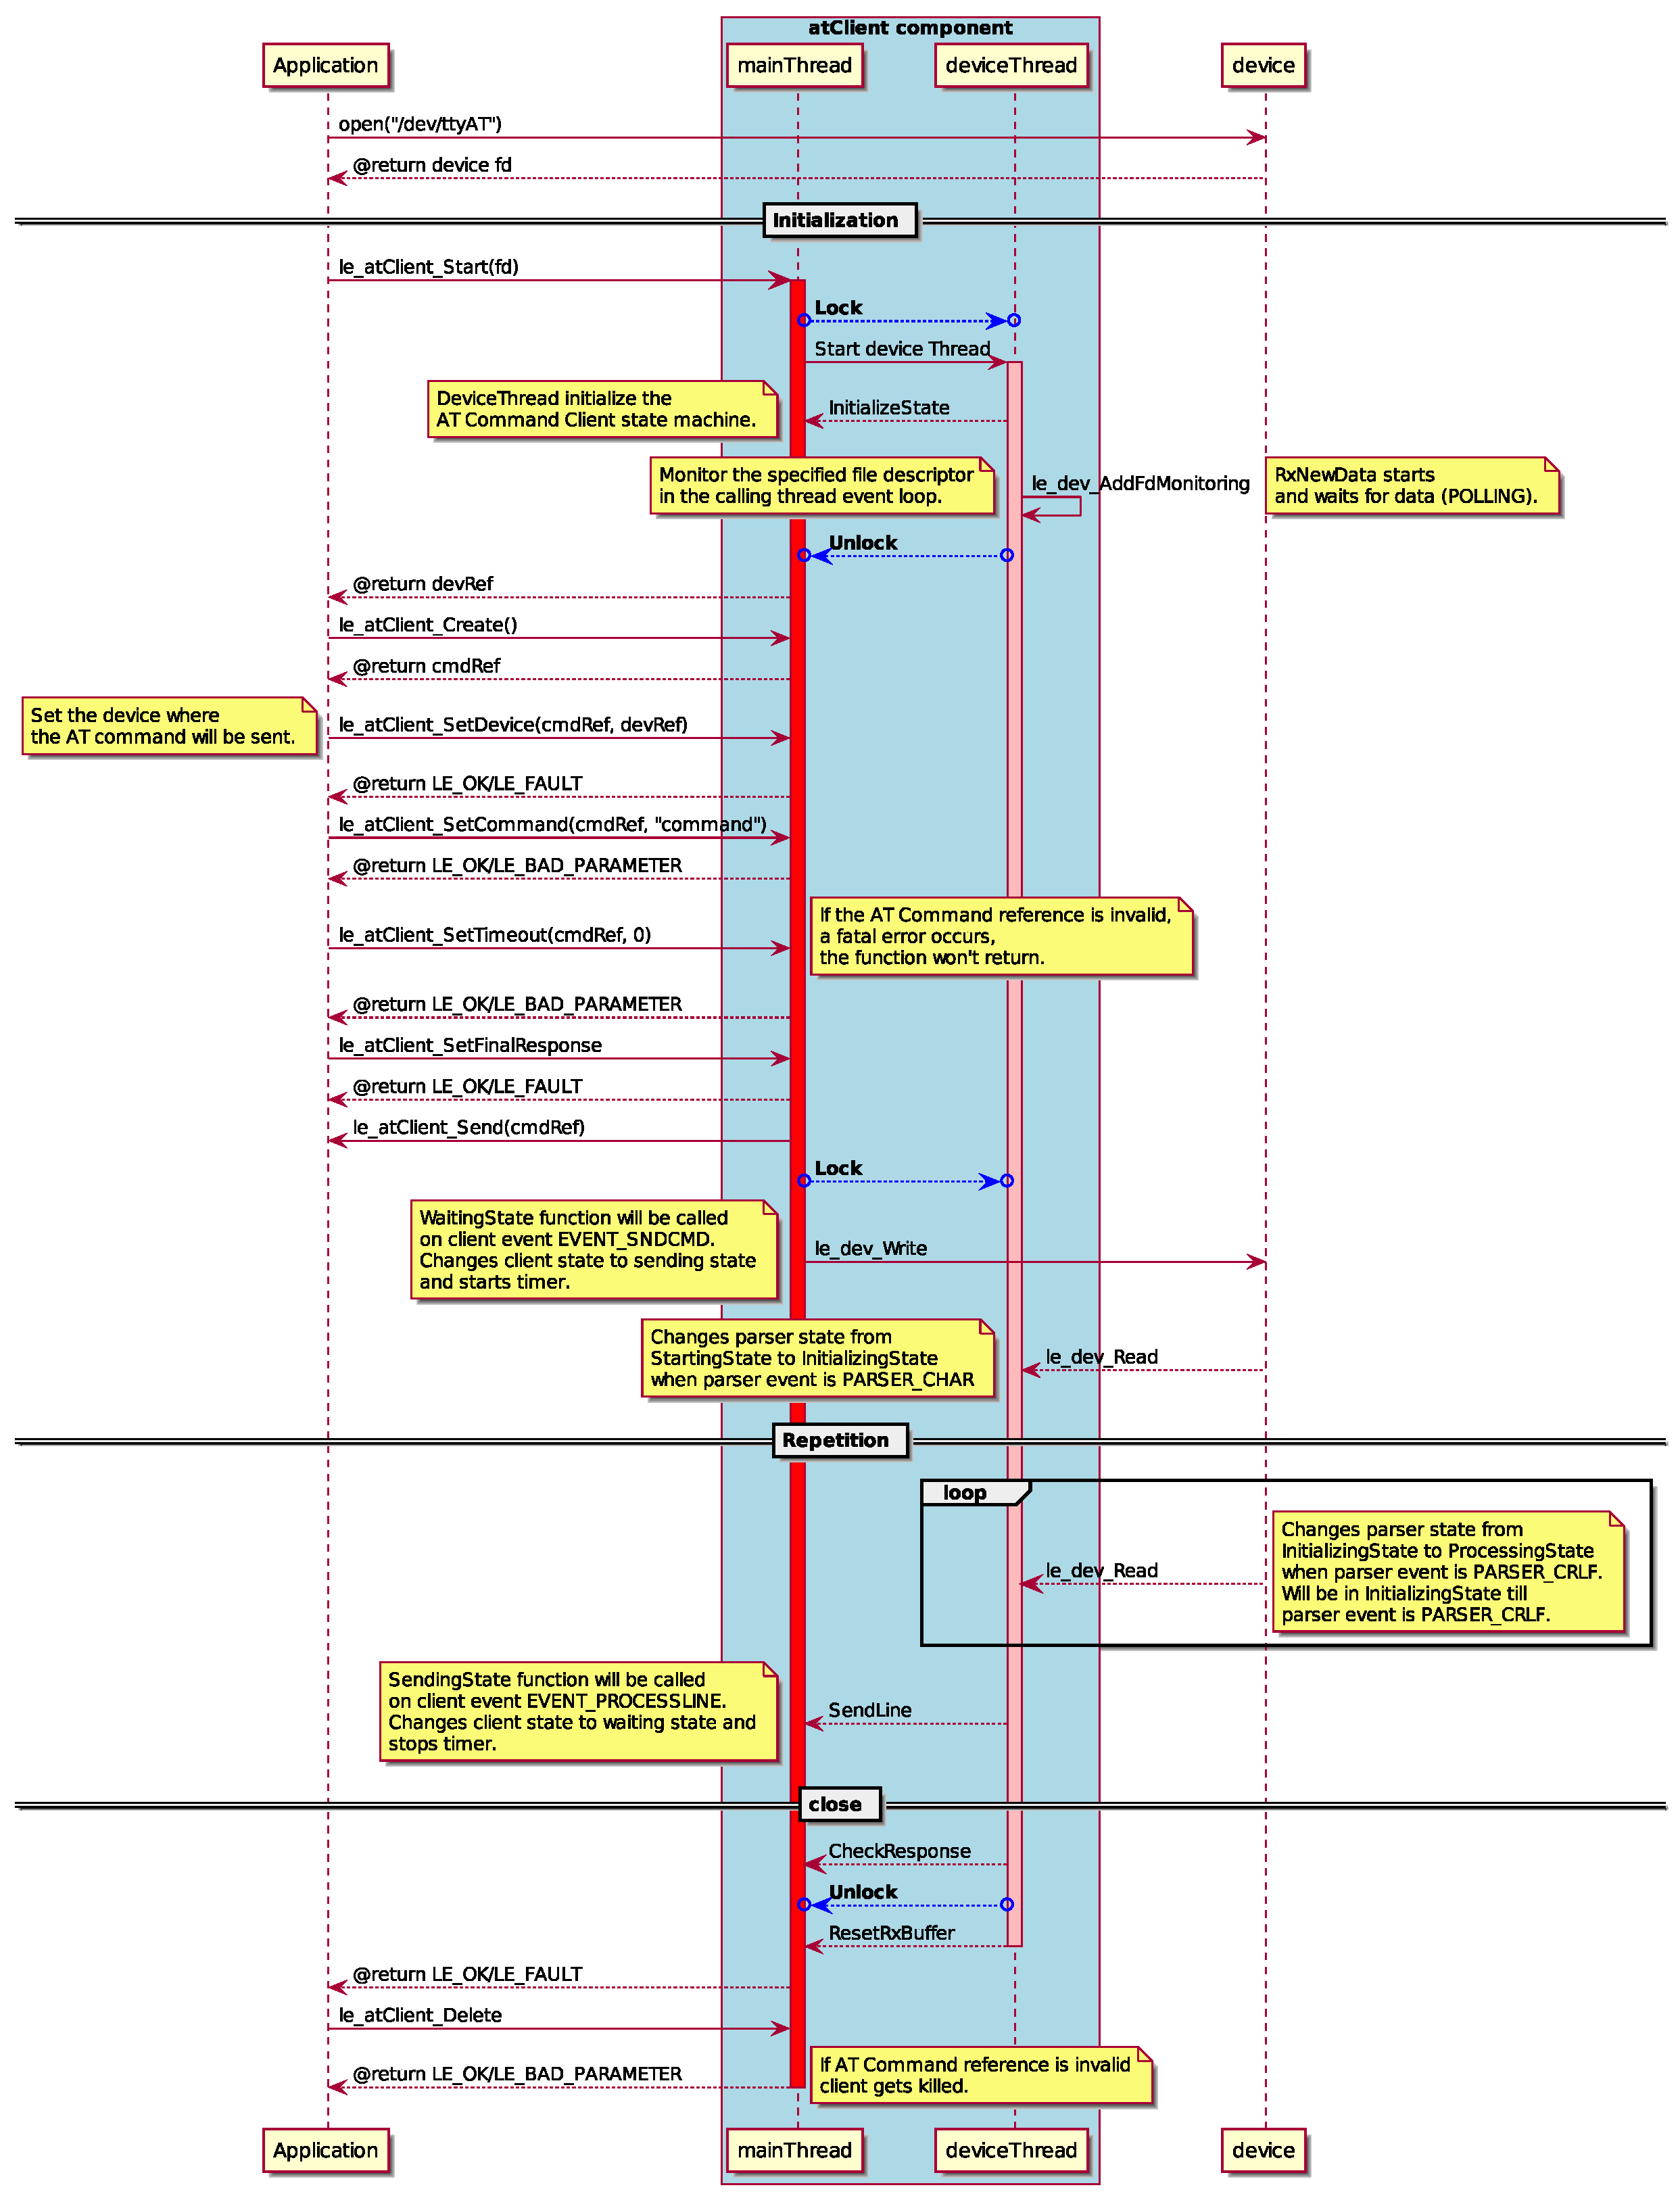
\includegraphics[width=\textwidth,height=\textheight/2,keepaspectratio=true]{le_atClient}}
\end{DoxyImageNoCaption}


Copyright (C) Sierra Wireless Inc. \hypertarget{c_SDD_mdc}{}\section{Modem Data Control S\+DD}\label{c_SDD_mdc}
\hypertarget{c_SDD_mdc_mdc_service}{}\subsection{M\+D\+C Service}\label{c_SDD_mdc_mdc_service}
\hypertarget{c_SDD_mdc_Overview}{}\subsubsection{Overview}\label{c_SDD_mdc_Overview}
A data session is useful for applications that need to send or receive data over a network. To start a data session, a data profile must be configured as specified by the target network.

The Modem Data Control (M\+DC) A\+PI is used to manage data profiles and data sessions.\hypertarget{c_SDD_mdc_mdc_dataProfile}{}\subsubsection{Data profiles}\label{c_SDD_mdc_mdc_dataProfile}
If a pre-\/defined data profile has been configured then this profile can be loaded using \hyperlink{le__mdc__interface_8h_a638b693cd5f644fa5c24f81e1e36483c}{le\+\_\+mdc\+\_\+\+Get\+Profile()}. \hyperlink{le__mdc__interface_8h_a638b693cd5f644fa5c24f81e1e36483c}{le\+\_\+mdc\+\_\+\+Get\+Profile()} must be called with L\+E\+\_\+\+M\+D\+C\+\_\+\+D\+E\+F\+A\+U\+L\+T\+\_\+\+P\+R\+O\+F\+I\+LE to retrieve the default index used by the modem for data connection. \hyperlink{le__mdc__interface_8h_a638b693cd5f644fa5c24f81e1e36483c}{le\+\_\+mdc\+\_\+\+Get\+Profile()} must be called with L\+E\+\_\+\+M\+D\+C\+\_\+\+S\+I\+M\+T\+O\+O\+L\+K\+I\+T\+\_\+\+B\+I\+P\+\_\+\+D\+E\+F\+A\+U\+L\+T\+\_\+\+P\+R\+O\+F\+I\+LE to retrieve the default index used by the modem for Bearer Independent Protocol (B\+IP).

\begin{DoxyWarning}{Warning}
0 is not a valid index.
\end{DoxyWarning}
The following data profile parameters can be retrieved\+: \begin{DoxyVerb}Packet Data Protocol using le_mdc_GetPDP().
Access Point Name using le_mdc_GetAPN().
Authentication settings using le_mdc_GetAuthentication().
\end{DoxyVerb}


The following data profile parameters can be set\+: \begin{DoxyVerb}Packet Data Protocol using le_mdc_SetPDP().
Access Point Name using le_mdc_SetAPN().
Authentication settings using le_mdc_SetAuthentication().
\end{DoxyVerb}


The following sample code demonstrates data profile parameters\+: 
\begin{DoxyCodeInclude}

    \textcolor{comment}{// Get the profile reference}
    *profileRefPtr = \hyperlink{le__mdc__interface_8h_a638b693cd5f644fa5c24f81e1e36483c}{le\_mdc\_GetProfile}(profile);
    \hyperlink{le__log_8h_ac0dbbef91dc0fed449d0092ff0557b39}{LE\_ASSERT}(NULL != *profileRefPtr);

    \textcolor{comment}{// Check the current state of the cid}
    \hyperlink{le__mdc__interface_8h_a0727e543d0394422963c8d6297947333}{le\_mdc\_ConState\_t} state = \hyperlink{le__mdc__interface_8h_a0727e543d0394422963c8d6297947333a6d11ee963528c79d73a269eb85202ba7}{LE\_MDC\_DISCONNECTED};

    \textcolor{comment}{// Check the state}
    \hyperlink{le__log_8h_ac0dbbef91dc0fed449d0092ff0557b39}{LE\_ASSERT}(LE\_OK == \hyperlink{le__mdc__interface_8h_add91c364e8b3e4e82a0ce64e480c016b}{le\_mdc\_GetSessionState}(*profileRefPtr, &state));

    \textcolor{comment}{// If already connected, disconnect the session}
    \textcolor{keywordflow}{if} (\hyperlink{le__mdc__interface_8h_a0727e543d0394422963c8d6297947333a0a8a2113935b881b76c59b94cf7223b8}{LE\_MDC\_CONNECTED} == state)
    \{
        \hyperlink{le__log_8h_ac0dbbef91dc0fed449d0092ff0557b39}{LE\_ASSERT}(\hyperlink{le__mdc__interface_8h_a53453f85065c3cace0922150b7e3d869}{le\_mdc\_StopSession}(*profileRefPtr) == LE\_OK);
    \}

    \textcolor{comment}{// Set pdp type}
    \hyperlink{le__mdc__interface_8h_a85721ec6046140c2f87c23f877dce247}{le\_mdc\_Pdp\_t} pdp = \hyperlink{le__mdc__interface_8h_a85721ec6046140c2f87c23f877dce247a590fd5c933c3751e42053f996d530987}{LE\_MDC\_PDP\_UNKNOWN};

    \textcolor{keywordflow}{if} (0 == strncmp(configuration.pdp, PdpIpv4, \textcolor{keyword}{sizeof}(PdpIpv4)))
    \{
        pdp = \hyperlink{le__mdc__interface_8h_a85721ec6046140c2f87c23f877dce247af550adf5bcecb680294f92f28496a830}{LE\_MDC\_PDP\_IPV4};
    \}
    \textcolor{keywordflow}{else} \textcolor{keywordflow}{if} (0 == strncmp(configuration.pdp, PdpIpv6, \textcolor{keyword}{sizeof}(PdpIpv6)))
    \{
        pdp = \hyperlink{le__mdc__interface_8h_a85721ec6046140c2f87c23f877dce247ac2d2a34bad2d18be1ea8facef0effad0}{LE\_MDC\_PDP\_IPV6};
    \}
    \textcolor{keywordflow}{else} \textcolor{keywordflow}{if} (0 == strncmp(configuration.pdp, PdpIpv4v6, \textcolor{keyword}{sizeof}(PdpIpv4v6)))
    \{
        pdp = \hyperlink{le__mdc__interface_8h_a85721ec6046140c2f87c23f877dce247a4427db8ba7a89ebf66c7b62eacfc8275}{LE\_MDC\_PDP\_IPV4V6};
    \}

    \hyperlink{le__log_8h_ac0dbbef91dc0fed449d0092ff0557b39}{LE\_ASSERT}(LE\_OK == \hyperlink{le__mdc__interface_8h_a73e66a7a63dc95d7f261fc2a26470386}{le\_mdc\_SetPDP}(*profileRefPtr, pdp));

    \textcolor{comment}{// Set APN}
    \textcolor{keywordflow}{if} (0 == strncmp(configuration.apn, automaticApn, \textcolor{keyword}{sizeof}(automaticApn)))
    \{
        \textcolor{comment}{// Set default APN}
        \hyperlink{le__log_8h_ac0dbbef91dc0fed449d0092ff0557b39}{LE\_ASSERT}(LE\_OK == \hyperlink{le__mdc__interface_8h_ad44bd756fd5cbfd43a5b348054786a4d}{le\_mdc\_SetDefaultAPN}(*profileRefPtr));
    \}
    \textcolor{keywordflow}{else}
    \{
        \hyperlink{le__log_8h_ac0dbbef91dc0fed449d0092ff0557b39}{LE\_ASSERT}(LE\_OK == \hyperlink{le__mdc__interface_8h_ae8ebd11b9cb9afb9b6b5745903f50156}{le\_mdc\_SetAPN}(*profileRefPtr, configuration.apn));
    \}

    \hyperlink{le__mdc__interface_8h_ae9758eecfab89fbc1bc01341393a7723}{le\_mdc\_Auth\_t} auth = \hyperlink{le__mdc__interface_8h_ae9758eecfab89fbc1bc01341393a7723a10fb016f4d6f7a7e893cf66846c24de2}{LE\_MDC\_AUTH\_NONE};
    \textcolor{keywordflow}{if} (\textcolor{charliteral}{'\(\backslash\)0'} != configuration.auth[0])
    \{
        \textcolor{comment}{// Set the authentication, username and password}
        \textcolor{keywordflow}{if} (0 == strncmp(configuration.auth, AuthPapChap, \textcolor{keyword}{sizeof}(AuthPapChap)))
        \{
            auth = \hyperlink{le__mdc__interface_8h_ae9758eecfab89fbc1bc01341393a7723a151065be441aa8f065d0ead3d739b6f0}{LE\_MDC\_AUTH\_PAP} | \hyperlink{le__mdc__interface_8h_ae9758eecfab89fbc1bc01341393a7723ae93a464a7ee2f31346aa01676afc7054}{LE\_MDC\_AUTH\_CHAP};
        \}
        \textcolor{comment}{// Set the authentication, username and password}
        \textcolor{keywordflow}{else} \textcolor{keywordflow}{if} (0 == strncmp(configuration.auth, AuthPap, \textcolor{keyword}{sizeof}(AuthPap)))
        \{
            auth = \hyperlink{le__mdc__interface_8h_ae9758eecfab89fbc1bc01341393a7723a151065be441aa8f065d0ead3d739b6f0}{LE\_MDC\_AUTH\_PAP};
        \}
        \textcolor{keywordflow}{else} \textcolor{keywordflow}{if} (0 == strncmp(configuration.auth, AuthChap, \textcolor{keyword}{sizeof}(AuthChap)))
        \{
            auth = \hyperlink{le__mdc__interface_8h_ae9758eecfab89fbc1bc01341393a7723ae93a464a7ee2f31346aa01676afc7054}{LE\_MDC\_AUTH\_CHAP};
        \}

        \textcolor{keywordflow}{if} (\hyperlink{le__mdc__interface_8h_ae9758eecfab89fbc1bc01341393a7723a10fb016f4d6f7a7e893cf66846c24de2}{LE\_MDC\_AUTH\_NONE} != auth)
        \{
            \hyperlink{le__log_8h_ac0dbbef91dc0fed449d0092ff0557b39}{LE\_ASSERT}(LE\_OK == \hyperlink{le__mdc__interface_8h_a9f69d0751927b5ead6c756202179b222}{le\_mdc\_SetAuthentication}(*profileRefPtr,
                                                auth,
                                                configuration.userName,
                                                configuration.password));
        \}
    \}

    \hyperlink{le__log_8h_a23e6d206faa64f612045d688cdde5808}{LE\_INFO}(\textcolor{stringliteral}{"cid: %d pdp: %d apn: %s auth: %d username: %s password: %s"},
            \hyperlink{le__mdc__interface_8h_a108f7c3db74a377c2ae5482543d4e0d9}{le\_mdc\_GetProfileIndex}(*profileRefPtr), pdp, configuration.apn, auth,
            configuration.userName, configuration.password);
\}\textcolor{comment}{}
\textcolor{comment}{//! [Profiles]}
\end{DoxyCodeInclude}
 \hypertarget{c_SDD_mdc_mdc_StartSession}{}\subsubsection{Start Data Session}\label{c_SDD_mdc_mdc_StartSession}
A data session can be started using \hyperlink{le__mdc__interface_8h_a2cb08d5c3e6c43297d80448891719649}{le\+\_\+mdc\+\_\+\+Start\+Session()}. To start a data session, a data profile must be created and written to the modem, or an existing data profile can be used. The number of simultaneous data sessions supported is dependent on the modem, but cannot be more than the maximum number of supported profiles.

A data session can be started asynchronously using \hyperlink{le__mdc__interface_8h_aa03d6e31263ddf8bf1d94b183c9934d9}{le\+\_\+mdc\+\_\+\+Start\+Session\+Async()}, which is not blocking. The response will be returned with the le\+\_\+mdc\+\_\+\+Session\+Handler\+Func\+\_\+t handler function.

When \hyperlink{le__mdc__interface_8h_a638b693cd5f644fa5c24f81e1e36483c}{le\+\_\+mdc\+\_\+\+Get\+Profile()} called with L\+E\+\_\+\+M\+D\+C\+\_\+\+D\+E\+F\+A\+U\+L\+T\+\_\+\+P\+R\+O\+F\+I\+LE, profile index 1(default index) is retrieved from the modem. To register with another profile other than L\+E\+\_\+\+M\+D\+C\+\_\+\+D\+E\+F\+A\+U\+L\+T\+\_\+\+P\+R\+O\+F\+I\+LE, the required profile index should be passed to \hyperlink{le__mdc__interface_8h_a638b693cd5f644fa5c24f81e1e36483c}{le\+\_\+mdc\+\_\+\+Get\+Profile()}.

\begin{DoxyNote}{Note}
\+: The maximum number of data profiles supported is modem dependent and can be retrieved with \hyperlink{le__mdc__interface_8h_a790602f1b17d7bf9626a51eac5599439}{le\+\_\+mdc\+\_\+\+Num\+Profiles()}. Profile index passed to le\+\_\+mdc\+\_\+\+Get\+Profile(profile\+\_\+index) should be less than or equal to maximum number of data profiles supported.
\end{DoxyNote}
\hypertarget{c_SDD_mdc_mdc_StopSession}{}\subsubsection{Stop Data Session}\label{c_SDD_mdc_mdc_StopSession}
A data session can be stopped using \hyperlink{le__mdc__interface_8h_a53453f85065c3cace0922150b7e3d869}{le\+\_\+mdc\+\_\+\+Stop\+Session()}.

A data session started can be stopped either synchronously with \hyperlink{le__mdc__interface_8h_a53453f85065c3cace0922150b7e3d869}{le\+\_\+mdc\+\_\+\+Stop\+Session()} (or) asynchronously with \hyperlink{le__mdc__interface_8h_ac5b357f7437c9e253fa17b2511fa14ef}{le\+\_\+mdc\+\_\+\+Stop\+Session\+Async()}. \hyperlink{le__mdc__interface_8h_ac5b357f7437c9e253fa17b2511fa14ef}{le\+\_\+mdc\+\_\+\+Stop\+Session\+Async()} response will be returned with the le\+\_\+mdc\+\_\+\+Session\+Handler\+Func\+\_\+t handler function.

The following sample code demonstrates Data Session Functionality\+: 
\begin{DoxyCodeInclude}
\textcolor{comment}{//--------------------------------------------------------------------------------------------------}\textcolor{comment}{}
\textcolor{comment}{/**}
\textcolor{comment}{ * Session handler response for connection and disconnection.}
\textcolor{comment}{ */}
\textcolor{comment}{//--------------------------------------------------------------------------------------------------}
\textcolor{keyword}{static} \textcolor{keywordtype}{void} SessionHandlerFunc
(
    \hyperlink{le__mdc__interface_8h_a91074d8f0d88c6645e3085dfadf87011}{le\_mdc\_ProfileRef\_t} profileRef,
    \hyperlink{le__basics_8h_a1cca095ed6ebab24b57a636382a6c86c}{le\_result\_t} result,
    \textcolor{keywordtype}{void}* contextPtr
)
\{
    \hyperlink{le__basics_8h_a1cca095ed6ebab24b57a636382a6c86c}{le\_result\_t}* activationPtr = contextPtr;
    *activationPtr = result;

    \hyperlink{le__log_8h_a23e6d206faa64f612045d688cdde5808}{LE\_INFO}(\textcolor{stringliteral}{"Session result %d for profile %d"}, result, 
      \hyperlink{le__mdc__interface_8h_a108f7c3db74a377c2ae5482543d4e0d9}{le\_mdc\_GetProfileIndex}(profileRef));

    \hyperlink{le__semaphore_8h_abb859411cc58fbcc576c986ef52083b2}{le\_sem\_Post}(AsyncTestSemaphore);
\}

\textcolor{comment}{//--------------------------------------------------------------------------------------------------}\textcolor{comment}{}
\textcolor{comment}{/**}
\textcolor{comment}{ * Start asynchronous session.}
\textcolor{comment}{ */}
\textcolor{comment}{//--------------------------------------------------------------------------------------------------}
\textcolor{keyword}{static} \textcolor{keywordtype}{void} SessionStartAsync
(
    \textcolor{keywordtype}{void}* param1Ptr,
    \textcolor{keywordtype}{void}* param2Ptr
)
\{
    \hyperlink{le__mdc__interface_8h_a91074d8f0d88c6645e3085dfadf87011}{le\_mdc\_ProfileRef\_t} profileRef = param1Ptr;

    \hyperlink{le__mdc__interface_8h_aa03d6e31263ddf8bf1d94b183c9934d9}{le\_mdc\_StartSessionAsync}(profileRef, SessionHandlerFunc, param2Ptr);
\}

\textcolor{comment}{//--------------------------------------------------------------------------------------------------}\textcolor{comment}{}
\textcolor{comment}{/**}
\textcolor{comment}{ * Stop asynchronous session.}
\textcolor{comment}{ */}
\textcolor{comment}{//--------------------------------------------------------------------------------------------------}
\textcolor{keyword}{static} \textcolor{keywordtype}{void} SessionStopAsync
(
    \textcolor{keywordtype}{void}* param1Ptr,
    \textcolor{keywordtype}{void}* param2Ptr
)
\{
    \hyperlink{le__mdc__interface_8h_a91074d8f0d88c6645e3085dfadf87011}{le\_mdc\_ProfileRef\_t} profileRef = param1Ptr;

    \hyperlink{le__mdc__interface_8h_ac5b357f7437c9e253fa17b2511fa14ef}{le\_mdc\_StopSessionAsync}(profileRef, SessionHandlerFunc, param2Ptr);
\}

\end{DoxyCodeInclude}
\begin{DoxyNote}{Note}
Data session started synchronously can be stopped asynchronously and vice-\/versa.
\end{DoxyNote}
\hypertarget{c_SDD_mdc_le_mdc_dataStatistics}{}\subsubsection{Data Statistics}\label{c_SDD_mdc_le_mdc_dataStatistics}
The amount of received and transmitted data can be retrieved through \hyperlink{le__mdc__interface_8h_aaad833c105f7d0ae77f18195d6739080}{le\+\_\+mdc\+\_\+\+Get\+Bytes\+Counters()}. The returned values correspond to the number of received and transmitted bytes since the last call to \hyperlink{le__mdc__interface_8h_a63636b2779d2ee6a6520ebfb2d26666c}{le\+\_\+mdc\+\_\+\+Reset\+Bytes\+Counter()}.

The data statistics collection can be started with \hyperlink{le__mdc__interface_8h_a30f390941d98c9e9c4144a5e035da3aa}{le\+\_\+mdc\+\_\+\+Start\+Bytes\+Counter()} and stopped without resetting the counters with \hyperlink{le__mdc__interface_8h_a1d6007bc8f84e5e4869af4af11b7363f}{le\+\_\+mdc\+\_\+\+Stop\+Bytes\+Counter()}.

\begin{DoxyNote}{Note}
The data statistics collection activation and the data counters are persistent even after a reboot of the platform.
\end{DoxyNote}
The following sample code demonstrates Data Statistics usage\+: 
\begin{DoxyCodeInclude}
\textcolor{comment}{//--------------------------------------------------------------------------------------------------}\textcolor{comment}{}
\textcolor{comment}{/**}
\textcolor{comment}{ * Test the connectivity.}
\textcolor{comment}{ */}
\textcolor{comment}{//--------------------------------------------------------------------------------------------------}
\textcolor{keywordtype}{void} TestConnectivity
(
    \hyperlink{le__mdc__interface_8h_a91074d8f0d88c6645e3085dfadf87011}{le\_mdc\_ProfileRef\_t} profileRef
)
\{
    \textcolor{keywordtype}{int} status;
    \textcolor{keywordtype}{char} systemCmd[200] = \{0\};
    \textcolor{keywordtype}{char} itfName[\hyperlink{le__mdc__interface_8h_a33ebf9afd03f0ffc91a80c32c15afb42}{LE\_MDC\_INTERFACE\_NAME\_MAX\_BYTES}] = \textcolor{stringliteral}{"\(\backslash\)0"};
    \hyperlink{le__mdc__interface_8h_a7a9d8c4b2053b048a53257ed810f527e}{le\_mdc\_DataBearerTechnology\_t} downlinkDataBearerTech;
    \hyperlink{le__mdc__interface_8h_a7a9d8c4b2053b048a53257ed810f527e}{le\_mdc\_DataBearerTechnology\_t} uplinkDataBearerTech;
    uint64\_t rxBytes = 0, txBytes = 0;
    uint64\_t latestRxBytes = 0, latestTxBytes = 0;

    \hyperlink{le__log_8h_a7cd2daa3d4af1de4d29e0eed95187484}{LE\_ASSERT\_OK}(\hyperlink{le__mdc__interface_8h_a1b17bb87b347162013b5ad608cdcda2d}{le\_mdc\_GetDataBearerTechnology}(profileRef,
                                                &downlinkDataBearerTech,
                                                &uplinkDataBearerTech));

    \hyperlink{le__log_8h_a23e6d206faa64f612045d688cdde5808}{LE\_INFO}(\textcolor{stringliteral}{"downlinkDataBearerTech %d, uplinkDataBearerTech %d"},
            downlinkDataBearerTech, uplinkDataBearerTech);

    \textcolor{comment}{// Get interface name}
    \hyperlink{le__log_8h_a7cd2daa3d4af1de4d29e0eed95187484}{LE\_ASSERT\_OK}(\hyperlink{le__mdc__interface_8h_a4c22a8691d6e6a69270a7ed6ab9974af}{le\_mdc\_GetInterfaceName}(profileRef, itfName, 
      \hyperlink{le__mdc__interface_8h_a33ebf9afd03f0ffc91a80c32c15afb42}{LE\_MDC\_INTERFACE\_NAME\_MAX\_BYTES}));

    \textcolor{keywordflow}{if} (\hyperlink{le__mdc__interface_8h_aa3912e94864a6e5862e07f58b3772cba}{le\_mdc\_IsIPv4}(profileRef))
    \{
        \hyperlink{app_stop_client_8c_a2b6c4b2a795957a91039524b524be480}{snprintf}(systemCmd, \textcolor{keyword}{sizeof}(systemCmd), \textcolor{stringliteral}{"ping -c 4 www.sierrawireless.com -I %s"}, itfName);
    \}
    \textcolor{keywordflow}{else}
    \{
        \textcolor{comment}{// TODO ping6 needs raw access to socket and therefore root permissions => find a different}
        \textcolor{comment}{// way to test the connectivity}
        \hyperlink{app_stop_client_8c_a2b6c4b2a795957a91039524b524be480}{snprintf}(systemCmd, \textcolor{keyword}{sizeof}(systemCmd), \textcolor{stringliteral}{"ping6 -c 4 www.sierrawireless.com -I %s"}, itfName);
    \}

    \textcolor{comment}{// Ping to test the connectivity}
    status = system(systemCmd);
    \textcolor{keywordflow}{if} (WEXITSTATUS(status))
    \{
        \hyperlink{le__mdc__interface_8h_a53453f85065c3cace0922150b7e3d869}{le\_mdc\_StopSession}(profileRef);
    \}
    \hyperlink{le__log_8h_ac0dbbef91dc0fed449d0092ff0557b39}{LE\_ASSERT}(!WEXITSTATUS(status));

    \textcolor{comment}{// Get data counters}
    \hyperlink{le__log_8h_a7cd2daa3d4af1de4d29e0eed95187484}{LE\_ASSERT\_OK}(\hyperlink{le__mdc__interface_8h_aaad833c105f7d0ae77f18195d6739080}{le\_mdc\_GetBytesCounters}(&rxBytes, &txBytes));
    latestRxBytes = rxBytes;
    latestTxBytes = txBytes;
    \hyperlink{le__log_8h_a23e6d206faa64f612045d688cdde5808}{LE\_INFO}(\textcolor{stringliteral}{"rxBytes %"}PRIu64\textcolor{stringliteral}{", txBytes %"}PRIu64, rxBytes, txBytes);

    \textcolor{comment}{// Stop data counters and ping to test the connectivity}
    \hyperlink{le__log_8h_a7cd2daa3d4af1de4d29e0eed95187484}{LE\_ASSERT\_OK}(\hyperlink{le__mdc__interface_8h_a1d6007bc8f84e5e4869af4af11b7363f}{le\_mdc\_StopBytesCounter}());
    status = system(systemCmd);
    \textcolor{keywordflow}{if} (WEXITSTATUS(status))
    \{
        \hyperlink{le__mdc__interface_8h_a53453f85065c3cace0922150b7e3d869}{le\_mdc\_StopSession}(profileRef);
    \}
    \hyperlink{le__log_8h_ac0dbbef91dc0fed449d0092ff0557b39}{LE\_ASSERT}(!WEXITSTATUS(status));

    \textcolor{comment}{// Get data counters}
    \hyperlink{le__log_8h_a7cd2daa3d4af1de4d29e0eed95187484}{LE\_ASSERT\_OK}(\hyperlink{le__mdc__interface_8h_aaad833c105f7d0ae77f18195d6739080}{le\_mdc\_GetBytesCounters}(&rxBytes, &txBytes));
    \hyperlink{le__log_8h_a23e6d206faa64f612045d688cdde5808}{LE\_INFO}(\textcolor{stringliteral}{"rxBytes %"}PRIu64\textcolor{stringliteral}{", txBytes %"}PRIu64, rxBytes, txBytes);
    \hyperlink{le__log_8h_ac0dbbef91dc0fed449d0092ff0557b39}{LE\_ASSERT}(latestRxBytes == rxBytes);
    \hyperlink{le__log_8h_ac0dbbef91dc0fed449d0092ff0557b39}{LE\_ASSERT}(latestTxBytes == txBytes);

    \textcolor{comment}{// Start data counters}
    \hyperlink{le__log_8h_a7cd2daa3d4af1de4d29e0eed95187484}{LE\_ASSERT\_OK}(\hyperlink{le__mdc__interface_8h_a30f390941d98c9e9c4144a5e035da3aa}{le\_mdc\_StartBytesCounter}());
\}
\end{DoxyCodeInclude}


The following flow diagram describes how M\+DC data profile is retrieved\+:


\begin{DoxyImageNoCaption}
  \mbox{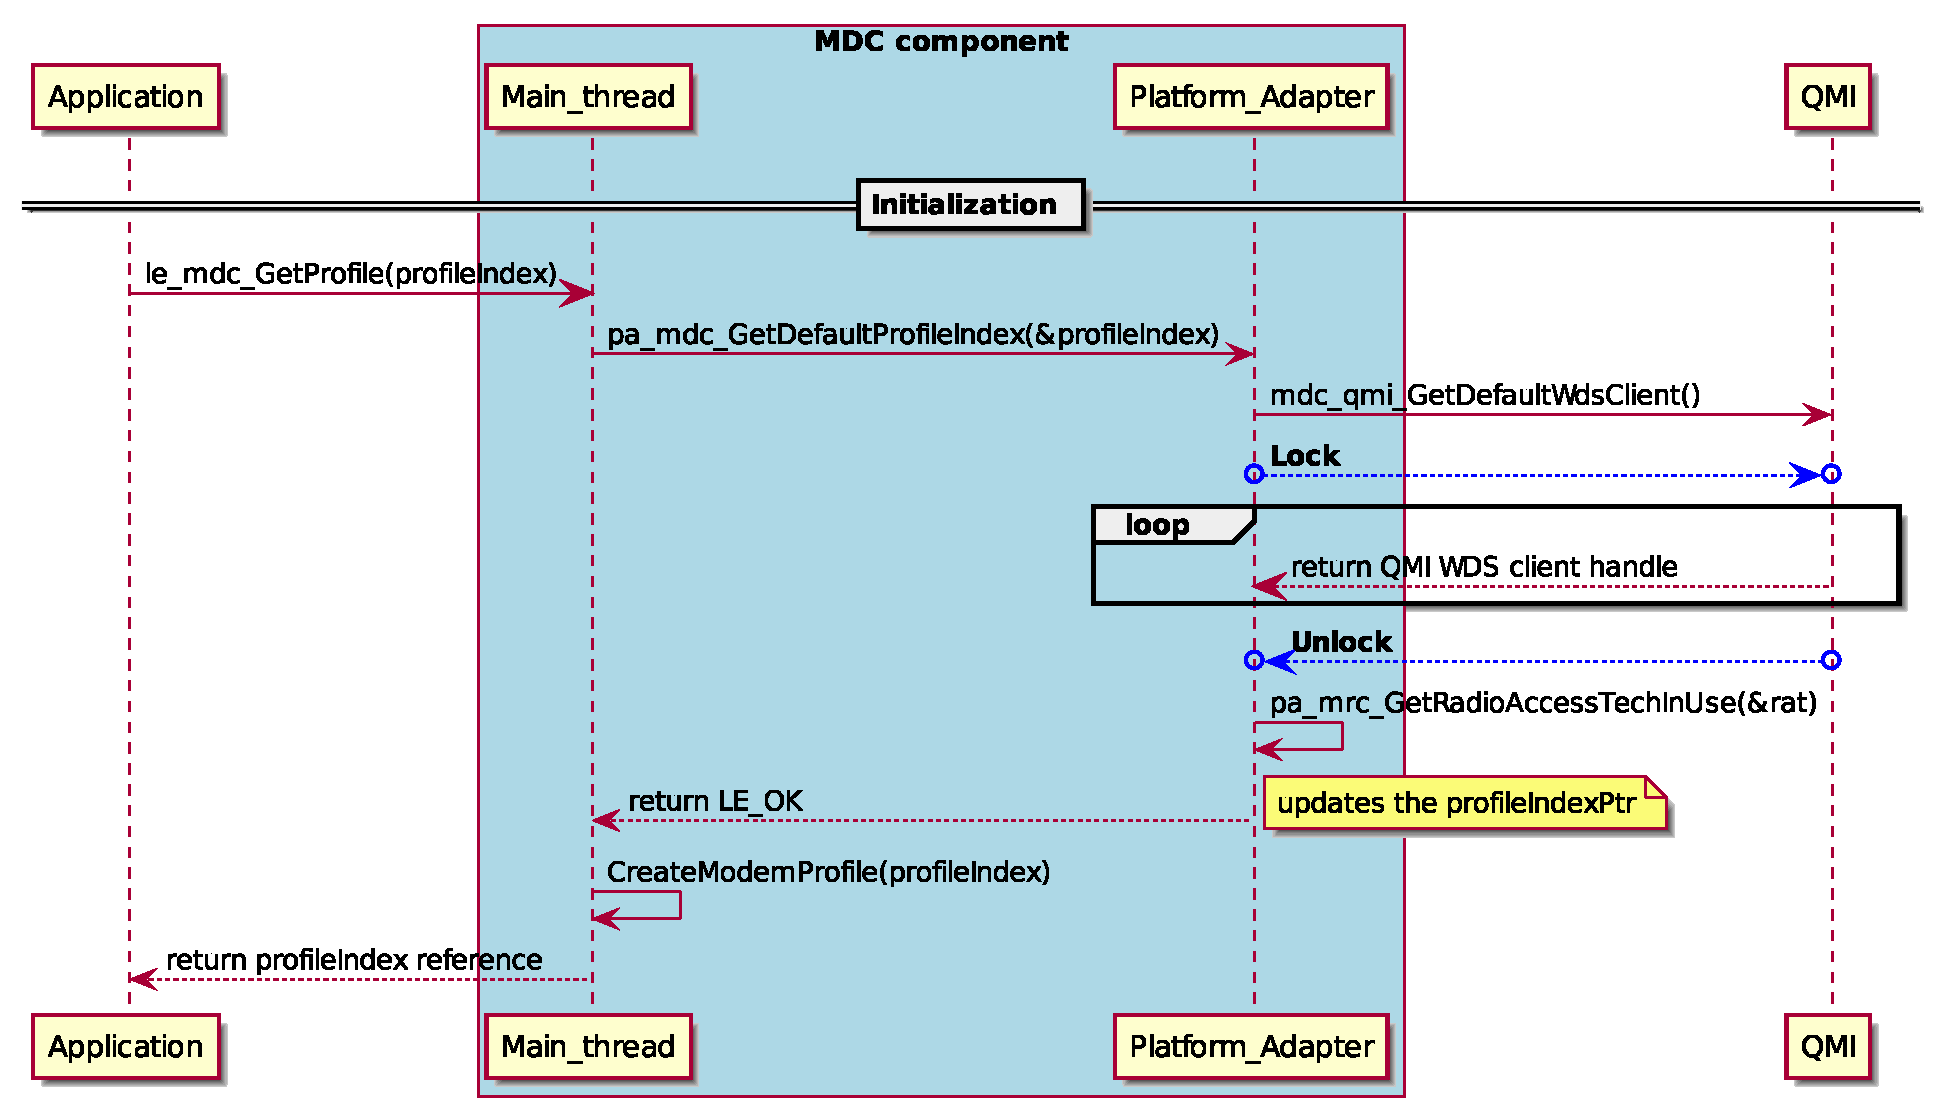
\includegraphics[width=\textwidth,height=\textheight/2,keepaspectratio=true]{le_mdc_GetProfile}}
\end{DoxyImageNoCaption}


The following flow diagram describes the M\+DC start session\+:


\begin{DoxyImageNoCaption}
  \mbox{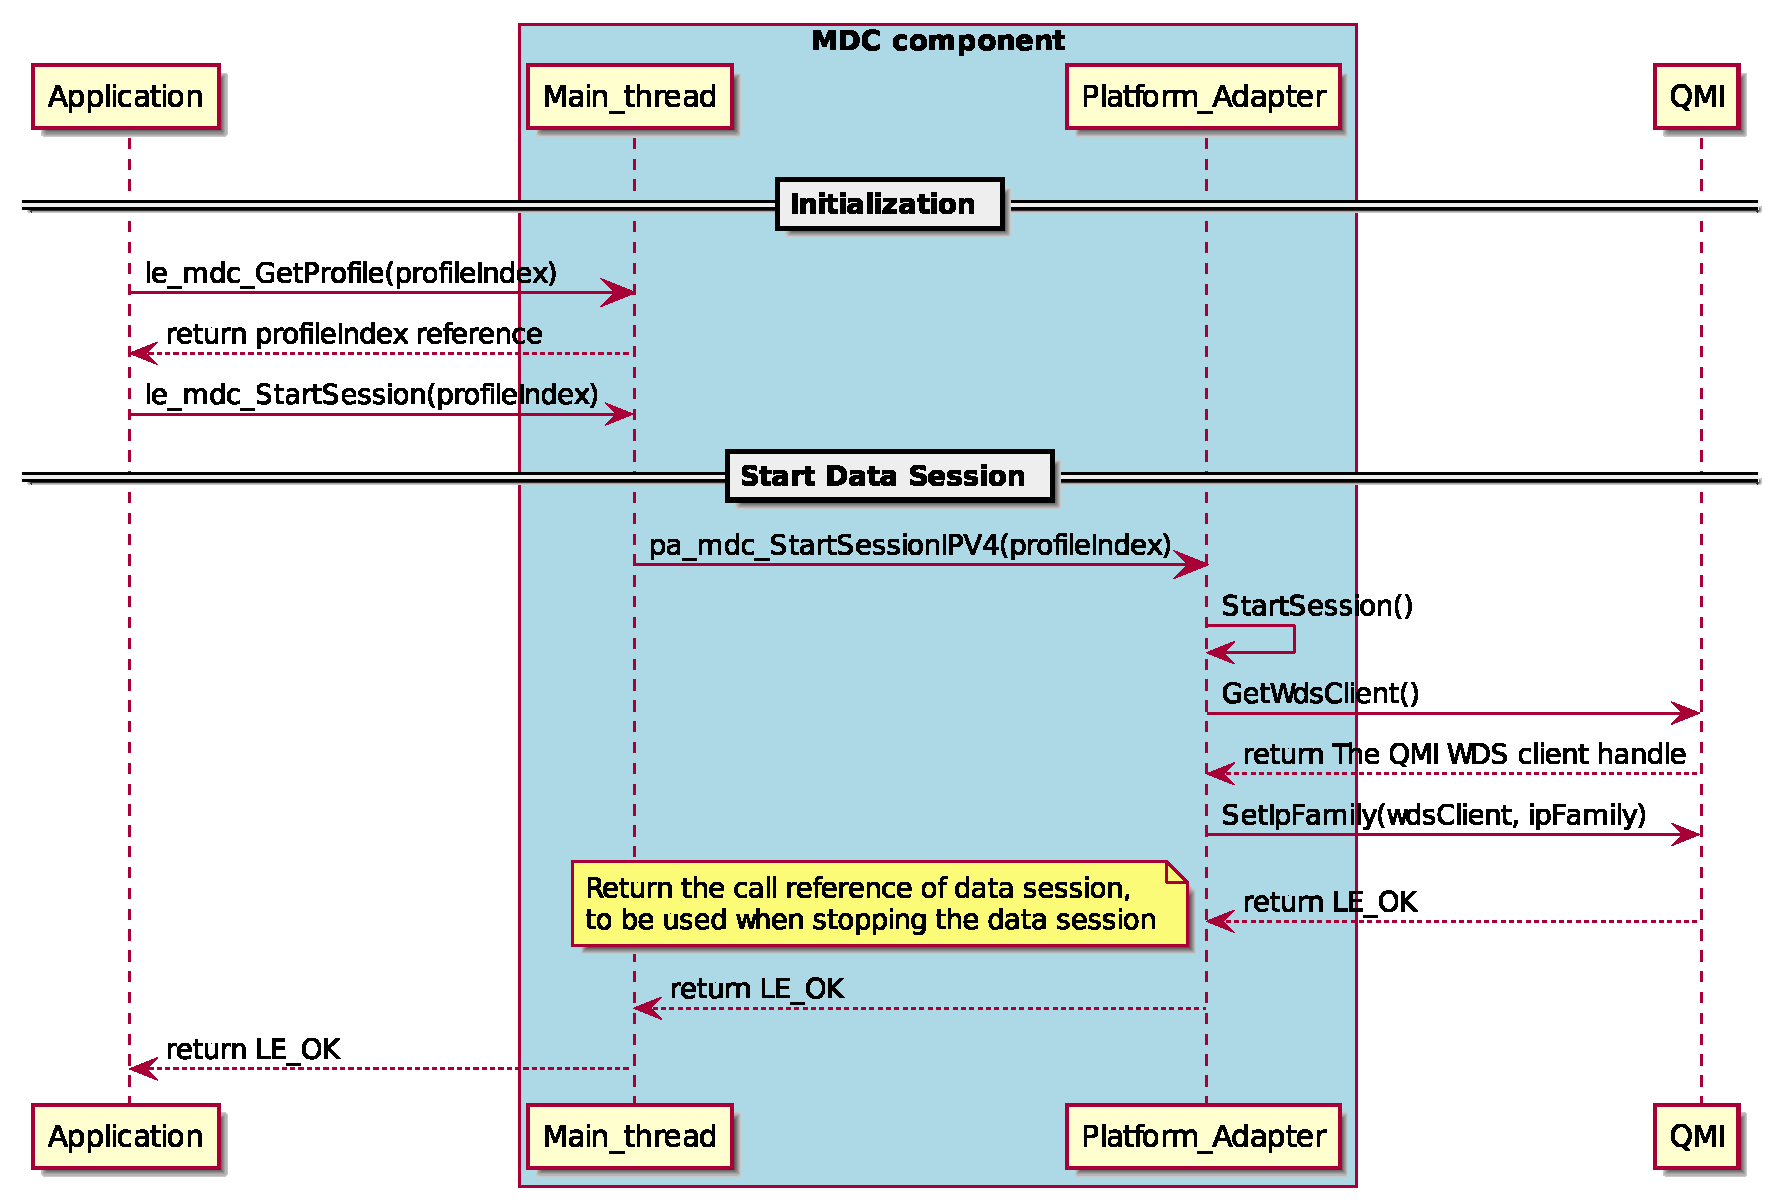
\includegraphics[width=\textwidth,height=\textheight/2,keepaspectratio=true]{le_mdc_StartSession}}
\end{DoxyImageNoCaption}


The following flow diagram describes the M\+DC stop session\+:


\begin{DoxyImageNoCaption}
  \mbox{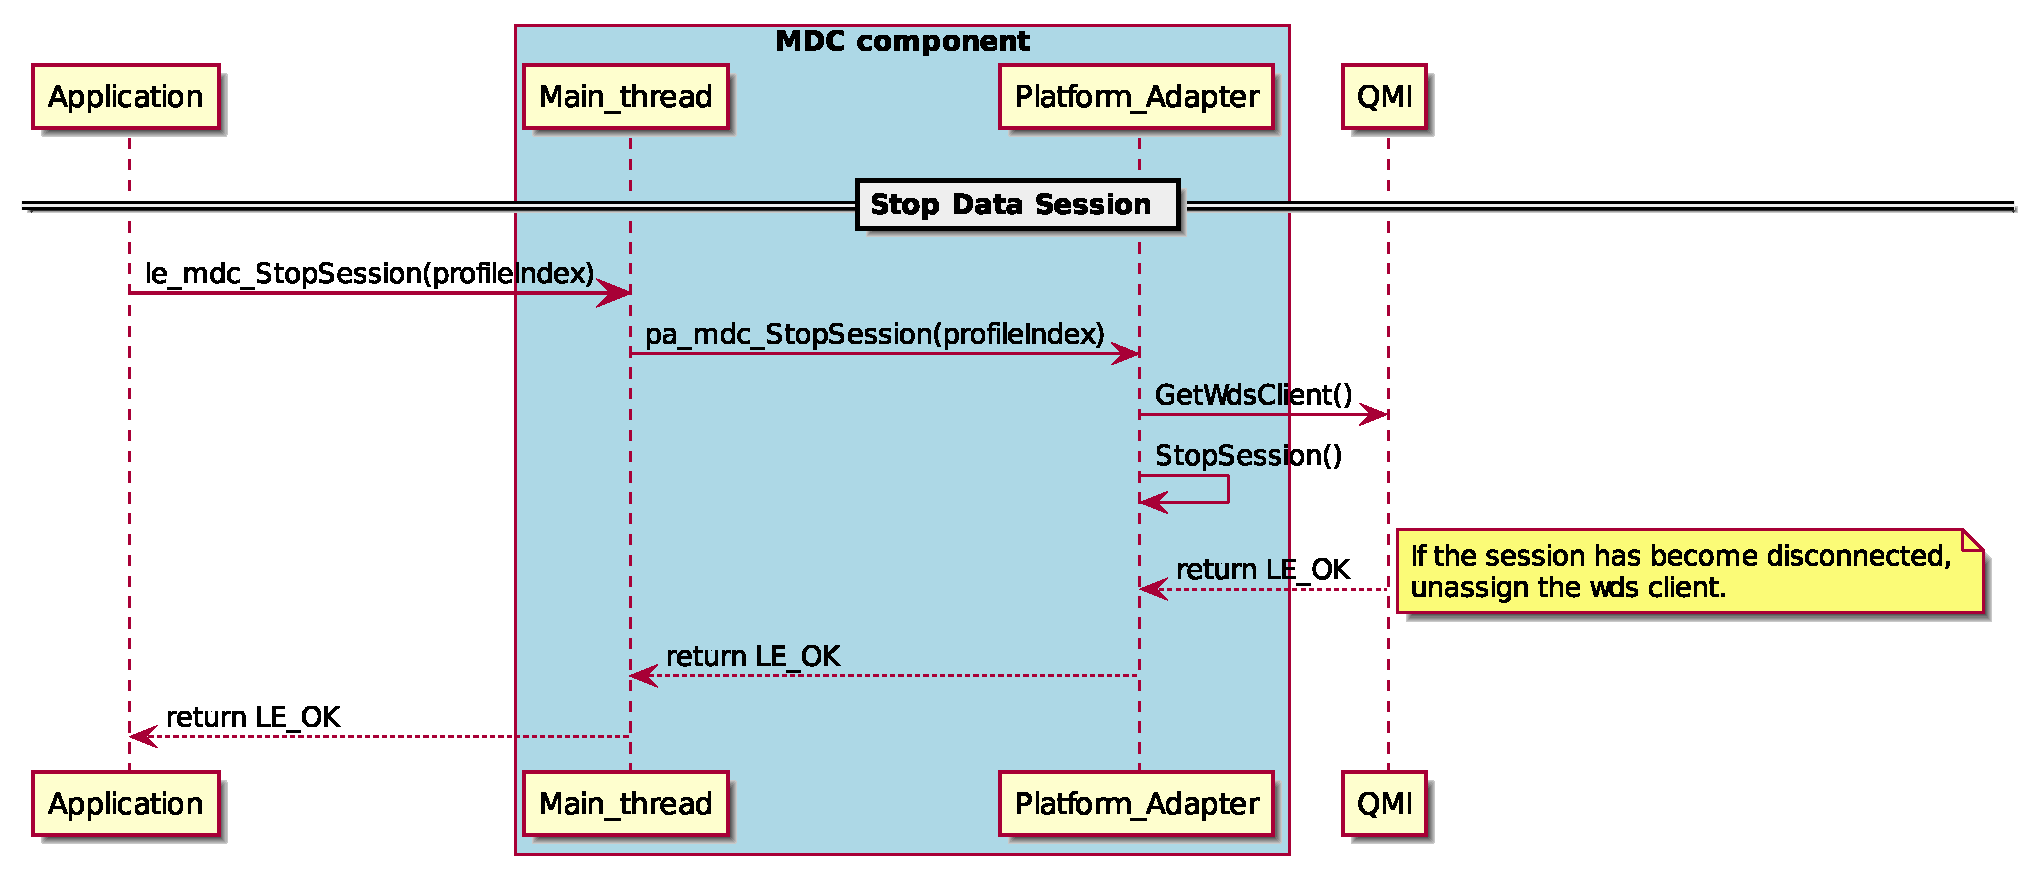
\includegraphics[width=\textwidth,height=\textheight/2,keepaspectratio=true]{le_mdc_StopSession}}
\end{DoxyImageNoCaption}


Copyright (C) Sierra Wireless Inc. \hypertarget{c_SDD_eCall}{}\section{e\+Call S\+DD}\label{c_SDD_eCall}
\hypertarget{c_SDD_eCall_eCall}{}\subsection{e\+Call}\label{c_SDD_eCall_eCall}
\hypertarget{c_SDD_mdc_Overview}{}\subsubsection{Overview}\label{c_SDD_mdc_Overview}
Ecall is a technology initiative intended to bring rapid assistance to auto accidents. When a serious vehicle accident occurs, sensors automatically trigger an e\+Call. When activated, the in-\/vehicle system (I\+VS) establishes a 112-\/voice connection. At the same time, a digital \char`\"{}minimum set of data\char`\"{} (M\+SD) message is sent over the voice call using in-\/band modem signals. The M\+SD includes accident information like time, location, driving direction and vehicle description.\hypertarget{c_SDD_eCall_le_ecall_operation}{}\subsubsection{Operation modes}\label{c_SDD_eCall_le_ecall_operation}
The L\+E\+\_\+\+E\+C\+A\+LL component offers interfaces for the Client Application to handle the different e\+Call operation modes. In e\+Call Only mode, the I\+VS does not register to the network beforehand, thus not giving any burden to the network. It does however listen to cells to be prepared for make an e\+Call. To allow callback after an e\+Call, it is stated that the I\+VS should stay registered on the network for a time interval determined by the N\+AD deregistration time setting. There are number of timers running on the I\+VS side. T9 and T10 are timers tracking these registration times.

The modem can be configured to operate in three different operation modes\+:
\begin{DoxyItemize}
\item \hyperlink{le__ecall__interface_8h_a042d52c84b5b679ab32dd814c5b0be9e}{le\+\_\+ecall\+\_\+\+Force\+Only\+Mode()}\+: this function configures the e\+Call operation mode to e\+Call only. At startup, the modem doesn\textquotesingle{}t try to register on the Cellular network. This function forces the modem to behave as e\+Call only mode whatever U/\+S\+IM operation mode. The change doesn\textquotesingle{}t persist over power cycles. This function can be called before making an e\+Call.
\item \hyperlink{le__ecall__interface_8h_ad468828b0024de378d91ea9c30fd6f3f}{le\+\_\+ecall\+\_\+\+Force\+Persistent\+Only\+Mode()}\+: Same as \hyperlink{le__ecall__interface_8h_a042d52c84b5b679ab32dd814c5b0be9e}{le\+\_\+ecall\+\_\+\+Force\+Only\+Mode()}, but the change persists over power cycles.
\item \hyperlink{le__ecall__interface_8h_a924114fa7fab10c3f351766a76134f34}{le\+\_\+ecall\+\_\+\+Exit\+Only\+Mode()}\+: this function exits from e\+Call Only mode. It configures the e\+Call operation mode to Normal mode, the modem uses the default operation mode at power up (or after U/\+S\+IM hotswap). The modem behaves following the U/\+S\+IM e\+Call operation mode; for example the U/\+S\+IM can be configured only for e\+Call, or a combination of e\+Call and commercial service provision.
\item \hyperlink{le__ecall__interface_8h_a8e245065491b14f46405e415ea17b6b8}{le\+\_\+ecall\+\_\+\+Get\+Configured\+Operation\+Mode()}\+: this function allows the user to retrieve the configured Operation mode.
\end{DoxyItemize}

The configured operation mode can be\+:
\begin{DoxyItemize}
\item {\ttfamily L\+E\+\_\+\+E\+C\+A\+L\+L\+\_\+\+N\+O\+R\+M\+A\+L\+\_\+\+M\+O\+DE} \+: normal mode. The modem behaves following the U/\+S\+IM e\+Call operation mode; for example the U/\+S\+IM can be configured only for e\+Call, or a combination of e\+Call and commercial service provision.
\item {\ttfamily L\+E\+\_\+\+E\+C\+A\+L\+L\+\_\+\+O\+N\+L\+Y\+\_\+\+M\+O\+DE} \+: e\+Call only mode. This mode is enabled following the U/\+S\+IM operation mode if U/\+S\+IM is e\+Call only sim or forced by application through the \hyperlink{le__ecall__interface_8h_a042d52c84b5b679ab32dd814c5b0be9e}{le\+\_\+ecall\+\_\+\+Force\+Only\+Mode()} function.
\item {\ttfamily L\+E\+\_\+\+E\+C\+A\+L\+L\+\_\+\+F\+O\+R\+C\+E\+D\+\_\+\+P\+E\+R\+S\+I\+S\+T\+E\+N\+T\+\_\+\+O\+N\+L\+Y\+\_\+\+M\+O\+DE} \+: persistent e\+Call only mode.
\end{DoxyItemize}


\begin{DoxyCodeInclude}
    \hyperlink{le__log_8h_ac0dbbef91dc0fed449d0092ff0557b39}{LE\_ASSERT}((res=\hyperlink{le__ecall__interface_8h_a042d52c84b5b679ab32dd814c5b0be9e}{le\_ecall\_ForceOnlyMode}()) == LE\_OK);
    \hyperlink{le__log_8h_ac0dbbef91dc0fed449d0092ff0557b39}{LE\_ASSERT}((res=\hyperlink{le__ecall__interface_8h_a8e245065491b14f46405e415ea17b6b8}{le\_ecall\_GetConfiguredOperationMode}(&mode)) 
      == LE\_OK);
    \hyperlink{le__log_8h_ac0dbbef91dc0fed449d0092ff0557b39}{LE\_ASSERT}(mode == \hyperlink{le__ecall__interface_8h_af762f89b222e4cc18e9646c6e4b945b9a841847f485e780277e11d1e942d8800d}{LE\_ECALL\_ONLY\_MODE});

    \hyperlink{le__log_8h_ac0dbbef91dc0fed449d0092ff0557b39}{LE\_ASSERT}((res=\hyperlink{le__ecall__interface_8h_ad468828b0024de378d91ea9c30fd6f3f}{le\_ecall\_ForcePersistentOnlyMode}()) == LE\_OK);
    \hyperlink{le__log_8h_ac0dbbef91dc0fed449d0092ff0557b39}{LE\_ASSERT}((res=\hyperlink{le__ecall__interface_8h_a8e245065491b14f46405e415ea17b6b8}{le\_ecall\_GetConfiguredOperationMode}(&mode)) 
      == LE\_OK);
    \hyperlink{le__log_8h_ac0dbbef91dc0fed449d0092ff0557b39}{LE\_ASSERT}(mode == \hyperlink{le__ecall__interface_8h_af762f89b222e4cc18e9646c6e4b945b9a6d328d963d60c73e04af260f8dae7257}{LE\_ECALL\_FORCED\_PERSISTENT\_ONLY\_MODE});

    \hyperlink{le__log_8h_ac0dbbef91dc0fed449d0092ff0557b39}{LE\_ASSERT}((res=\hyperlink{le__ecall__interface_8h_a924114fa7fab10c3f351766a76134f34}{le\_ecall\_ExitOnlyMode}()) == LE\_OK);
    \hyperlink{le__log_8h_ac0dbbef91dc0fed449d0092ff0557b39}{LE\_ASSERT}((res=\hyperlink{le__ecall__interface_8h_a8e245065491b14f46405e415ea17b6b8}{le\_ecall\_GetConfiguredOperationMode}(&mode)) 
      == LE\_OK);
    \hyperlink{le__log_8h_ac0dbbef91dc0fed449d0092ff0557b39}{LE\_ASSERT}(mode == \hyperlink{le__ecall__interface_8h_af762f89b222e4cc18e9646c6e4b945b9a9d8e54c64e4796257880e146b15521f5}{LE\_ECALL\_NORMAL\_MODE});
\end{DoxyCodeInclude}
 \hypertarget{c_SDD_eCall_le_ecall_session}{}\subsubsection{e\+Call Session}\label{c_SDD_eCall_le_ecall_session}
An e\+Call session is started by creating an e\+Call object with the \hyperlink{le__ecall__interface_8h_aad7fa3b34d9d72a2f1d4baa681ba25cc}{le\+\_\+ecall\+\_\+\+Create()} function. The e\+Call session can then be stopped with \hyperlink{le__ecall__interface_8h_a85800c86f9709fb7baa7219cc762181c}{le\+\_\+ecall\+\_\+\+End()}.

The e\+Call type and the kind of activation are specified using different functions to start the e\+Call session\+:
\begin{DoxyItemize}
\item \hyperlink{le__ecall__interface_8h_ab106c3ca87fc8dd8239d2849df932122}{le\+\_\+ecall\+\_\+\+Start\+Manual()}\+: initiate a manual e\+Call session (triggered by a passenger)
\item \hyperlink{le__ecall__interface_8h_aa25256eeacefcf00c14763ef294c7667}{le\+\_\+ecall\+\_\+\+Start\+Automatic()}\+: initiate an automatic e\+Call session (automatically triggered by the I\+VS in case of accident)
\item \hyperlink{le__ecall__interface_8h_aa5d23a1bea370b1ae29fc52d7a89d947}{le\+\_\+ecall\+\_\+\+Start\+Test()}\+: initiate a test e\+Call session (to test the communication between the I\+VS and the P\+S\+AP (Public Safety Answering Point, emergency operator))
\end{DoxyItemize}

When the e\+Call object is no longer needed, call \hyperlink{le__ecall__interface_8h_af1221deb68c46912748f65505b3e4919}{le\+\_\+ecall\+\_\+\+Delete()} to free all allocated resources associated with the object.

The current state of an e\+Call session can be queried using \hyperlink{le__ecall__interface_8h_a7881e794b9249222edde10f76d7663c9}{le\+\_\+ecall\+\_\+\+Get\+State()}. Alternatively, an application can register a handler be notified when the session state changes. The handler can be managed using \hyperlink{le__ecall__interface_8h_a453b64579f2884f1d26981bca38a201c}{le\+\_\+ecall\+\_\+\+Add\+State\+Change\+Handler()} and \hyperlink{le__ecall__interface_8h_aa2eb6eb76611d78e27b71426b2160cb1}{le\+\_\+ecall\+\_\+\+Remove\+State\+Change\+Handler()}.

An application can also call \hyperlink{le__ecall__interface_8h_a771b2ef399a8fbf3b80c4eb11152c06a}{le\+\_\+ecall\+\_\+\+Get\+Termination\+Reason()} to retrieve the reason of the call termination when call state is L\+E\+\_\+\+E\+C\+A\+L\+L\+\_\+\+S\+T\+A\+T\+E\+\_\+\+D\+I\+S\+C\+O\+N\+N\+E\+C\+T\+ED and \hyperlink{le__ecall__interface_8h_a8ffb7fb207537ea4574823285ebb6ca1}{le\+\_\+ecall\+\_\+\+Get\+Platform\+Specific\+Termination\+Code()} to get platform specific termination code.


\begin{DoxyCodeInclude}
    \hyperlink{le__log_8h_ac0dbbef91dc0fed449d0092ff0557b39}{LE\_ASSERT}((testECallRef=\hyperlink{le__ecall__interface_8h_aad7fa3b34d9d72a2f1d4baa681ba25cc}{le\_ecall\_Create}()) != NULL);

    \hyperlink{le__log_8h_ac0dbbef91dc0fed449d0092ff0557b39}{LE\_ASSERT}(\hyperlink{le__ecall__interface_8h_a7d8d8c1e1f49af2f6145836975d20aeb}{le\_ecall\_ImportMsd}(testECallRef, ImportedMsd, \textcolor{keyword}{sizeof}(ImportedMsd))
       == LE\_OK);

    \hyperlink{le__log_8h_ac0dbbef91dc0fed449d0092ff0557b39}{LE\_ASSERT}(\hyperlink{le__ecall__interface_8h_ab106c3ca87fc8dd8239d2849df932122}{le\_ecall\_StartManual}(testECallRef) == LE\_OK);

    \hyperlink{le__log_8h_ac0dbbef91dc0fed449d0092ff0557b39}{LE\_ASSERT}(\hyperlink{le__ecall__interface_8h_aa5d23a1bea370b1ae29fc52d7a89d947}{le\_ecall\_StartTest}(testECallRef) == 
      \hyperlink{le__basics_8h_a1cca095ed6ebab24b57a636382a6c86ca92b0367090993d8b41d1560663d01e8d}{LE\_BUSY});
    \hyperlink{le__log_8h_ac0dbbef91dc0fed449d0092ff0557b39}{LE\_ASSERT}(\hyperlink{le__ecall__interface_8h_aa25256eeacefcf00c14763ef294c7667}{le\_ecall\_StartAutomatic}(testECallRef) == 
      \hyperlink{le__basics_8h_a1cca095ed6ebab24b57a636382a6c86ca92b0367090993d8b41d1560663d01e8d}{LE\_BUSY});

    \hyperlink{le__log_8h_ac0dbbef91dc0fed449d0092ff0557b39}{LE\_ASSERT}(\hyperlink{le__ecall__interface_8h_a85800c86f9709fb7baa7219cc762181c}{le\_ecall\_End}(testECallRef) == LE\_OK);

    state=\hyperlink{le__ecall__interface_8h_a7881e794b9249222edde10f76d7663c9}{le\_ecall\_GetState}(testECallRef);
    \hyperlink{le__log_8h_ac0dbbef91dc0fed449d0092ff0557b39}{LE\_ASSERT}(((state>=\hyperlink{le__ecall__interface_8h_a233609e4724e549a1405f9177c0a07dda94ba7aacca9dfe74c4733515a7ba2c5e}{LE\_ECALL\_STATE\_STARTED}) && (state<=
      \hyperlink{le__ecall__interface_8h_a233609e4724e549a1405f9177c0a07dda5275385371c51e441a9eb97626c271b4}{LE\_ECALL\_STATE\_FAILED})));

    \hyperlink{le__ecall__interface_8h_af1221deb68c46912748f65505b3e4919}{le\_ecall\_Delete}(testECallRef);
\end{DoxyCodeInclude}
 \hypertarget{c_SDD_eCall_le_ecall_msd}{}\subsubsection{Minimum Set of Data (\+M\+S\+D)}\label{c_SDD_eCall_le_ecall_msd}
The dynamic values of the M\+SD can be set with\+:
\begin{DoxyItemize}
\item \hyperlink{le__ecall__interface_8h_a2b56b7b7fd7f936c144d30eba7815908}{le\+\_\+ecall\+\_\+\+Set\+Msd\+Position()} sets the position of the vehicle.
\item \hyperlink{le__ecall__interface_8h_af3cfea09eea1b1ba39648798070ad139}{le\+\_\+ecall\+\_\+\+Set\+Msd\+Position\+N1()} sets the first delta position of the vehicle.
\item \hyperlink{le__ecall__interface_8h_a6b25b9b242ba114f31ae2f853070bf11}{le\+\_\+ecall\+\_\+\+Set\+Msd\+Position\+N2()} sets the second delta position of the vehicle.
\item \hyperlink{le__ecall__interface_8h_a8c009bb03d61dcd0ffbd9e986b692a85}{le\+\_\+ecall\+\_\+\+Set\+Msd\+Passengers\+Count()} sets the number of passengers.
\end{DoxyItemize}

The M\+SD is automatically encoded with the values previously set with le\+\_\+ecall\+\_\+\+Set\+Msd\+Xxx() A\+P\+Is.

\begin{DoxyWarning}{Warning}
Those functions return a L\+E\+\_\+\+D\+U\+P\+L\+I\+C\+A\+TE error when the M\+SD has been already imported with \hyperlink{le__ecall__interface_8h_a7d8d8c1e1f49af2f6145836975d20aeb}{le\+\_\+ecall\+\_\+\+Import\+Msd()} function.
\end{DoxyWarning}

\begin{DoxyCodeInclude}
    \hyperlink{le__log_8h_ac0dbbef91dc0fed449d0092ff0557b39}{LE\_ASSERT}(\hyperlink{le__ecall__interface_8h_a2b56b7b7fd7f936c144d30eba7815908}{le\_ecall\_SetMsdPosition}(testECallRef, \textcolor{keyword}{true}, +48898064, +22180
      92, 0) == LE\_OK);
    \hyperlink{le__log_8h_ac0dbbef91dc0fed449d0092ff0557b39}{LE\_ASSERT}(\hyperlink{le__ecall__interface_8h_af3cfea09eea1b1ba39648798070ad139}{le\_ecall\_SetMsdPositionN1}(testECallRef,511,511) == LE\_OK);
    \hyperlink{le__log_8h_ac0dbbef91dc0fed449d0092ff0557b39}{LE\_ASSERT}(\hyperlink{le__ecall__interface_8h_a6b25b9b242ba114f31ae2f853070bf11}{le\_ecall\_SetMsdPositionN2}(testECallRef,-512,-512) == LE\_OK)
      ;

    \hyperlink{le__log_8h_ac0dbbef91dc0fed449d0092ff0557b39}{LE\_ASSERT}(\hyperlink{le__ecall__interface_8h_a8c009bb03d61dcd0ffbd9e986b692a85}{le\_ecall\_SetMsdPassengersCount}(testECallRef, 3) == 
      LE\_OK);
\textcolor{comment}{}
\textcolor{comment}{    //! [ExportMsd]}
\textcolor{comment}{}    \hyperlink{le__log_8h_a7cd2daa3d4af1de4d29e0eed95187484}{LE\_ASSERT\_OK}(\hyperlink{le__ecall__interface_8h_adc9610dae7a6ba87c064f8dd271a57b4}{le\_ecall\_ExportMsd}(testECallRef, exportMsd, &msdSize));

    \textcolor{comment}{// Check LE\_DUPLICATE on le\_ecall\_SetMsdPosition and le\_ecall\_SetMsdPassengersCount}
    \hyperlink{le__log_8h_ac0dbbef91dc0fed449d0092ff0557b39}{LE\_ASSERT}(\hyperlink{le__ecall__interface_8h_a7d8d8c1e1f49af2f6145836975d20aeb}{le\_ecall\_ImportMsd}(testECallRef, ImportedMsd, \textcolor{keyword}{sizeof}(ImportedMsd))
       == LE\_OK);

    \hyperlink{le__log_8h_ac0dbbef91dc0fed449d0092ff0557b39}{LE\_ASSERT}(\hyperlink{le__ecall__interface_8h_adc9610dae7a6ba87c064f8dd271a57b4}{le\_ecall\_ExportMsd}(testECallRef, exportMsd, &msdSize) == 
      \hyperlink{le__basics_8h_a1cca095ed6ebab24b57a636382a6c86cac26034778a666ee720b110c2fb1647ea}{LE\_DUPLICATE});\textcolor{comment}{}
\textcolor{comment}{    //! [ExportMsd]}
\textcolor{comment}{}
    \hyperlink{le__log_8h_ac0dbbef91dc0fed449d0092ff0557b39}{LE\_ASSERT}(\hyperlink{le__ecall__interface_8h_a2b56b7b7fd7f936c144d30eba7815908}{le\_ecall\_SetMsdPosition}(testECallRef, \textcolor{keyword}{true}, +48070380, -11310
      000, 45) ==
                                                                                
      \hyperlink{le__basics_8h_a1cca095ed6ebab24b57a636382a6c86cac26034778a666ee720b110c2fb1647ea}{LE\_DUPLICATE});
    \hyperlink{le__log_8h_ac0dbbef91dc0fed449d0092ff0557b39}{LE\_ASSERT}(\hyperlink{le__ecall__interface_8h_af3cfea09eea1b1ba39648798070ad139}{le\_ecall\_SetMsdPositionN1}(testECallRef, 511, 511) == 
      \hyperlink{le__basics_8h_a1cca095ed6ebab24b57a636382a6c86cac26034778a666ee720b110c2fb1647ea}{LE\_DUPLICATE});
    \hyperlink{le__log_8h_ac0dbbef91dc0fed449d0092ff0557b39}{LE\_ASSERT}(\hyperlink{le__ecall__interface_8h_a6b25b9b242ba114f31ae2f853070bf11}{le\_ecall\_SetMsdPositionN2}(testECallRef, -512, -512) == 
      \hyperlink{le__basics_8h_a1cca095ed6ebab24b57a636382a6c86cac26034778a666ee720b110c2fb1647ea}{LE\_DUPLICATE});
    \hyperlink{le__log_8h_ac0dbbef91dc0fed449d0092ff0557b39}{LE\_ASSERT}(\hyperlink{le__ecall__interface_8h_a8c009bb03d61dcd0ffbd9e986b692a85}{le\_ecall\_SetMsdPassengersCount}(testECallRef, 3) == 
      \hyperlink{le__basics_8h_a1cca095ed6ebab24b57a636382a6c86cac26034778a666ee720b110c2fb1647ea}{LE\_DUPLICATE});
\end{DoxyCodeInclude}
 The M\+SD transmission mode can be set or get with\+:
\begin{DoxyItemize}
\item \hyperlink{le__ecall__interface_8h_a00d3dbc99884375cf2487d6640767c40}{le\+\_\+ecall\+\_\+\+Set\+Msd\+Tx\+Mode()}
\item \hyperlink{le__ecall__interface_8h_a4319df67dc451fecb72e4e60ba7b6f6e}{le\+\_\+ecall\+\_\+\+Get\+Msd\+Tx\+Mode()}
\end{DoxyItemize}

The transmission mode can be\+:
\begin{DoxyItemize}
\item {\ttfamily L\+E\+\_\+\+E\+C\+A\+L\+L\+\_\+\+T\+X\+\_\+\+M\+O\+D\+E\+\_\+\+P\+U\+SH} \+: the M\+SD is pushed by the I\+VS
\item {\ttfamily L\+E\+\_\+\+E\+C\+A\+L\+L\+\_\+\+T\+X\+\_\+\+M\+O\+D\+E\+\_\+\+P\+U\+LL} \+: the M\+SD is sent when requested by the P\+S\+AP
\end{DoxyItemize}

Legato sets the correct transmission mode during e\+Call start and redialing based on e\+Call standard. There is no need to call these A\+P\+Is explicitly.


\begin{DoxyCodeInclude}
    \hyperlink{le__log_8h_ac0dbbef91dc0fed449d0092ff0557b39}{LE\_ASSERT}(\hyperlink{le__ecall__interface_8h_a00d3dbc99884375cf2487d6640767c40}{le\_ecall\_SetMsdTxMode}(
      \hyperlink{le__ecall__interface_8h_adbaa600a7ab66371afddb909b1a113bdafe1cddc2df801a67c7f02020c0dd1127}{LE\_ECALL\_TX\_MODE\_PUSH}) == LE\_OK);
    \hyperlink{le__log_8h_ac0dbbef91dc0fed449d0092ff0557b39}{LE\_ASSERT}(\hyperlink{le__ecall__interface_8h_a4319df67dc451fecb72e4e60ba7b6f6e}{le\_ecall\_GetMsdTxMode}(&mode) == LE\_OK);
\end{DoxyCodeInclude}
 It\textquotesingle{}s possible to import a prepared M\+SD using the \hyperlink{le__ecall__interface_8h_a7d8d8c1e1f49af2f6145836975d20aeb}{le\+\_\+ecall\+\_\+\+Import\+Msd()} function. The prepared M\+SD must answer the requirements described in the \char`\"{}\+E\+N 15722\+:2013\char`\"{} publication (this publication has been prepared by Technical Committee C\+E\+N/\+TC 278 “\+Intelligent Transport Systems").

\begin{DoxyWarning}{Warning}
The imported M\+SD doesn\textquotesingle{}t take into account the values provided by the le\+\_\+ecall\+\_\+\+Set\+Msd\+Xxx() functions. It overwrites any previous imported M\+SD or encoded M\+SD.

The imported M\+SD overwrites the control flags (automatic\+Activation and test\+Call) set by le\+\_\+ecall\+\_\+\+Start\+Xxx() functions (Manual, Automatic, Test). The User App is in charge of their correct settings.
\end{DoxyWarning}
The encoded M\+SD can be retrieved with \hyperlink{le__ecall__interface_8h_adc9610dae7a6ba87c064f8dd271a57b4}{le\+\_\+ecall\+\_\+\+Export\+Msd()} function. It also exports the optional additional data of E\+R\+A-\/\+Glonass. \hyperlink{le__ecall__interface_8h_adc9610dae7a6ba87c064f8dd271a57b4}{le\+\_\+ecall\+\_\+\+Export\+Msd()} A\+PI returns L\+E\+\_\+\+D\+U\+P\+L\+I\+C\+A\+TE if M\+SD is already imported using \hyperlink{le__ecall__interface_8h_a7d8d8c1e1f49af2f6145836975d20aeb}{le\+\_\+ecall\+\_\+\+Import\+Msd()} function.


\begin{DoxyCodeInclude}
    \hyperlink{le__log_8h_a7cd2daa3d4af1de4d29e0eed95187484}{LE\_ASSERT\_OK}(\hyperlink{le__ecall__interface_8h_adc9610dae7a6ba87c064f8dd271a57b4}{le\_ecall\_ExportMsd}(testECallRef, exportMsd, &msdSize));

    \textcolor{comment}{// Check LE\_DUPLICATE on le\_ecall\_SetMsdPosition and le\_ecall\_SetMsdPassengersCount}
    \hyperlink{le__log_8h_ac0dbbef91dc0fed449d0092ff0557b39}{LE\_ASSERT}(\hyperlink{le__ecall__interface_8h_a7d8d8c1e1f49af2f6145836975d20aeb}{le\_ecall\_ImportMsd}(testECallRef, ImportedMsd, \textcolor{keyword}{sizeof}(ImportedMsd))
       == LE\_OK);

    \hyperlink{le__log_8h_ac0dbbef91dc0fed449d0092ff0557b39}{LE\_ASSERT}(\hyperlink{le__ecall__interface_8h_adc9610dae7a6ba87c064f8dd271a57b4}{le\_ecall\_ExportMsd}(testECallRef, exportMsd, &msdSize) == 
      \hyperlink{le__basics_8h_a1cca095ed6ebab24b57a636382a6c86cac26034778a666ee720b110c2fb1647ea}{LE\_DUPLICATE});
\end{DoxyCodeInclude}
 \begin{DoxyNote}{Note}
The User app must perform the M\+SD transmission by calling \hyperlink{le__ecall__interface_8h_a344e4c29208e576e81dda113f786529e}{le\+\_\+ecall\+\_\+\+Send\+Msd()} when the L\+E\+\_\+\+E\+C\+A\+L\+L\+\_\+\+S\+T\+A\+T\+E\+\_\+\+P\+S\+A\+P\+\_\+\+S\+T\+A\+R\+T\+\_\+\+I\+N\+D\+\_\+\+R\+E\+C\+E\+I\+V\+ED event is received. The M\+SD can be updated before calling \hyperlink{le__ecall__interface_8h_a344e4c29208e576e81dda113f786529e}{le\+\_\+ecall\+\_\+\+Send\+Msd()}, using the e\+\_\+ecall\+\_\+\+Import\+Msd() function or the le\+\_\+ecall\+\_\+\+Set\+Msd\+Xxx() functions.
\end{DoxyNote}
Following diagram shows the e\+Call service state machine\+:


\begin{DoxyImageNoCaption}
  \mbox{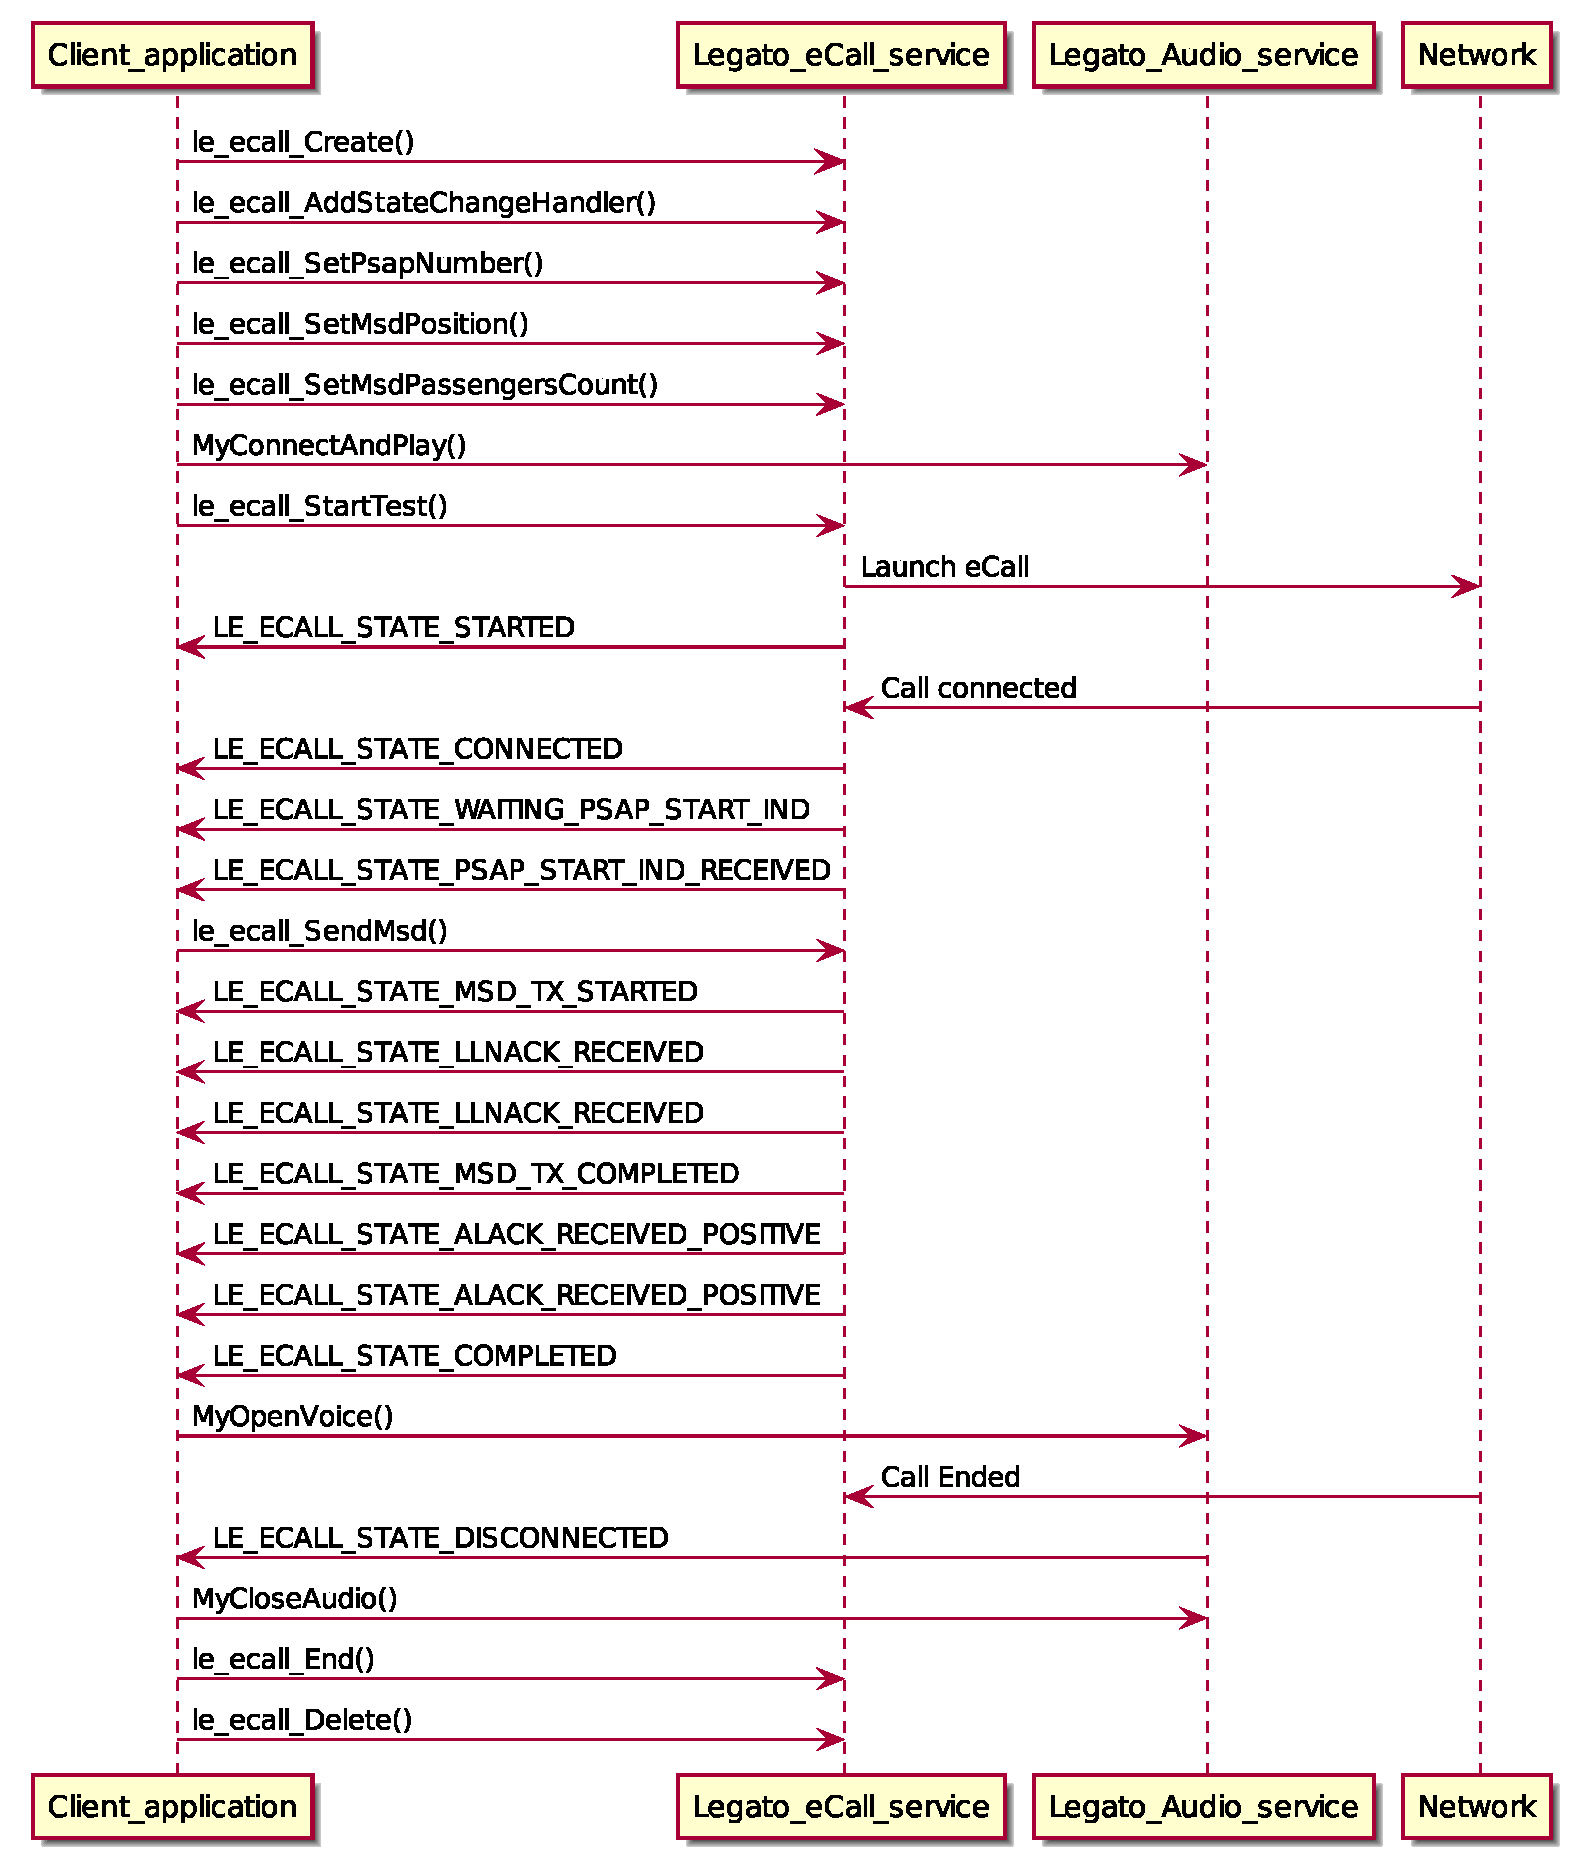
\includegraphics[width=\textwidth,height=\textheight/2,keepaspectratio=true]{le_eCall_state_machine}}
\end{DoxyImageNoCaption}
\hypertarget{c_SDD_eCall_le_ecall_eraglonass}{}\subsubsection{E\+R\+A-\/\+G\+L\+O\+N\+A\+S\+S compliancy}\label{c_SDD_eCall_le_ecall_eraglonass}
To perform an emergency call following the E\+R\+A-\/\+G\+L\+O\+N\+A\+SS requirements, the \textquotesingle{}system\+Standard\textquotesingle{} entry of the configuration database must be set to \textquotesingle{}E\+R\+A-\/\+G\+L\+O\+N\+A\+SS\textquotesingle{}.

Moreover, the User can set some specific configuration settings in accordance with the P\+S\+AP configuration\+:


\begin{DoxyItemize}
\item \hyperlink{le__ecall__interface_8h_a15127a7b0500796257795aaf64acd1e2}{le\+\_\+ecall\+\_\+\+Set\+Era\+Glonass\+Manual\+Dial\+Attempts()}\+: set the M\+A\+N\+U\+A\+L\+\_\+\+D\+I\+A\+L\+\_\+\+A\+T\+T\+E\+M\+P\+TS value. If a dial attempt under manual emergency call initiation failed, it should be repeated maximally E\+C\+A\+L\+L\+\_\+\+M\+A\+N\+U\+A\+L\+\_\+\+D\+I\+A\+L\+\_\+\+A\+T\+T\+E\+M\+P\+T\+S-\/1 times within the maximal time limit of E\+C\+A\+L\+L\+\_\+\+D\+I\+A\+L\+\_\+\+D\+U\+R\+A\+T\+I\+ON. The default value is 10. Redial attempts stop once the call has been cleared down correctly, or if counter / timer reached their limits. Available for both manual and test modes.
\item \hyperlink{le__ecall__interface_8h_a836aaf195c0648d41f4a13f8c7ced736}{le\+\_\+ecall\+\_\+\+Set\+Era\+Glonass\+Auto\+Dial\+Attempts()}\+: set the A\+U\+T\+O\+\_\+\+D\+I\+A\+L\+\_\+\+A\+T\+T\+E\+M\+P\+TS value. If a dial attempt under automatic emergency call initiation failed, it should be repeated maximally E\+C\+A\+L\+L\+\_\+\+A\+U\+T\+O\+\_\+\+D\+I\+A\+L\+\_\+\+A\+T\+T\+E\+M\+P\+T\+S-\/1 times within the maximal time limit of E\+C\+A\+L\+L\+\_\+\+D\+I\+A\+L\+\_\+\+D\+U\+R\+A\+T\+I\+ON. The default value is 10. Redial attempts stop once the call has been cleared down correctly, or if counter / timer reached their limits.
\item \hyperlink{le__ecall__interface_8h_a6c934a9e5aad11eb6f009a6bf34fca19}{le\+\_\+ecall\+\_\+\+Set\+Era\+Glonass\+Dial\+Duration()}\+: set the E\+C\+A\+L\+L\+\_\+\+D\+I\+A\+L\+\_\+\+D\+U\+R\+A\+T\+I\+ON time. It is the maximum time the I\+VS have to connect the emergency call to the P\+S\+AP, including all redial attempts. If the call is not connected within this time (or Manual\+Dial\+Attempts/\+Auto\+Dial\+Attempts dial attempts), it will stop.
\end{DoxyItemize}

The following getter functions let you retrieve the configuration settings values\+:


\begin{DoxyItemize}
\item \hyperlink{le__ecall__interface_8h_a579169dbcb91369caa156d2c0e3462c1}{le\+\_\+ecall\+\_\+\+Get\+Era\+Glonass\+Manual\+Dial\+Attempts()}\+: retrieves the M\+A\+N\+U\+A\+L\+\_\+\+D\+I\+A\+L\+\_\+\+A\+T\+T\+E\+M\+P\+TS value.
\item \hyperlink{le__ecall__interface_8h_af8beed56bd3be9bee8a771e05c498ac8}{le\+\_\+ecall\+\_\+\+Get\+Era\+Glonass\+Auto\+Dial\+Attempts()}\+: retrieves the A\+U\+T\+O\+\_\+\+D\+I\+A\+L\+\_\+\+A\+T\+T\+E\+M\+P\+TS value.
\item \hyperlink{le__ecall__interface_8h_afeb92d26dd8a2c092e96b07f3dc0391d}{le\+\_\+ecall\+\_\+\+Get\+Era\+Glonass\+Dial\+Duration()}\+: retrieves the E\+C\+A\+L\+L\+\_\+\+D\+I\+A\+L\+\_\+\+D\+U\+R\+A\+T\+I\+ON time.
\end{DoxyItemize}


\begin{DoxyCodeInclude}
    \hyperlink{le__log_8h_a7cd2daa3d4af1de4d29e0eed95187484}{LE\_ASSERT\_OK}(\hyperlink{le__ecall__interface_8h_a15127a7b0500796257795aaf64acd1e2}{le\_ecall\_SetEraGlonassManualDialAttempts}
      (7));
    \hyperlink{le__log_8h_a7cd2daa3d4af1de4d29e0eed95187484}{LE\_ASSERT\_OK}(\hyperlink{le__ecall__interface_8h_a579169dbcb91369caa156d2c0e3462c1}{le\_ecall\_GetEraGlonassManualDialAttempts}
      (&attempts));
    \hyperlink{le__log_8h_ac0dbbef91dc0fed449d0092ff0557b39}{LE\_ASSERT}(attempts == 7);

    \hyperlink{le__log_8h_a7cd2daa3d4af1de4d29e0eed95187484}{LE\_ASSERT\_OK}(\hyperlink{le__ecall__interface_8h_a836aaf195c0648d41f4a13f8c7ced736}{le\_ecall\_SetEraGlonassAutoDialAttempts}(9
      ));
    \hyperlink{le__log_8h_a7cd2daa3d4af1de4d29e0eed95187484}{LE\_ASSERT\_OK}(\hyperlink{le__ecall__interface_8h_af8beed56bd3be9bee8a771e05c498ac8}{le\_ecall\_GetEraGlonassAutoDialAttempts}(&
      attempts));
    \hyperlink{le__log_8h_ac0dbbef91dc0fed449d0092ff0557b39}{LE\_ASSERT}(attempts == 9);

    \hyperlink{le__log_8h_a7cd2daa3d4af1de4d29e0eed95187484}{LE\_ASSERT\_OK}(\hyperlink{le__ecall__interface_8h_a6c934a9e5aad11eb6f009a6bf34fca19}{le\_ecall\_SetEraGlonassDialDuration}(240));
    \hyperlink{le__log_8h_a7cd2daa3d4af1de4d29e0eed95187484}{LE\_ASSERT\_OK}(\hyperlink{le__ecall__interface_8h_afeb92d26dd8a2c092e96b07f3dc0391d}{le\_ecall\_GetEraGlonassDialDuration}(&duration
      ));
    \hyperlink{le__log_8h_ac0dbbef91dc0fed449d0092ff0557b39}{LE\_ASSERT}(duration == 240);
\end{DoxyCodeInclude}
 \hypertarget{c_SDD_eCall_le_ecall_eraGlonassData}{}\subsection{E\+R\+A-\/\+G\+L\+O\+N\+A\+S\+S M\+S\+D additional data}\label{c_SDD_eCall_le_ecall_eraGlonassData}
E\+R\+A-\/\+G\+L\+O\+N\+A\+SS additional data are optional and provided in the M\+SD message if any. They are located in M\+SD data block number 12 as optional additional data. E\+R\+A-\/\+G\+L\+O\+N\+A\+SS additional data is encoded using the O\+ID version \char`\"{}1.\+4.\+1\char`\"{} for M\+SD version 1 and the O\+ID version \char`\"{}1.\+4.\+2\char`\"{} for M\+SD version 2. This was assigned to E\+R\+A-\/\+G\+L\+O\+N\+A\+SS optional additional data by C\+EN.

E\+R\+A-\/\+G\+L\+O\+N\+A\+SS M\+SD additional data for M\+SD version 1 describes\+:
\begin{DoxyItemize}
\item The crash severity (Accident Severity Index -\/ A\+S\+I15)
\item The diagnostic result
\item The crash information
\end{DoxyItemize}

E\+R\+A-\/\+G\+L\+O\+N\+A\+SS M\+SD additional data for M\+SD version 2 describes\+:
\begin{DoxyItemize}
\item The crash severity (Accident Severity Index -\/ A\+S\+I15)
\item The diagnostic result
\item The crash information
\item The coordinate system type
\end{DoxyItemize}

E\+R\+A-\/\+G\+L\+O\+N\+A\+SS M\+SD additional data can be specified through the following functions\+:
\begin{DoxyItemize}
\item \hyperlink{le__ecall__interface_8h_a577f3dcd16e53c8a14295ec58c6d2b9a}{le\+\_\+ecall\+\_\+\+Set\+Msd\+Era\+Glonass\+Crash\+Severity()}.
\item \hyperlink{le__ecall__interface_8h_addb2874aacaffba2731354c4ac9428bf}{le\+\_\+ecall\+\_\+\+Reset\+Msd\+Era\+Glonass\+Crash\+Severity()}.
\item \hyperlink{le__ecall__interface_8h_a51ad61edf379cfe07f03fbd71b56df9d}{le\+\_\+ecall\+\_\+\+Set\+Msd\+Era\+Glonass\+Diagnostic\+Result()}.
\item \hyperlink{le__ecall__interface_8h_ad3e06b90843a480d68dc99ead29ae8d0}{le\+\_\+ecall\+\_\+\+Reset\+Msd\+Era\+Glonass\+Diagnostic\+Result()}.
\item \hyperlink{le__ecall__interface_8h_a08c613df57d34eb2a1309738bced5d76}{le\+\_\+ecall\+\_\+\+Set\+Msd\+Era\+Glonass\+Crash\+Info()}.
\item \hyperlink{le__ecall__interface_8h_ab883aa41416ada9746acfbb75a0039a8}{le\+\_\+ecall\+\_\+\+Reset\+Msd\+Era\+Glonass\+Crash\+Info()}.
\item \hyperlink{le__ecall__interface_8h_aba15bc78d2e03b5bf8c16ee366fb39b9}{le\+\_\+ecall\+\_\+\+Set\+Msd\+Era\+Glonass\+Coordinate\+System\+Type()}.
\item \hyperlink{le__ecall__interface_8h_a7ca8cd2cfbf76310d1e65d34dfc3b220}{le\+\_\+ecall\+\_\+\+Reset\+Msd\+Era\+Glonass\+Coordinate\+System\+Type()}.
\end{DoxyItemize}


\begin{DoxyCodeInclude}
    \textcolor{comment}{/* Crash Severity configuration */}
    \hyperlink{le__log_8h_a7cd2daa3d4af1de4d29e0eed95187484}{LE\_ASSERT\_OK}(\hyperlink{le__ecall__interface_8h_a577f3dcd16e53c8a14295ec58c6d2b9a}{le\_ecall\_SetMsdEraGlonassCrashSeverity}(
      testECallRef, 0));
    \hyperlink{le__log_8h_a7cd2daa3d4af1de4d29e0eed95187484}{LE\_ASSERT\_OK}(\hyperlink{le__ecall__interface_8h_addb2874aacaffba2731354c4ac9428bf}{le\_ecall\_ResetMsdEraGlonassCrashSeverity}
      (testECallRef));
    \hyperlink{le__log_8h_a7cd2daa3d4af1de4d29e0eed95187484}{LE\_ASSERT\_OK}(\hyperlink{le__ecall__interface_8h_a577f3dcd16e53c8a14295ec58c6d2b9a}{le\_ecall\_SetMsdEraGlonassCrashSeverity}(
      testECallRef, 99));

    \textcolor{comment}{/* DataDiagnosticResult configuration */}
    \hyperlink{le__log_8h_a7cd2daa3d4af1de4d29e0eed95187484}{LE\_ASSERT\_OK}(\hyperlink{le__ecall__interface_8h_a51ad61edf379cfe07f03fbd71b56df9d}{le\_ecall\_SetMsdEraGlonassDiagnosticResult}
      (testECallRef, 0x3FFFFFFFFFF));
    \hyperlink{le__log_8h_a7cd2daa3d4af1de4d29e0eed95187484}{LE\_ASSERT\_OK}(\hyperlink{le__ecall__interface_8h_a51ad61edf379cfe07f03fbd71b56df9d}{le\_ecall\_SetMsdEraGlonassDiagnosticResult}
      (testECallRef, 0));
    \hyperlink{le__log_8h_a7cd2daa3d4af1de4d29e0eed95187484}{LE\_ASSERT\_OK}(\hyperlink{le__ecall__interface_8h_ad3e06b90843a480d68dc99ead29ae8d0}{le\_ecall\_ResetMsdEraGlonassDiagnosticResult}
      (testECallRef));
    \hyperlink{le__log_8h_a7cd2daa3d4af1de4d29e0eed95187484}{LE\_ASSERT\_OK}(\hyperlink{le__ecall__interface_8h_a51ad61edf379cfe07f03fbd71b56df9d}{le\_ecall\_SetMsdEraGlonassDiagnosticResult}
      (testECallRef,
                 \hyperlink{le__ecall__interface_8h_a777e8d6608b5e40f73696904471519cfa3a666c50c2a85411eb7d723a9553144e}{LE\_ECALL\_DIAG\_RESULT\_PRESENT\_MIC\_CONNECTION\_FAILURE}
      ));

    \textcolor{comment}{/* CrashInfo configuration */}
    \hyperlink{le__log_8h_a7cd2daa3d4af1de4d29e0eed95187484}{LE\_ASSERT\_OK}(\hyperlink{le__ecall__interface_8h_a08c613df57d34eb2a1309738bced5d76}{le\_ecall\_SetMsdEraGlonassCrashInfo}(
      testECallRef, 0xFFFF));
    \hyperlink{le__log_8h_a7cd2daa3d4af1de4d29e0eed95187484}{LE\_ASSERT\_OK}(\hyperlink{le__ecall__interface_8h_a08c613df57d34eb2a1309738bced5d76}{le\_ecall\_SetMsdEraGlonassCrashInfo}(
      testECallRef, 0));
    \hyperlink{le__log_8h_a7cd2daa3d4af1de4d29e0eed95187484}{LE\_ASSERT\_OK}(\hyperlink{le__ecall__interface_8h_ab883aa41416ada9746acfbb75a0039a8}{le\_ecall\_ResetMsdEraGlonassCrashInfo}(
      testECallRef));
    \hyperlink{le__log_8h_a7cd2daa3d4af1de4d29e0eed95187484}{LE\_ASSERT\_OK}(\hyperlink{le__ecall__interface_8h_a08c613df57d34eb2a1309738bced5d76}{le\_ecall\_SetMsdEraGlonassCrashInfo}(
      testECallRef,
                 \hyperlink{le__ecall__interface_8h_ae95239490ffd1ee40a9dfcfe02cbd318a7139e97473edb9bca67b01d3d4f6d5c9}{LE\_ECALL\_CRASH\_INFO\_PRESENT\_CRASH\_FRONT\_OR\_SIDE}
       |
                 \hyperlink{le__ecall__interface_8h_ae95239490ffd1ee40a9dfcfe02cbd318a0e26e57771f2628a39f1c88a5ef08f1b}{LE\_ECALL\_CRASH\_INFO\_CRASH\_FRONT\_OR\_SIDE}));

    \textcolor{comment}{/* Coordinate system type configuration */}
    uint32\_t msdVersion = 0;
    \hyperlink{le__log_8h_a7cd2daa3d4af1de4d29e0eed95187484}{LE\_ASSERT\_OK}(\hyperlink{le__ecall__interface_8h_a4875975bc3f3c8fb78b43ae40322eedd}{le\_ecall\_GetMsdVersion}(&msdVersion));

    \textcolor{comment}{/* If MSD version is 2, set following MSD parameters */}
    \textcolor{keywordflow}{if} (2 == msdVersion)
    \{
        \hyperlink{le__log_8h_a7cd2daa3d4af1de4d29e0eed95187484}{LE\_ASSERT\_OK}(\hyperlink{le__ecall__interface_8h_aba15bc78d2e03b5bf8c16ee366fb39b9}{le\_ecall\_SetMsdEraGlonassCoordinateSystemType}
      (testECallRef,
                                                 
      \hyperlink{le__ecall__interface_8h_a598bec665c1563eae7a153662e51f446a34ec7e90e068e0979628414832ce3865}{LE\_ECALL\_MSD\_COORDINATE\_SYSTEM\_TYPE\_PZ90}));
        \hyperlink{le__log_8h_a7cd2daa3d4af1de4d29e0eed95187484}{LE\_ASSERT\_OK}(\hyperlink{le__ecall__interface_8h_a7ca8cd2cfbf76310d1e65d34dfc3b220}{le\_ecall\_ResetMsdEraGlonassCoordinateSystemType}
      (testECallRef));
        \hyperlink{le__log_8h_a7cd2daa3d4af1de4d29e0eed95187484}{LE\_ASSERT\_OK}(\hyperlink{le__ecall__interface_8h_aba15bc78d2e03b5bf8c16ee366fb39b9}{le\_ecall\_SetMsdEraGlonassCoordinateSystemType}
      (testECallRef,
                                                 
      \hyperlink{le__ecall__interface_8h_a598bec665c1563eae7a153662e51f446af00789f30f127707615c1dba7f2f8416}{LE\_ECALL\_MSD\_COORDINATE\_SYSTEM\_TYPE\_WGS84}));
    \}
\end{DoxyCodeInclude}
 \hypertarget{c_SDD_eCall_le_ecall_redial}{}\subsubsection{Redial management}\label{c_SDD_eCall_le_ecall_redial}
When an e\+Call is disconnected, I\+VS might do a redial depending on several aspects such as number of dial attempts completed, dial duration elapsed, M\+SD transmission status and so on. The {\bfseries L\+E\+\_\+\+E\+C\+A\+L\+L\+\_\+\+S\+T\+A\+T\+E\+\_\+\+E\+N\+D\+\_\+\+O\+F\+\_\+\+R\+E\+D\+I\+A\+L\+\_\+\+P\+E\+R\+I\+OD} state event notifies the User of the redial period end. This part describes how the redial works for the P\+A\+N-\/\+EU and E\+R\+A-\/\+G\+L\+O\+N\+A\+SS e\+Call standards.

E\+R\+A-\/\+G\+L\+O\+N\+A\+SS redialing\+: E\+RA G\+L\+O\+N\+A\+SS has a restriction in the specification of either dial attempts of 10 tries (default value) or dial duration of 5 minutes (default value), whatever comes first. The timer, with default value of 5 minutes, will be referred to as E\+C\+A\+L\+L\+\_\+\+D\+I\+A\+L\+\_\+\+D\+U\+R\+A\+T\+I\+ON. The value is set by Set\+Era\+Glonass\+Dial\+Duration(). The counter, with default value of 10, which is called either E\+C\+A\+L\+L\+\_\+\+A\+U\+T\+O\+\_\+\+D\+I\+A\+L\+\_\+\+A\+T\+T\+E\+M\+P\+TS or E\+C\+A\+L\+L\+\_\+\+M\+A\+N\+U\+A\+L\+\_\+\+D\+I\+A\+L\+\_\+\+A\+T\+T\+E\+M\+P\+TS will be referred to as “\+E\+C\+A\+L\+L$\ast$\+D\+I\+A\+L\+\_\+\+A\+T\+T\+E\+M\+P\+T\+S” from now on. These default values can be changed via Set\+Era\+Glonass\+Manual\+Dial\+Attempts() or Set\+Era\+Glonass\+Auto\+Dial\+Attempts().

The timer and redial counter is implemented as follows\+: Every time a call is triggered, the E\+C\+A\+L\+L\+\_\+\+D\+I\+A\+L\+\_\+\+D\+U\+R\+A\+T\+I\+ON (5 minutes by default) is started and call attempts are performed. If E\+C\+A\+L\+L\+\_\+\+D\+I\+A\+L\+\_\+\+D\+U\+R\+A\+T\+I\+ON time expires, or all E\+C\+A\+L\+L\+\_\+$\ast$\+D\+I\+A\+L\+\_\+\+A\+T\+T\+E\+M\+PS are performed (whatever happens first), no more attemps will be performed and E\+C\+A\+L\+L\+\_\+\+D\+I\+A\+L\+\_\+\+D\+U\+R\+A\+T\+I\+ON timer will be stopped.

If the call connects the timer is stopped and the attempts counter is reset. If a connected call is cut it will start a new redial attempt. For this redial attempt a new D\+I\+A\+L\+\_\+\+D\+U\+R\+A\+T\+I\+ON timer period of 5 min and the attempts counter is again set to E\+C\+A\+L\+L$\ast$\+D\+I\+A\+L\+\_\+\+A\+T\+T\+E\+M\+P\+TS, default 10, tries. In order not to exhaust the E\+C\+A\+L\+L$\ast$\+D\+I\+A\+L\+\_\+\+A\+T\+T\+E\+M\+P\+TS times in case of bad radio conditions, the retries are spaced out in time. The default is a 30 seconds interval between each start of each call attempt. It can be changed via \hyperlink{le__ecall__interface_8h_af90a8602d4b1d0cacaa3971c508dd188}{le\+\_\+ecall\+\_\+\+Set\+Interval\+Between\+Dial\+Attempts()}.

If a call attempt takes longer than the Interval\+Between\+Dial\+Attempts before failing, it will start directly after 1 second. When the redial is initiated because of a call drop then it pauses only 1 second to allow the network stack to get ready before starting a new dial attempt.

\begin{DoxyNote}{Note}
-\/ If call drop is produced before A\+L\+A\+CK reception then I\+VS radials in P\+U\+SH mode.
\begin{DoxyItemize}
\item If call drops with abnormal cause is produced after A\+L\+A\+CK then I\+VS redials in P\+U\+LL mode.
\end{DoxyItemize}
\end{DoxyNote}
Following diagram shows redial mechanism E\+R\+A-\/\+Glonass e\+Call if call fails\+:


\begin{DoxyImageNoCaption}
  \mbox{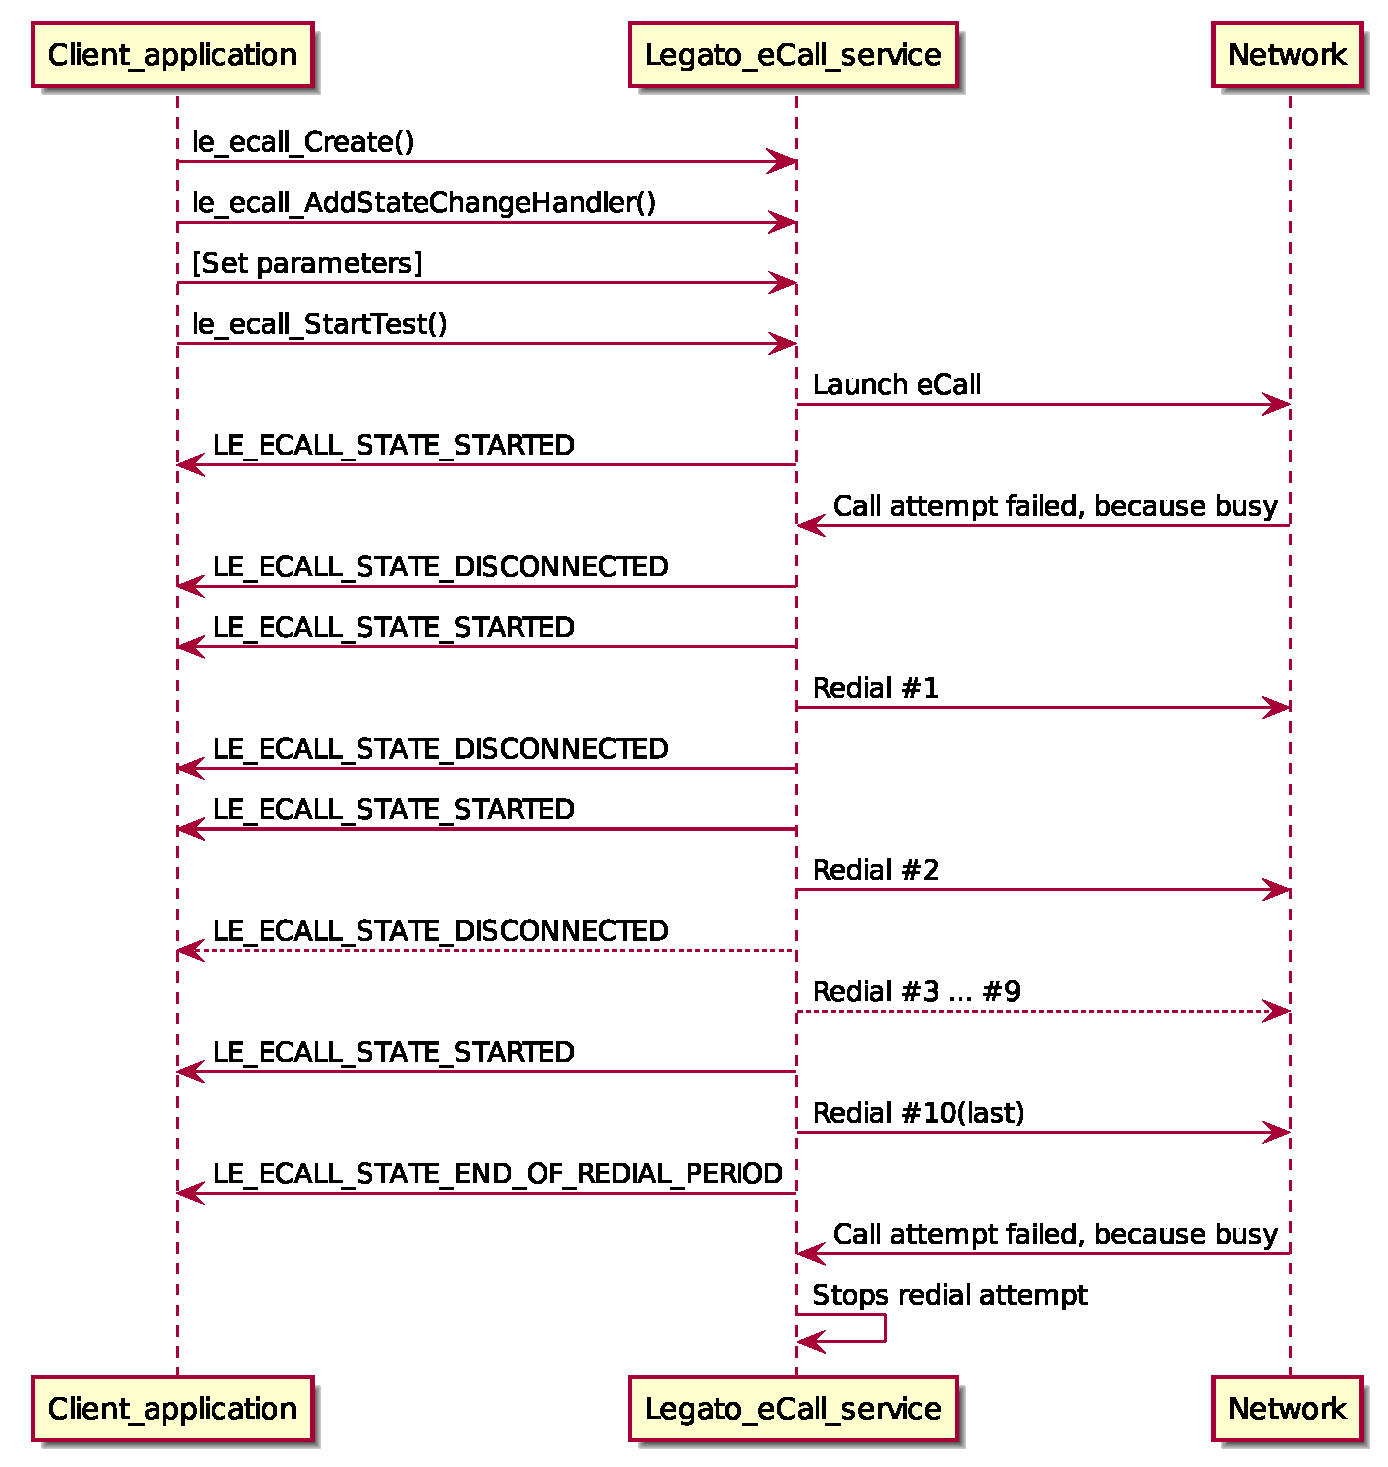
\includegraphics[width=\textwidth,height=\textheight/2,keepaspectratio=true]{EraGlonass_eCall_and_callFails}}
\end{DoxyImageNoCaption}


P\+AN EU redialing\+: The P\+AN European redialing has different restrictions. Before the call is connected the first time, there is no formal restriction to the number of retries. It is up to the app to implement the retry limit as there is no formal restriction.

\begin{DoxyNote}{Note}
If first connection is unsuccessful I\+VS redials until find the network coverage.
\end{DoxyNote}
If a call has been connected once before, and the M\+SD has not yet been sent, it has 120 seconds to reconnect the call. The 120 seconds are counted from the time the connected call was disconnected. This is because a P\+AN European e\+Call P\+S\+AP should call back after 3 minutes.

If the M\+SD has been successfully sent, there will be no redials from the I\+VS if the call is disconnected.

The retries are spaced out in time. The default is a 30 seconds interval between each start of each call attempt. It can be changed via \hyperlink{le__ecall__interface_8h_af90a8602d4b1d0cacaa3971c508dd188}{le\+\_\+ecall\+\_\+\+Set\+Interval\+Between\+Dial\+Attempts()}. If a call attempt takes longer than 30 seconds before failing, it will start directly after 1 second.

Following diagram shows redial mechanism for P\+A\+N-\/\+EU ecall if call fails\+:


\begin{DoxyImageNoCaption}
  \mbox{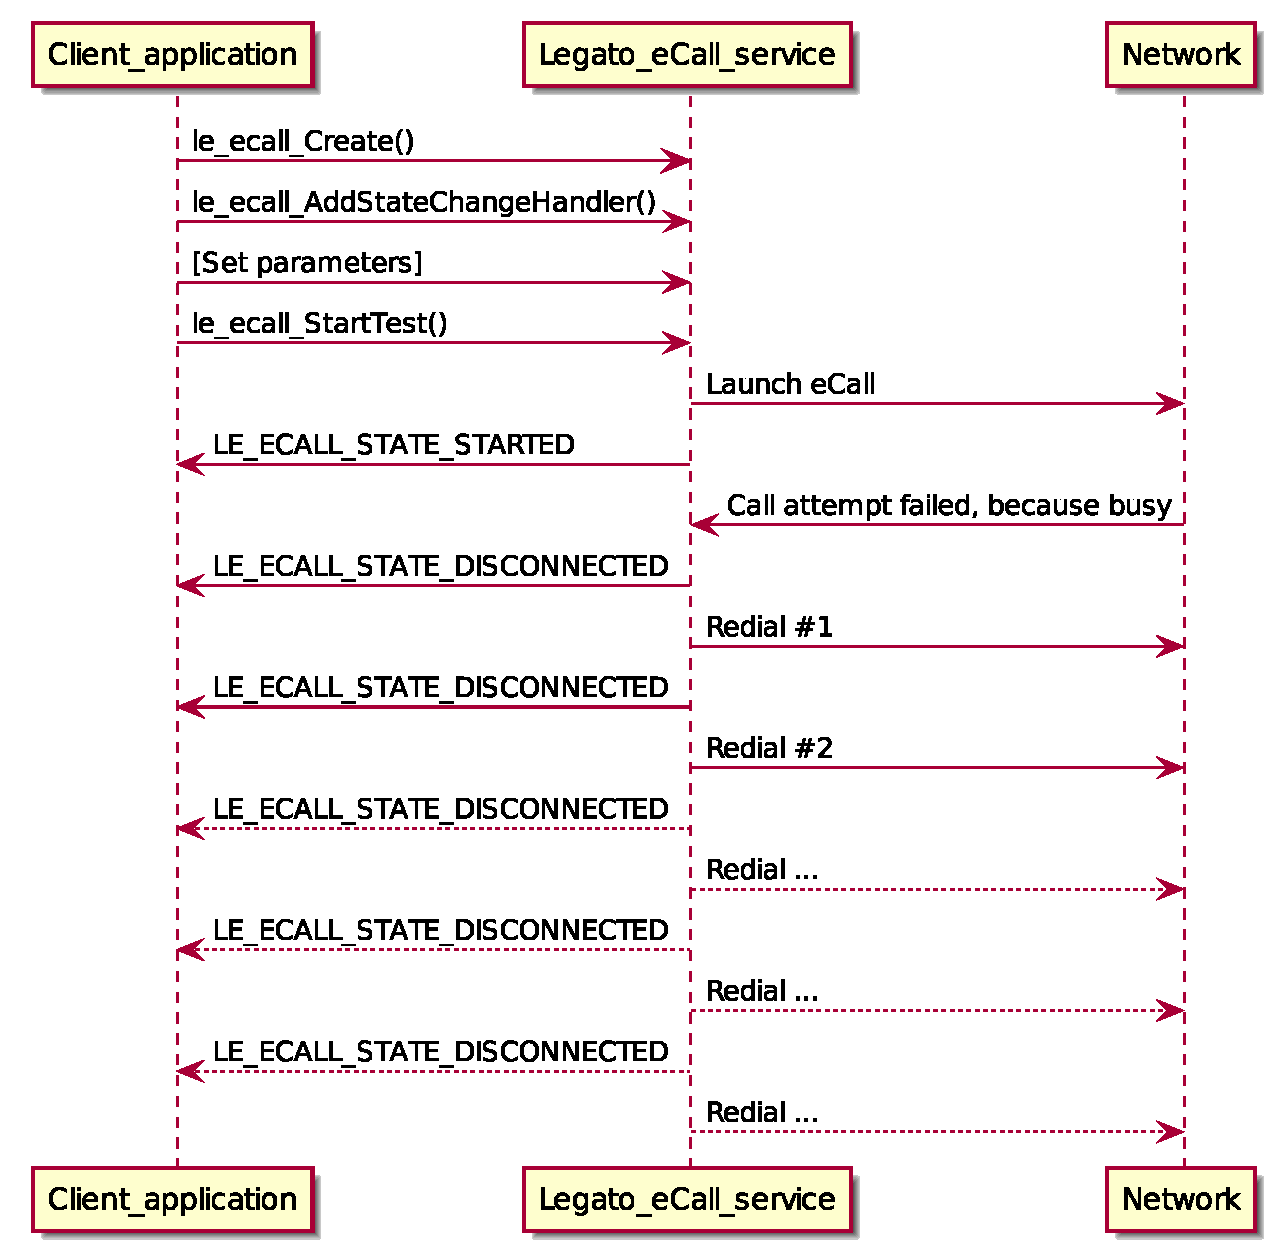
\includegraphics[width=\textwidth,height=\textheight/2,keepaspectratio=true]{PanEU_eCall_and_callFails}}
\end{DoxyImageNoCaption}


Following diagram shows redial mechanism for P\+A\+N-\/\+EU ecall if call connects and fails\+:


\begin{DoxyImageNoCaption}
  \mbox{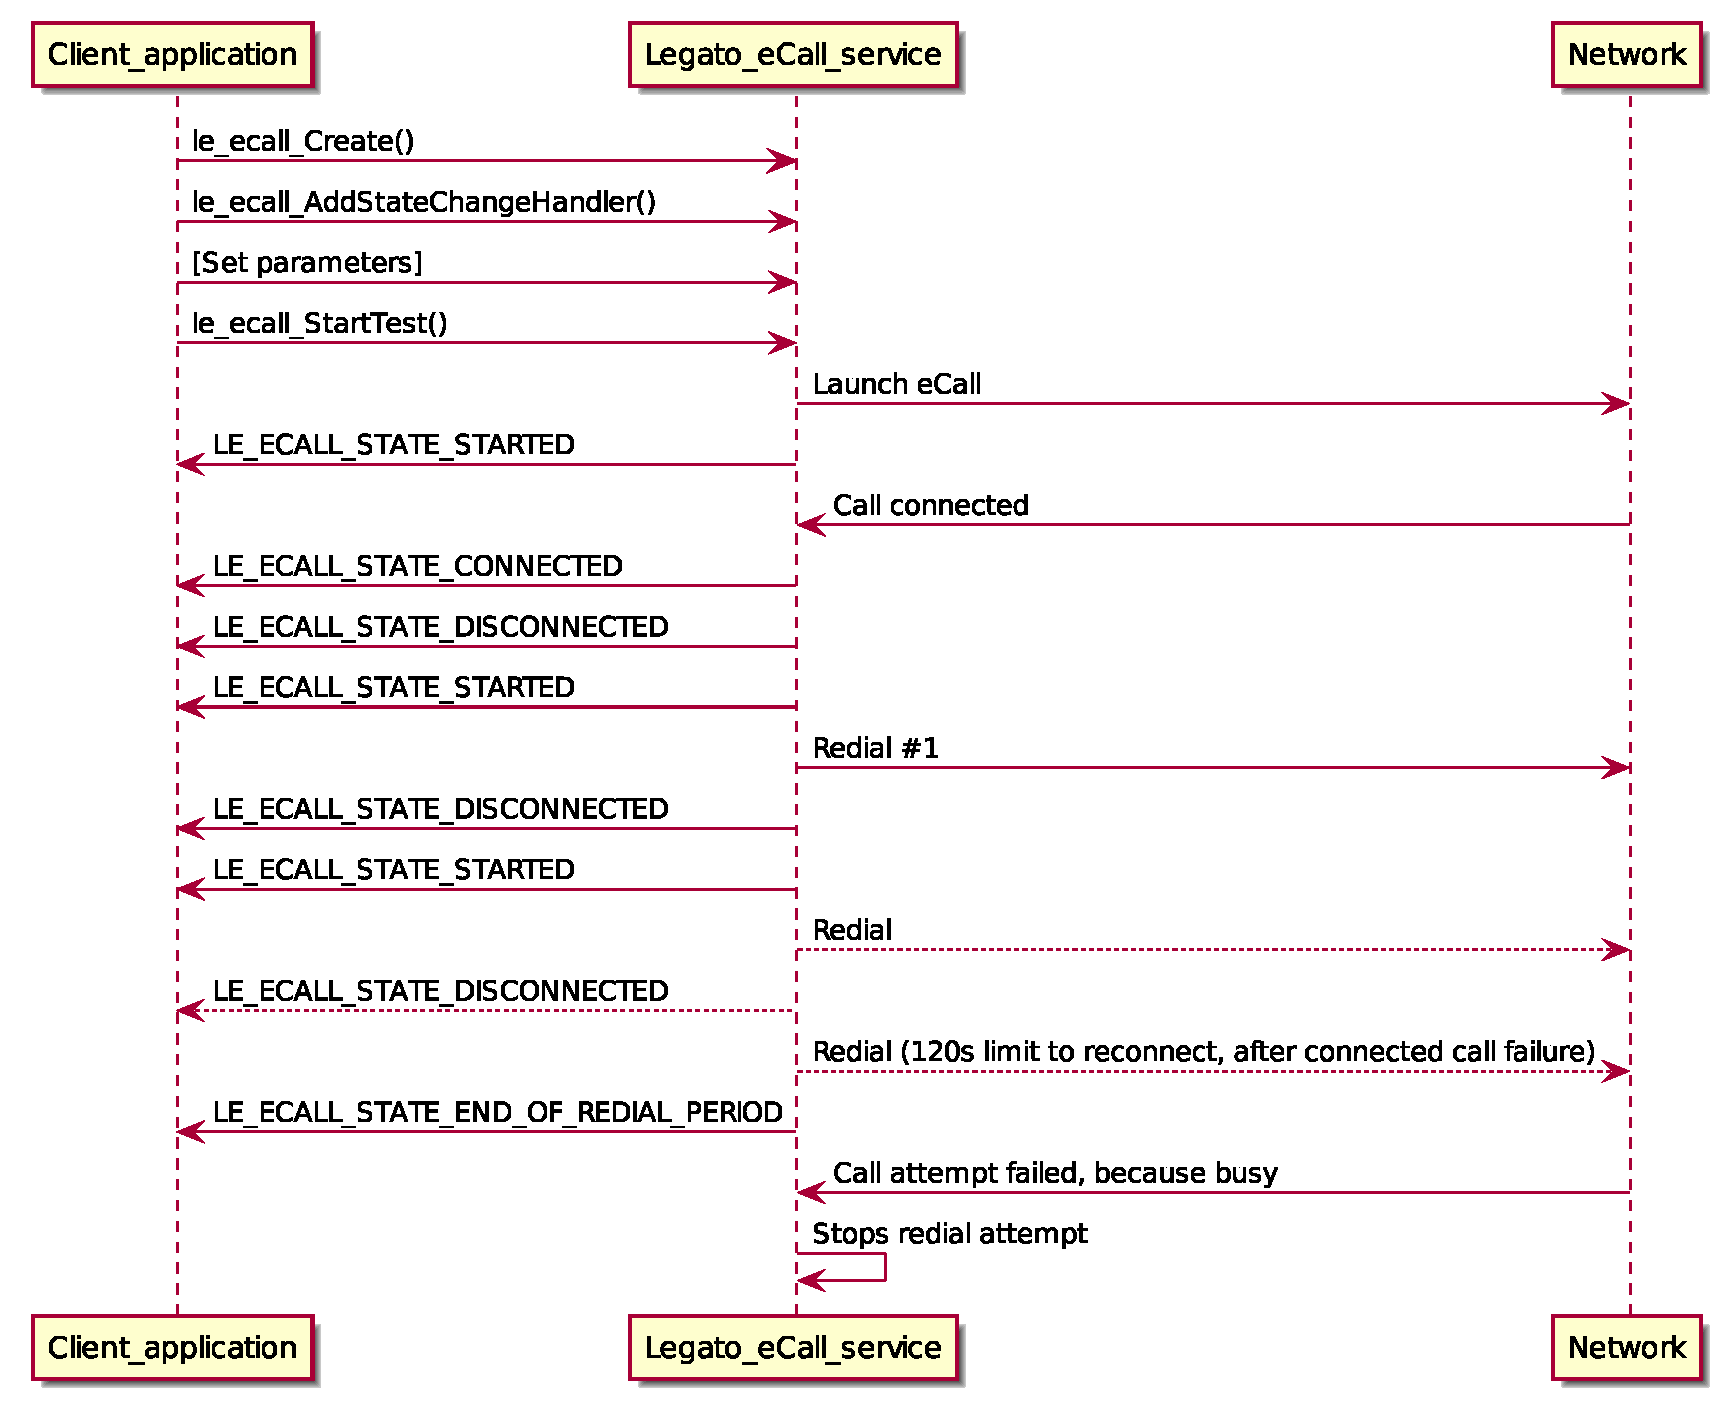
\includegraphics[width=\textwidth,height=\textheight/2,keepaspectratio=true]{PanEU_eCallConnects_thenFails}}
\end{DoxyImageNoCaption}
\hypertarget{c_SDD_eCall_le_ecall_configuration}{}\subsection{e\+Call configuration}\label{c_SDD_eCall_le_ecall_configuration}
Some parameters used by the e\+Call service can be configured through A\+P\+Is. This includes the number to dial, the deregistration time, the redial interval, and some M\+SD information.\hypertarget{c_SDD_eCall_le_ecall_configuration_callNumber}{}\subsubsection{e\+Call number}\label{c_SDD_eCall_le_ecall_configuration_callNumber}
By default, the number to dial is read from the F\+D\+N/\+S\+DN (Fixed Dialling Numbers/\+Service Dialling Numbers) of the U/\+S\+IM, depending upon the e\+Call operating mode.

However, the P\+S\+AP phone number can be queried and set with\+:
\begin{DoxyItemize}
\item \hyperlink{le__ecall__interface_8h_a959c53f03bb85f1071fcf7cb58e3067e}{le\+\_\+ecall\+\_\+\+Get\+Psap\+Number()}
\item \hyperlink{le__ecall__interface_8h_abf9c09914c55cdbe72df1433f60f6e51}{le\+\_\+ecall\+\_\+\+Set\+Psap\+Number()}
\end{DoxyItemize}

For e\+Call Test call, if U\+S\+IM is an e\+Call Only, the A\+PI \hyperlink{le__ecall__interface_8h_a034c442fd7c6650ed956822a561c0104}{le\+\_\+ecall\+\_\+\+Use\+U\+Sim\+Numbers()} shall be used in order to dials first index stored into F\+D\+N/\+S\+DN directory. It is possible to use \hyperlink{le__ecall__interface_8h_abf9c09914c55cdbe72df1433f60f6e51}{le\+\_\+ecall\+\_\+\+Set\+Psap\+Number()} if the P\+S\+AP number is the same as the number stored into first index of F\+DN directory. If U\+S\+IM is not e\+Call Only but\+\_\+le\+\_\+ecall\+\_\+\+Force\+Only\+Mode is forced to simulate e\+Call\+Only behavior the A\+PI \hyperlink{le__ecall__interface_8h_a034c442fd7c6650ed956822a561c0104}{le\+\_\+ecall\+\_\+\+Use\+U\+Sim\+Numbers()} may be used. In this case, the P\+S\+AP number should be stored into the first index of F\+DN directory and the facility lock on F\+DN should be activated. P\+S\+AP number shall be defined before to start e\+Call Test. It is not possible to set it when e\+Call session is on progress.


\begin{DoxyCodeInclude}
    \hyperlink{le__log_8h_a7cd2daa3d4af1de4d29e0eed95187484}{LE\_ASSERT\_OK}(\hyperlink{le__ecall__interface_8h_abf9c09914c55cdbe72df1433f60f6e51}{le\_ecall\_SetPsapNumber}(\textcolor{stringliteral}{"0102030405"}));

    \textcolor{keywordtype}{char} psapNumber[\hyperlink{le__mdm_defs__interface_8h_ae6d4a4c7892f14d1e340f8df083d479f}{LE\_MDMDEFS\_PHONE\_NUM\_MAX\_BYTES}] = \{0\};
    \hyperlink{le__log_8h_a7cd2daa3d4af1de4d29e0eed95187484}{LE\_ASSERT\_OK}(\hyperlink{le__ecall__interface_8h_a959c53f03bb85f1071fcf7cb58e3067e}{le\_ecall\_GetPsapNumber}(psapNumber, \textcolor{keyword}{sizeof}(psapNumber)));
    \hyperlink{le__log_8h_a23e6d206faa64f612045d688cdde5808}{LE\_INFO}(\textcolor{stringliteral}{"PSAP number: %s"}, psapNumber);
\end{DoxyCodeInclude}
 \begin{DoxyNote}{Note}
That P\+S\+AP number is not applied to a manual or an automatically initiated e\+Call. For these modes, an emergency call is launched.
\end{DoxyNote}
\begin{DoxyWarning}{Warning}
These two functions don\textquotesingle{}t modify or read the U/\+S\+IM content.
\end{DoxyWarning}
\hyperlink{le__ecall__interface_8h_a034c442fd7c6650ed956822a561c0104}{le\+\_\+ecall\+\_\+\+Use\+U\+Sim\+Numbers()} A\+PI can be called to request the modem to read the number to dial from the F\+D\+N/\+S\+DN of the U/\+S\+IM, depending upon the e\+Call operating mode.\hypertarget{c_SDD_eCall_le_ecall_configuration_nad}{}\subsubsection{N\+A\+D deregistration time}\label{c_SDD_eCall_le_ecall_configuration_nad}
The N\+AD (Network Access Device, i.\+e. the Modem) deregistration time value can be set with the \hyperlink{le__ecall__interface_8h_a66e454e84db7d337d76bc867b57891a1}{le\+\_\+ecall\+\_\+\+Set\+Nad\+Deregistration\+Time()} A\+PI and retrieved with the \hyperlink{le__ecall__interface_8h_a0f24b673049d51baf132ace25e2fa161}{le\+\_\+ecall\+\_\+\+Get\+Nad\+Deregistration\+Time()} A\+PI.


\begin{DoxyEnumerate}
\item P\+A\+N-\/\+E\+U\+R\+O\+P\+E\+AN standard ({\itshape EN 16062}) defines the T9 and T10 timers. After an e\+Call clear-\/down, an {\bfseries e\+Call only} I\+VS shall\+:
\begin{DoxyItemize}
\item Remain registered on the network for at least the duration of T9, which is set to one hour by default.
\item Deregister from the network after the expiration of T10, which duration is set to twelve hours by default.
\end{DoxyItemize}
\item E\+R\+A-\/\+G\+L\+O\+N\+A\+SS standard ({\itshape E\+N\+G\+\_\+\+G\+O\+S\+T\+\_\+\+R\+\_\+54620}) defines the N\+A\+D\+\_\+\+D\+E\+R\+E\+G\+I\+S\+T\+R\+A\+T\+I\+O\+N\+\_\+\+T\+I\+ME with a minimal value of two hours and a maximum value of twelve hours. After an e\+Call clear-\/down, the I\+VS shall remain registered on the network and deregister from the network after the expiration of the N\+A\+D\+\_\+\+D\+E\+R\+E\+G\+I\+S\+T\+R\+A\+T\+I\+O\+N\+\_\+\+T\+I\+ME.
\end{DoxyEnumerate}

The \hyperlink{le__ecall__interface_8h_a66e454e84db7d337d76bc867b57891a1}{le\+\_\+ecall\+\_\+\+Set\+Nad\+Deregistration\+Time()} A\+PI is used to set the duration of a {\itshape deregistration timer}\+: after an e\+Call clear-\/down, the I\+VS remains registered on the network for the duration of this timer and then automatically deregisters from the network upon its expiration.


\begin{DoxyCodeInclude}
    \hyperlink{le__log_8h_a7cd2daa3d4af1de4d29e0eed95187484}{LE\_ASSERT\_OK}(\hyperlink{le__ecall__interface_8h_a66e454e84db7d337d76bc867b57891a1}{le\_ecall\_SetNadDeregistrationTime}(180));

    uint16\_t deregistrationTime = 0;
    \hyperlink{le__log_8h_a7cd2daa3d4af1de4d29e0eed95187484}{LE\_ASSERT\_OK}(\hyperlink{le__ecall__interface_8h_a0f24b673049d51baf132ace25e2fa161}{le\_ecall\_GetNadDeregistrationTime}(&
      deregistrationTime));
    \hyperlink{le__log_8h_a23e6d206faa64f612045d688cdde5808}{LE\_INFO}(\textcolor{stringliteral}{"Deregistration time: %d minutes"}, deregistrationTime);
\end{DoxyCodeInclude}
 \hypertarget{c_SDD_eCall_le_ecall_configuration_nad_panEU}{}\paragraph{P\+A\+N-\/\+E\+U\+R\+O\+P\+E\+A\+N standard}\label{c_SDD_eCall_le_ecall_configuration_nad_panEU}
As the T9 timer duration is fixed to one hour, the notified events depend on the {\itshape deregistration timer} duration\+:
\begin{DoxyItemize}
\item If its duration is set to one hour, the \hyperlink{le__ecall__interface_8h_a233609e4724e549a1405f9177c0a07dda445e9365be6aac0b3403568d423ce6c5}{L\+E\+\_\+\+E\+C\+A\+L\+L\+\_\+\+S\+T\+A\+T\+E\+\_\+\+T\+I\+M\+E\+O\+U\+T\+\_\+\+T9} event will be reported. In this case deregistration is automatically performed when the T9 timeout indication is received.
\item If its duration is set to more than one hour and less than twelve hours then the \hyperlink{le__ecall__interface_8h_a233609e4724e549a1405f9177c0a07ddadafcb8d0490beb3d2778fadcbaeb8c11}{L\+E\+\_\+\+E\+C\+A\+L\+L\+\_\+\+S\+T\+A\+T\+E\+\_\+\+T\+I\+M\+E\+O\+U\+T\+\_\+\+T10} event will be reported when the {\itshape deregistration timer} expires. The T9 timeout (\hyperlink{le__ecall__interface_8h_a233609e4724e549a1405f9177c0a07dda445e9365be6aac0b3403568d423ce6c5}{L\+E\+\_\+\+E\+C\+A\+L\+L\+\_\+\+S\+T\+A\+T\+E\+\_\+\+T\+I\+M\+E\+O\+U\+T\+\_\+\+T9} event) will not be notified. In this case deregistration is automatically performed when the {\itshape deregistration timer} expires, provided that the application didn\textquotesingle{}t already deregister from the network before.
\end{DoxyItemize}\hypertarget{c_SDD_eCall_le_ecall_configuration_nad_eraGlonass}{}\paragraph{E\+R\+A-\/\+G\+L\+O\+N\+A\+S\+S standard}\label{c_SDD_eCall_le_ecall_configuration_nad_eraGlonass}

\begin{DoxyItemize}
\item The \hyperlink{le__ecall__interface_8h_a233609e4724e549a1405f9177c0a07dda445e9365be6aac0b3403568d423ce6c5}{L\+E\+\_\+\+E\+C\+A\+L\+L\+\_\+\+S\+T\+A\+T\+E\+\_\+\+T\+I\+M\+E\+O\+U\+T\+\_\+\+T9} event is not reported as it is not defined in the E\+R\+A-\/\+G\+L\+O\+N\+A\+SS standard.
\item The N\+A\+D\+\_\+\+D\+E\+R\+E\+G\+I\+S\+T\+R\+A\+T\+I\+O\+N\+\_\+\+T\+I\+ME default value is eight hours, as defined by {\itshape G\+O\+S\+T\+\_\+R 54620 Table A.\+1}. It can be changed with \hyperlink{le__ecall__interface_8h_a66e454e84db7d337d76bc867b57891a1}{le\+\_\+ecall\+\_\+\+Set\+Nad\+Deregistration\+Time()} and the value must be set between two and twelve hours.
\item The \hyperlink{le__ecall__interface_8h_a233609e4724e549a1405f9177c0a07ddadafcb8d0490beb3d2778fadcbaeb8c11}{L\+E\+\_\+\+E\+C\+A\+L\+L\+\_\+\+S\+T\+A\+T\+E\+\_\+\+T\+I\+M\+E\+O\+U\+T\+\_\+\+T10} event will be reported when the N\+A\+D\+\_\+\+D\+E\+R\+E\+G\+I\+S\+T\+R\+A\+T\+I\+O\+N\+\_\+\+T\+I\+ME expires. In this case deregistration is automatically performed when the timer expires.
\end{DoxyItemize}\hypertarget{c_SDD_eCall_le_ecall_configuration_nad_timerValue}{}\paragraph{Timer value}\label{c_SDD_eCall_le_ecall_configuration_nad_timerValue}
Although the time is set in minutes the value is taken in hours, for example\+:
\begin{DoxyItemize}
\item from 1 to 60 minutes -\/$>$ 1 hour
\item from 61 to 120 minutes -\/$>$ 2 hours, etc.
\end{DoxyItemize}

Example\+: if {\ttfamily dereg\+Time} parameter unit is minutes, the effective time is\+: 
\begin{DoxyCode}
ECallConfiguration.nad\_deregistration\_time = (deregTime+59)/60; 
\end{DoxyCode}


After termination of an emergency call the in-\/vehicle system remains registered on the network for the period of time, defined by the parameter N\+A\+D\+\_\+\+D\+E\+R\+E\+G\+I\+S\+T\+R\+A\+T\+I\+O\+N\+\_\+\+T\+I\+ME.

\begin{DoxyWarning}{Warning}
Be sure to check the possible values of N\+A\+D\+\_\+\+D\+E\+R\+E\+G\+I\+S\+T\+R\+A\+T\+I\+O\+N\+\_\+\+T\+I\+ME for your specific platform.
\end{DoxyWarning}
\hypertarget{c_SDD_eCall_le_ecall_configuration_redialInterval}{}\subsubsection{Redial interval}\label{c_SDD_eCall_le_ecall_configuration_redialInterval}
The minimum interval time value between dial attempts can be set or get with\+:
\begin{DoxyItemize}
\item \hyperlink{le__ecall__interface_8h_af90a8602d4b1d0cacaa3971c508dd188}{le\+\_\+ecall\+\_\+\+Set\+Interval\+Between\+Dial\+Attempts()}
\item \hyperlink{le__ecall__interface_8h_a3a24ae5a007d0c43db2bc55caa43c19d}{le\+\_\+ecall\+\_\+\+Get\+Interval\+Between\+Dial\+Attempts()}
\end{DoxyItemize}


\begin{DoxyCodeInclude}
    \hyperlink{le__log_8h_a7cd2daa3d4af1de4d29e0eed95187484}{LE\_ASSERT\_OK}(\hyperlink{le__ecall__interface_8h_af90a8602d4b1d0cacaa3971c508dd188}{le\_ecall\_SetIntervalBetweenDialAttempts}
      (30));

    uint16\_t pause = 0;
    \hyperlink{le__log_8h_a7cd2daa3d4af1de4d29e0eed95187484}{LE\_ASSERT\_OK}(\hyperlink{le__ecall__interface_8h_a3a24ae5a007d0c43db2bc55caa43c19d}{le\_ecall\_GetIntervalBetweenDialAttempts}
      (&pause));
    \hyperlink{le__log_8h_a23e6d206faa64f612045d688cdde5808}{LE\_INFO}(\textcolor{stringliteral}{"Interval between dial attempts: %d seconds"}, pause);
\end{DoxyCodeInclude}
 The default value is set to 30 seconds.

The time is counted from the start of the first dial attempt.

If a call attempt takes longer than the Interval\+Between\+Dial\+Attempts before failing, it will start directly after 1 second. When the redial is initiated because of a call drop then it pauses only 1 second to allow the network stack to get ready before starting a new dial attempt.

If less time than the Interval\+Between\+Dial\+Attempts has expired during the dial attempt, it will wait for time the Interval\+Between\+Dial\+Attempts seconds to allow hangup before redialing.

\hyperlink{le__ecall__interface_8h_af90a8602d4b1d0cacaa3971c508dd188}{le\+\_\+ecall\+\_\+\+Set\+Interval\+Between\+Dial\+Attempts()} is available for both manual and test modes.\hypertarget{c_SDD_eCall_le_ecall_configuration_misc}{}\subsubsection{Miscellaneous}\label{c_SDD_eCall_le_ecall_configuration_misc}
The preferred system standard defaults to P\+A\+N-\/\+E\+U\+R\+O\+P\+E\+AN It can be set an gotten with the following functions\+:
\begin{DoxyItemize}
\item \hyperlink{le__ecall__interface_8h_a1b492b42490b319fcc228e52f8694307}{le\+\_\+ecall\+\_\+\+Set\+System\+Standard()}
\item \hyperlink{le__ecall__interface_8h_abfb468cf1e977e9b2444d13617322331}{le\+\_\+ecall\+\_\+\+Get\+System\+Standard()}
\end{DoxyItemize}


\begin{DoxyCodeInclude}
    \hyperlink{le__log_8h_a7cd2daa3d4af1de4d29e0eed95187484}{LE\_ASSERT\_OK}(\hyperlink{le__ecall__interface_8h_a1b492b42490b319fcc228e52f8694307}{le\_ecall\_SetSystemStandard}(
      \hyperlink{le__ecall__interface_8h_a38a79a5123761b6808ea58b4f343579baddc50d7d4524fffc7388c5753ce5a299}{LE\_ECALL\_ERA\_GLONASS}));

    \hyperlink{le__ecall__interface_8h_a38a79a5123761b6808ea58b4f343579b}{le\_ecall\_SystemStandard\_t} systemStandard;
    \hyperlink{le__log_8h_a7cd2daa3d4af1de4d29e0eed95187484}{LE\_ASSERT\_OK}(\hyperlink{le__ecall__interface_8h_abfb468cf1e977e9b2444d13617322331}{le\_ecall\_GetSystemStandard}(&systemStandard));
    \hyperlink{le__log_8h_a23e6d206faa64f612045d688cdde5808}{LE\_INFO}(\textcolor{stringliteral}{"System standard: %d"}, systemStandard);
\end{DoxyCodeInclude}
 The M\+SD version can be set and and gotten with the following functions\+:
\begin{DoxyItemize}
\item \hyperlink{le__ecall__interface_8h_a4d698cd7bde3b33e191453d31bc7c9d1}{le\+\_\+ecall\+\_\+\+Set\+Msd\+Version()}
\item \hyperlink{le__ecall__interface_8h_a4875975bc3f3c8fb78b43ae40322eedd}{le\+\_\+ecall\+\_\+\+Get\+Msd\+Version()}
\end{DoxyItemize}


\begin{DoxyCodeInclude}
    \hyperlink{le__log_8h_a7cd2daa3d4af1de4d29e0eed95187484}{LE\_ASSERT\_OK}(\hyperlink{le__ecall__interface_8h_a4d698cd7bde3b33e191453d31bc7c9d1}{le\_ecall\_SetMsdVersion}(1))

    uint32\_t msdVersion = 0;
    \hyperlink{le__log_8h_a7cd2daa3d4af1de4d29e0eed95187484}{LE\_ASSERT\_OK}(\hyperlink{le__ecall__interface_8h_a4875975bc3f3c8fb78b43ae40322eedd}{le\_ecall\_GetMsdVersion}(&msdVersion));
    \hyperlink{le__log_8h_a23e6d206faa64f612045d688cdde5808}{LE\_INFO}("MSD version: %d", msdVersion);
\end{DoxyCodeInclude}
 The vehicle type can be set and gotten with the following functions\+:
\begin{DoxyItemize}
\item \hyperlink{le__ecall__interface_8h_a291bd0a938266981a8cb6eb836c45b37}{le\+\_\+ecall\+\_\+\+Set\+Vehicle\+Type()}
\item \hyperlink{le__ecall__interface_8h_ab7cdf7de011b9c8edaec790b360dded6}{le\+\_\+ecall\+\_\+\+Get\+Vehicle\+Type()}
\end{DoxyItemize}


\begin{DoxyCodeInclude}
    \hyperlink{le__log_8h_a7cd2daa3d4af1de4d29e0eed95187484}{LE\_ASSERT\_OK}(\hyperlink{le__ecall__interface_8h_a291bd0a938266981a8cb6eb836c45b37}{le\_ecall\_SetVehicleType}(
      \hyperlink{le__ecall__interface_8h_a90c7868842c599a89be72a1ff8609f09acf7dde2942af72d9656c0b753aab4880}{LE\_ECALL\_MSD\_VEHICLE\_BUS\_M2}));

    \hyperlink{le__ecall__interface_8h_a90c7868842c599a89be72a1ff8609f09}{le\_ecall\_MsdVehicleType\_t} vehicleType;
    \hyperlink{le__log_8h_a7cd2daa3d4af1de4d29e0eed95187484}{LE\_ASSERT\_OK}(\hyperlink{le__ecall__interface_8h_ab7cdf7de011b9c8edaec790b360dded6}{le\_ecall\_GetVehicleType}(&vehicleType));
    \hyperlink{le__log_8h_a23e6d206faa64f612045d688cdde5808}{LE\_INFO}(\textcolor{stringliteral}{"Vehicle type: %d"}, vehicleType);
\end{DoxyCodeInclude}
 The vehicle identifier can be set and gotten with the following functions\+:
\begin{DoxyItemize}
\item \hyperlink{le__ecall__interface_8h_aca95cc7f1d44d3acef601ea97714f748}{le\+\_\+ecall\+\_\+\+Set\+V\+I\+N()}
\item \hyperlink{le__ecall__interface_8h_acc26551a121b769ca0b358a8b6c47694}{le\+\_\+ecall\+\_\+\+Get\+V\+I\+N()}
\end{DoxyItemize}


\begin{DoxyCodeInclude}
    \hyperlink{le__log_8h_a7cd2daa3d4af1de4d29e0eed95187484}{LE\_ASSERT\_OK}(\hyperlink{le__ecall__interface_8h_aca95cc7f1d44d3acef601ea97714f748}{le\_ecall\_SetVIN}(\textcolor{stringliteral}{"VF37BRFVE12345678"}));

    \textcolor{keywordtype}{char} vin[\hyperlink{le__ecall__interface_8h_a0fce568162ff0d320cdea60adf4c9d3a}{LE\_ECALL\_VIN\_MAX\_BYTES}] = \{0\};
    \hyperlink{le__log_8h_a7cd2daa3d4af1de4d29e0eed95187484}{LE\_ASSERT\_OK}(\hyperlink{le__ecall__interface_8h_acc26551a121b769ca0b358a8b6c47694}{le\_ecall\_GetVIN}(vin, \textcolor{keyword}{sizeof}(vin)));
    \hyperlink{le__log_8h_a23e6d206faa64f612045d688cdde5808}{LE\_INFO}(\textcolor{stringliteral}{"VIN: %s"}, vin);
\end{DoxyCodeInclude}
 The propulsion type can be set and gotten with the following functions\+:
\begin{DoxyItemize}
\item \hyperlink{le__ecall__interface_8h_abb9c569b53f8c35b878c7c9ca159e1df}{le\+\_\+ecall\+\_\+\+Set\+Propulsion\+Type()}
\item \hyperlink{le__ecall__interface_8h_aea86cec8465c43f4cc71ac3c7879965a}{le\+\_\+ecall\+\_\+\+Get\+Propulsion\+Type()}
\end{DoxyItemize}


\begin{DoxyCodeInclude}
    \hyperlink{le__log_8h_a7cd2daa3d4af1de4d29e0eed95187484}{LE\_ASSERT\_OK}(\hyperlink{le__ecall__interface_8h_abb9c569b53f8c35b878c7c9ca159e1df}{le\_ecall\_SetPropulsionType}(
      \hyperlink{le__ecall__interface_8h_a10f3332edf213de92962a861b0fb6a1fa1f6166e6aec7ef156bc0a2d1b608ecf9}{LE\_ECALL\_PROPULSION\_TYPE\_OTHER}));

    \hyperlink{le__ecall__interface_8h_a10f3332edf213de92962a861b0fb6a1f}{le\_ecall\_PropulsionTypeBitMask\_t} propulsionType;
    \hyperlink{le__log_8h_a7cd2daa3d4af1de4d29e0eed95187484}{LE\_ASSERT\_OK}(\hyperlink{le__ecall__interface_8h_aea86cec8465c43f4cc71ac3c7879965a}{le\_ecall\_GetPropulsionType}(&propulsionType));
    \hyperlink{le__log_8h_a23e6d206faa64f612045d688cdde5808}{LE\_INFO}(\textcolor{stringliteral}{"Propulsion type: 0x%02x"}, propulsionType);
\end{DoxyCodeInclude}
 Copyright (C) Sierra Wireless Inc. 